% Copyright 2004 by Till Tantau <tantau@users.sourceforge.net>.
%
% In principle, this file can be redistributed and/or modified under
% the terms of the GNU Public License, version 2.
%
% However, this file is supposed to be a template to be modified
% for your own needs. For this reason, if you use this file as a
% template and not specifically distribute it as part of a another
% package/program, I grant the extra permission to freely copy and
% modify this file as you see fit and even to delete this copyright
% notice. 
% Adapted by Len Goff, 2019

\documentclass[8pt]{beamer}

% There are many different themes available for Beamer. A comprehensive
% list with examples is given here:

% http://deic.uab.es/~iblanes/beamer_gallery/index_by_theme.html
% You can uncomment the themes below if you would like to use a different
% one:
%\usetheme{AnnArbor}
%\usetheme{Antibes}
%\usetheme{Bergen}
%\usetheme{Berkeley}
%\usetheme{Berlin}
%\usetheme{Boadilla}
%\usetheme{boxes}
%\usetheme{CambridgeUS}
%\usetheme{Copenhagen}
%\usetheme{Darmstadt}
%\usetheme{default}
%\usetheme{Frankfurt}
%\usetheme{Goettingen}
%\usetheme{Hannover}
%\usetheme{Ilmenau}
%\usetheme{JuanLesPins}
%\usetheme{Luebeck}
\usetheme{Madrid}
%\usetheme{Malmoe}
%\usetheme{Marburg}
%\usetheme{Montpellier}
%\usetheme{PaloAlto}
%\usetheme{Pittsburgh}
%\usetheme{Rochester}
%\usetheme{Singapore}
%\usetheme{Szeged}
%\usetheme{Warsaw}
\usefonttheme{professionalfonts}
\usepackage{tikz,tikz-cd}
%Some code to format a hyperlink button
\setbeamertemplate{button}{\tikz[baseline={(0,-3.5pt)}]
	\node[
	inner xsep=5pt,
	inner ysep=1pt,
	draw=structure!80,
	fill=structure!50,
	rounded corners=4pt]  {\topskip0pt \normalsize\insertbuttontext};}
\newcommand{\lrp}[1]{\left(#1\right)}
\newcommand{\lrb}[1]{\left[#1\right]}
\newcommand{\lrc}[1]{\left\{#1\right\}}
\newcommand{\lrl}[1]{\langle#1\rangle}
\renewcommand{\exp}[1]{\textrm{exp}\lrc{#1}}
\renewcommand{\log}[1]{\textrm{log}\lrp{#1}}
\newcommand{\ch}{\chi^2}
\renewcommand{\d}{\text{d}}
\renewcommand{\ln}{\text{ln}}
\renewcommand{\b}[1]{\beta_{#1}}
\newcommand{\absl}[1]{\left|#1\right|}
\newcommand{\Prob}[1]{\textrm{Pr}\lrp{#1}}
\newcommand{\ml}[1]{\mathcal{#1}}
\newcommand{\m}{m_{h_k}}
\renewcommand{\c}{c_{h_k}}
\renewcommand{\lim}{\stackbin[n\to\infty]{}{\text{lim}}}
\renewcommand{\thefootnote}{\fnsymbol{footnote}}
\newcommand{\xa}{{{  x}_a^{\star}}}
\newcommand{\xt}{{{  x}_t^{\star}}}
\newcommand{\one}{\textit{1}}
\newcommand{\PO}{\mathcal{PO}}
\newcommand{\BF}{\mathcal{BF}}
\renewcommand{\tt}[1]{|| #1 X_{T/i}\beta_{T/i}||^2}
\newcommand{\bfCref}[1]{ \textbf{\Cref{#1}}}
\renewcommand{\sin}[1]{\textrm{sin}\lrp{#1}}
\newcommand{\hc}{\tilde{\beta}_{S^C_0}}
\newcommand{\hs}{\tilde{\beta}_{S_0}}
\newcommand{\ts}{\beta^0_{S_0}}
\newcommand{\F}{|F|}
\newcommand{\M}[1]{\mathcal{M}_{#1}}
\newcommand{\A}{|A|}
\newcommand{\T}{|T|}
\newcommand{\quy}[1]{\frac{y'#1y}{\sigma^2}}
\newcommand{\ff}[1]{\frac{#1}{2}}
\usepackage[utf8]{inputenc}
\usepackage{booktabs}
%Some packages that will be useful
\usepackage{pgfplots}
\usepackage{cancel}
\usepackage{caption}
\usepackage{array}
\usepackage{dcolumn}
\usepackage{mathtools}
\captionsetup{belowskip=-15pt,aboveskip=0pt}
\usepackage{stackrel}
\usepackage{subfigure}

\usepackage{sansmathaccent}
\pdfmapfile{+sansmathaccent.map}
\usepackage[]{algorithm2e}
\makeatletter
\g@addto@macro\normalsize{
\setlength\abovedisplayskip{4pt}
\setlength\belowdisplayskip{4pt}
\setlength\abovedisplayshortskip{4pt}
\setlength\belowdisplayshortskip{4pt}
}
\makeatother
\makeatletter
\renewcommand{\@algocf@capt@plain}{bottom}% formerly {bottom}
\makeatother
\usenavigationsymbolstemplate{}

\usepackage{array}
\newcolumntype{H}{>{\setbox0=\hbox\bgroup}c<{\egroup}@{}}
\usepackage{makecell}

\makeatletter
\def\thmhead@plain#1#2#3{%
	\thm@notefont{}% same as heading font
	\thmname{#1}\thmnumber{\@ifnotempty{#1}{ }\@upn{#2}}%
	\thmnote{ {\the\thm@notefont#3}}}
\let\thmhead\thmhead@plain
\itshape % body font
\makeatother

%Define normal density function for use in tikzpicture
\pgfmathdeclarefunction{gauss}{2}{%
	\pgfmathparse{3/(#2*sqrt(2*pi))*exp(-((x-#1)^2)/(2*#2^2))}%
}


%This allows adjustable spacing in itemize environment
\newenvironment{wideitemize}{\itemize\addtolength{\itemsep}{10pt}}{\enditemize}

%This allows slide numberering to not includethe title slide
\addtocounter{framenumber}{-1}
\addtobeamertemplate{navigation symbols}{}{%
	\usebeamerfont{footline}%
	\usebeamercolor[fg]{footline}%
	\hspace{1em}%
	%uncomment the below if you want frame numbers inside slide rather than in footline
	%\insertframenumber/\inserttotalframenumber
}

%
\newcommand{\backupbegin}{
	\newcounter{finalframe}
	\setcounter{finalframe}{\value{framenumber}}
}
\newcommand{\backupend}{
	\setcounter{framenumber}{\value{finalframe}}
}

\usetikzlibrary{decorations.pathreplacing,angles,quotes}
\usetikzlibrary{patterns}
\usetikzlibrary{positioning}
\usetikzlibrary{decorations.text}
\usetikzlibrary{decorations.pathmorphing}

%\title{Entangled instrumental variables}
\title[UNL (05/09/2022)]{CARMA: Novel Bayesian model for fine-mapping in meta-analysis studies}

% A subtitle is optional and this may be deleted

\author{Zikun Yang, Ph.D }

% (optional, but mostly needed)
\institute[CU]
{
	\small  Department of Biostatistics, Columbia University
}

	

\date{}

\usepackage{graphicx}
\usepackage{bbm}

\graphicspath{ {images/} }
\setbeamercovered{}

\begin{document}
%%%%%%%%%%%%%%%%%%%%%%%%%%%%%%%%%%%%%%%%%%%%%%%%%%%%%%%%%%%%%%%%%%%%%%%%%%%%%%%%%%%%%%
%%%%%%%%%%%%%%%%%%%%%%%%%%%%%%%%%%%%%%%%%%%%%%%%%%%%%%%%%%%%%%%%%%%%%%%%%%%%%%%%%%%%%%
\begin{frame}
  \titlepage
\end{frame}
\frame[t]{
\frametitle{Self introduction}
\begin{itemize}
\item Graduated from the Department of Statistics in Indiana University (Hoosiers!).
\item Thesis advisor: Andrew Womack, Ph.D.
\item Doctor thesis: Model selection in high-dimensional regime with Bayesian statistics.
\item Currently working in the Department of Biostatistics in Columbia University
\item PI: Iuliana Ionita-Laza, Ph.D.
\item Researches: statistical genetics with applications on genomic data, e.g. GWAS, MPRA etc.. 
\end{itemize}
\begin{columns}
\begin{column}[b]{0.45\textwidth}
\begin{block}{Bayesian statistics}
\begin{itemize}
\item Proposed a new Bayesian shrinkage prior, Heavy-tailed Horseshoe prior. Comparing to HS, HS+, D-L priors, showed better MSE, better KL risk bounds, better posterior concentration, also the asymptotically minimax risk rate in $L_2$ norm.
\item Showed posterior model selection consistency under the scenario of growing true model with Zellner-Siow and Poisson prior. 
\end{itemize}
\end{block}
\end{column}%
\hfill%
\begin{column}[b]{0.45\textwidth}
\begin{block}{Bayesian statistical genetics}
\begin{itemize}
\item Proposed CARMA fine-mapping method. 
\item Proposed PO-EN model, which is tailored to the data structure of the massively parallel reporter assays (MPRAs). Using positive and unlabeled/background data together with  epigenetic features to build presence-only prediction models of regulatory effects of variants.
\end{itemize}
\end{block}
\end{column}%
\end{columns}
}
%%%%%%%%%%%%%%%%%%%%%%%%%%%%%%%%%%%%%
\frame{
\frametitle{Content of today's talk }
\large
\begin{block}{Content}
\begin{itemize}
\item Briefly review the background story of genetics research (GWAS)
\item Motivate for the fine-mapping methods
\item Challenges of the new method and how we address the challenges
\item Simulation and real-data analysis
\item {\bf Remark:} More focusing on the features and challenges of genetic data instead of statistical properties or details of the newly proposed model.  
\end{itemize}
\end{block}

}
%%%%%%%%%%%%%%%%%%%%%%%%%%%%%%%%%%%%%
\frame[t]{
\frametitle{Genome-wide association studies (GWAS)}
\begin{block}{From genome-wide associations to candidate causal variants  }
\begin{itemize}
\item Common complex human traits, quantitative traits (BMI) or diseases (T2D), often result from multiple environmental and genetic causes.
\item GWAS have been widely used to identify the genomic regions on chromosomes that harbour genetic determinants of complex traits.
\item Many putative loci (genomic regions) of genetic disease has discovered based on GWAS
\item The natural next step is to identify putative causal genetic variants, i.e. single-nucleotide polymorphisms (SNPs), at these loci.
\end{itemize}
\end{block}
}

%%%%%%%%%%%%%%%%%%%%%%%%%%%%%%%%%%%%%
\frame[t]{ %1
\frametitle{GWAS pipeline}
\fontsize{7pt}{7pt}
\begin{columns}[T] % align columns
\begin{column}{.56\textwidth}
\begin{figure}[htbp] %  figure placement: here, top, bottom, or page
   \centering
   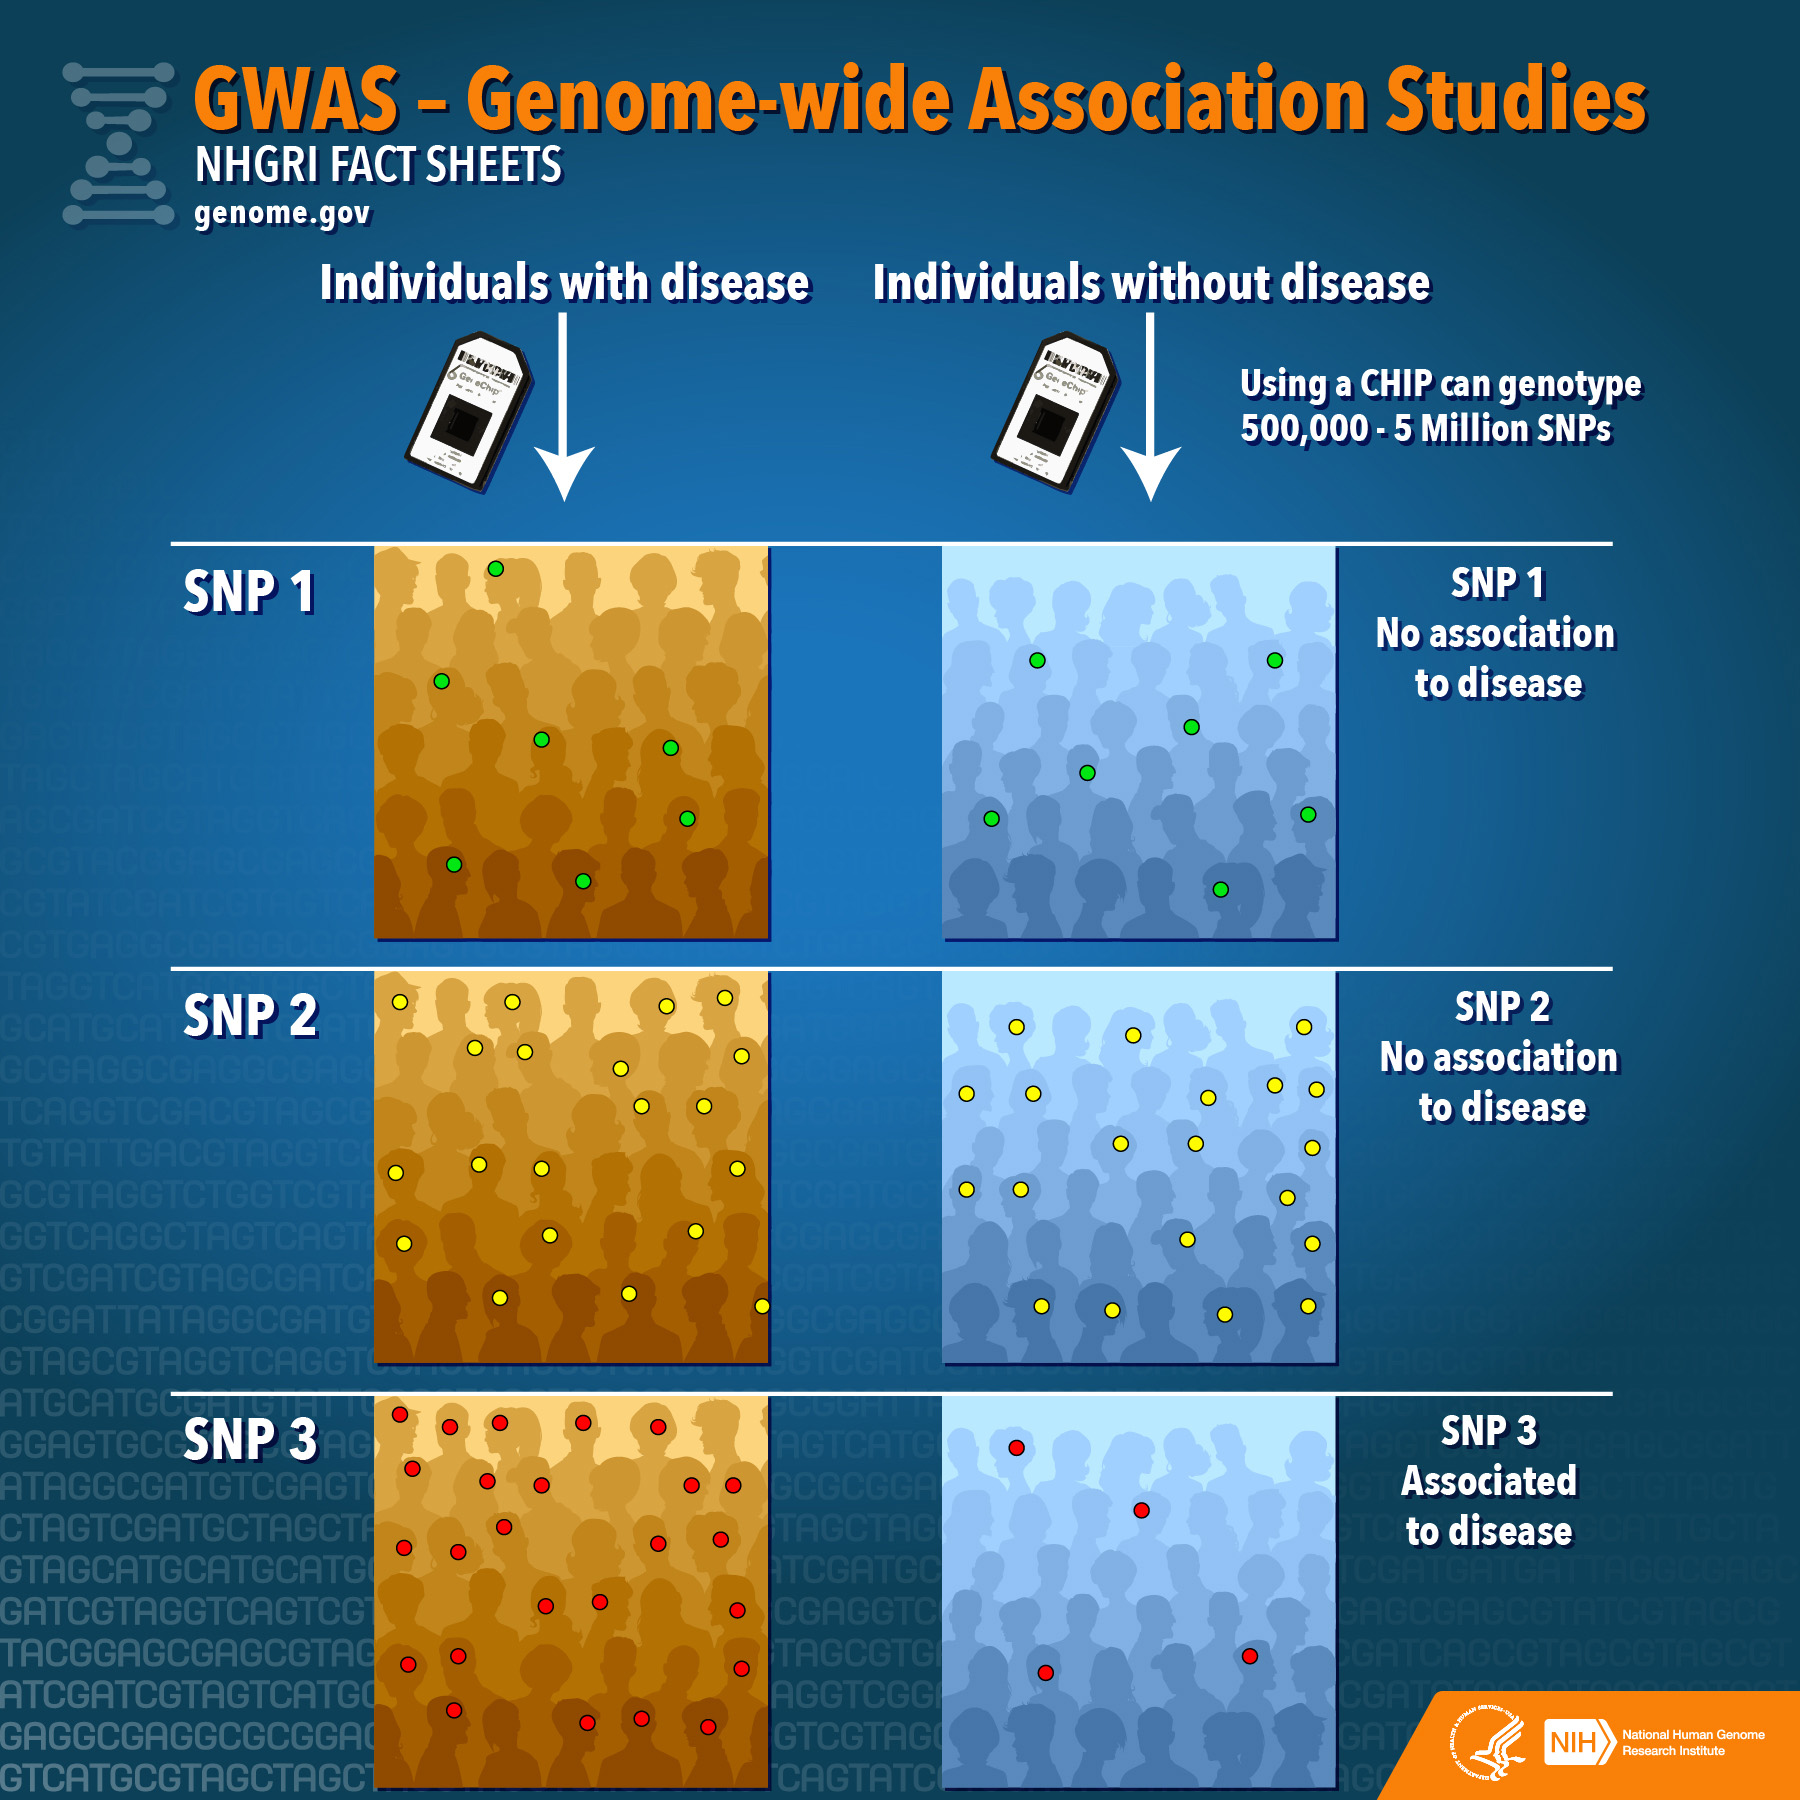
\includegraphics[width=2in]{./plots/GWAS_1.jpeg} 
   \\
   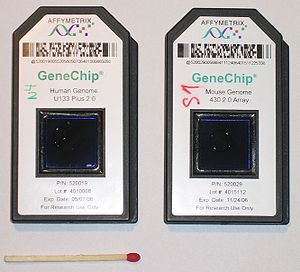
\includegraphics[width=1in]{./plots/gwas_chip.jpeg} 
   \caption{GWAS study and chips. }
   \label{fig:example}
\end{figure}
\end{column}%
\hfill%
\begin{column}{.40\textwidth}
\begin{block}{\small GWAS}
\begin{itemize}
\item Recruit subjects.
\item Collect trait (binary or quantitative) 
\item Collect covariates of subjects, e.g. age, gender etc.
\item Collect genotypes (imputed) through genotyping techniques (chips)
\end{itemize}
\end{block}
\pause
\begin{block}{\small Marginal association of SNPs}
\begin{itemize}
\item Run linear mixed models or generalized mixed models 
\item The result of LMM is the marginal association of testing SNP to the complex trait. 
\end{itemize}
\end{block}
\end{column}%
\end{columns}
}

%%%%%%%%%%%%%%%%%%%%%%%%%%%%%%%%%%%%%
%%%%%%%%%%%%%%%%%%%%%%%%%%%%%%%%%%%%%
\frame[t]{%2
\frametitle{GWAS pipeline}
\fontsize{7pt}{7pt}
\begin{columns}[T] % align columns
\begin{column}{.66\textwidth}
\begin{figure}[htbp] %  figure placement: here, top, bottom, or page
   \centering
   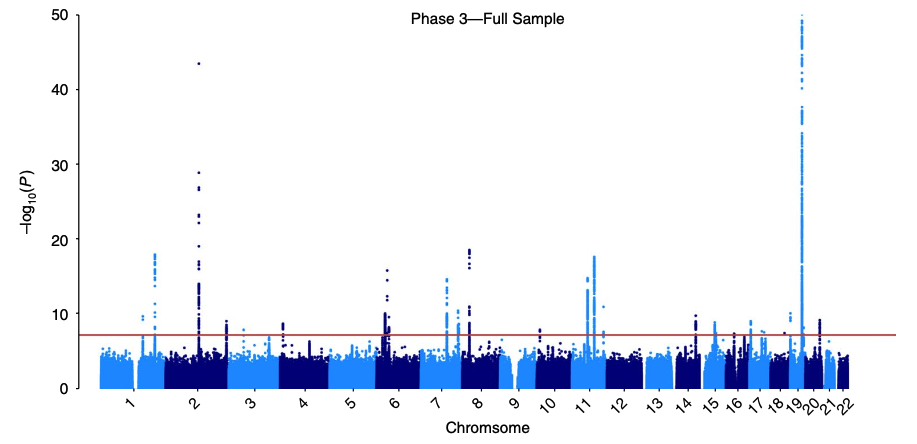
\includegraphics[width=3in]{./plots/manhattan.png} 
   \caption{Manhattan figure of Alzheimer's disease study\cite{jansen2019genome}. The y axis is $-\text{log}_{10}(\text{P-values})$, and the commonly-used genome-wide statistical significance threshold of P value is $< 5 \times 10^{-8}$ for a reliable GWAS results. }
   \label{fig:example}
\end{figure}
\end{column}%
\hfill%
\begin{column}{.30\textwidth}
\fontsize{7pt}{7pt}
\begin{block}{\small GWAS}
\begin{itemize}
\item Collect trait and genotypes (imputed)
\end{itemize}
\end{block}
\begin{block}{\small Marginal association of SNPs}
\begin{itemize}
\item Run linear mixed models or generalized mixed models 
\item Summarize results in Manhattan plot
\end{itemize}
\end{block}
\pause
\begin{block}{\small Investigate on independent genomic region (locus)}
\begin{itemize}
\item List of associated SNPs
\item Explore each independent regions
\end{itemize}
\end{block}
\end{column}%
\end{columns}
}

%%%%%%%%%%%%%%%%%%%%%%%%%%%%%%%%%%%%%
%%%%%%%%%%%%%%%%%%%%%%%%%%%%%%%%%%%%%
%%%%%%%%%%%%%%%%%%%%%%%%%%%%%%%%%%%%%
\frame[t]{%3
\frametitle{GWAS pipeline}
\fontsize{7pt}{7pt}
\begin{columns}[T] % align columns
\begin{column}{.66\textwidth}
\begin{figure}[htbp] %  figure placement: here, top, bottom, or page
   \centering
   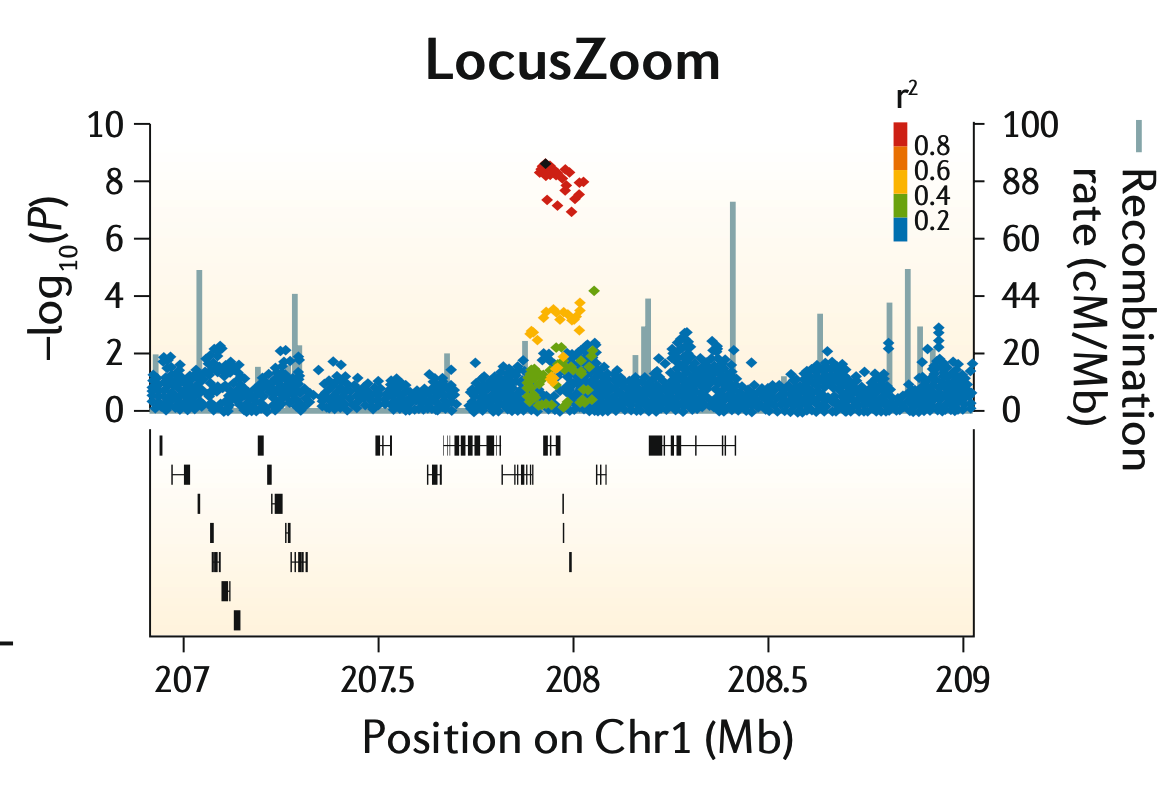
\includegraphics[width=3in]{./plots/zoom_in.png} 
   \caption{This figure  illustrates the patterns of association of each SNP with the lead SNP, as well as the annotation of genes in the region. Source: \cite{schaid2018genome}  }
   \label{fig:example}
\end{figure}
\end{column}%
\hfill%
\begin{column}{.30\textwidth}
\fontsize{7pt}{7pt}
\begin{block}{\small GWAS}
\begin{itemize}
\item Collect trait and genotypes (imputed)
\end{itemize}
\end{block}
\begin{block}{\small Marginal association of SNPs}
\begin{itemize}
\item Run linear mixed models or generalized mixed models 
\item Summarize results in Manhattan plot
\end{itemize}
\end{block}
\begin{block}{\small Investigate on independent locus}
\begin{itemize}
\item List of associated SNPs
\item Explore each independent regions
\end{itemize}
\end{block}
\begin{block}{\small Linkage disequilibrium (LD)}
\begin{itemize}
\item The leading SNPs are correlated to neighboring SNPs through LD
\item Association does not imply causation 
\end{itemize}
\end{block}
\end{column}%
\end{columns}
}
%%%%%%%%%%%%%%%%%%%%%%%%%%%%%%%%%%%%%%%%%%%%%%%%%%%%%%%%%%%%%%%%%%%%%%%%%%%%%%%%%%%%%%
%%%%%%%%%%%%%%%%%%%%%%%%%%%%%%%%%%%%%
\frame[t]{%4
\frametitle{GWAS pipeline}
\fontsize{7pt}{7pt}
\begin{columns}[T] % align columns
\begin{column}{.66\textwidth}
\begin{figure}[htbp] %  figure placement: here, top, bottom, or page
   \centering
   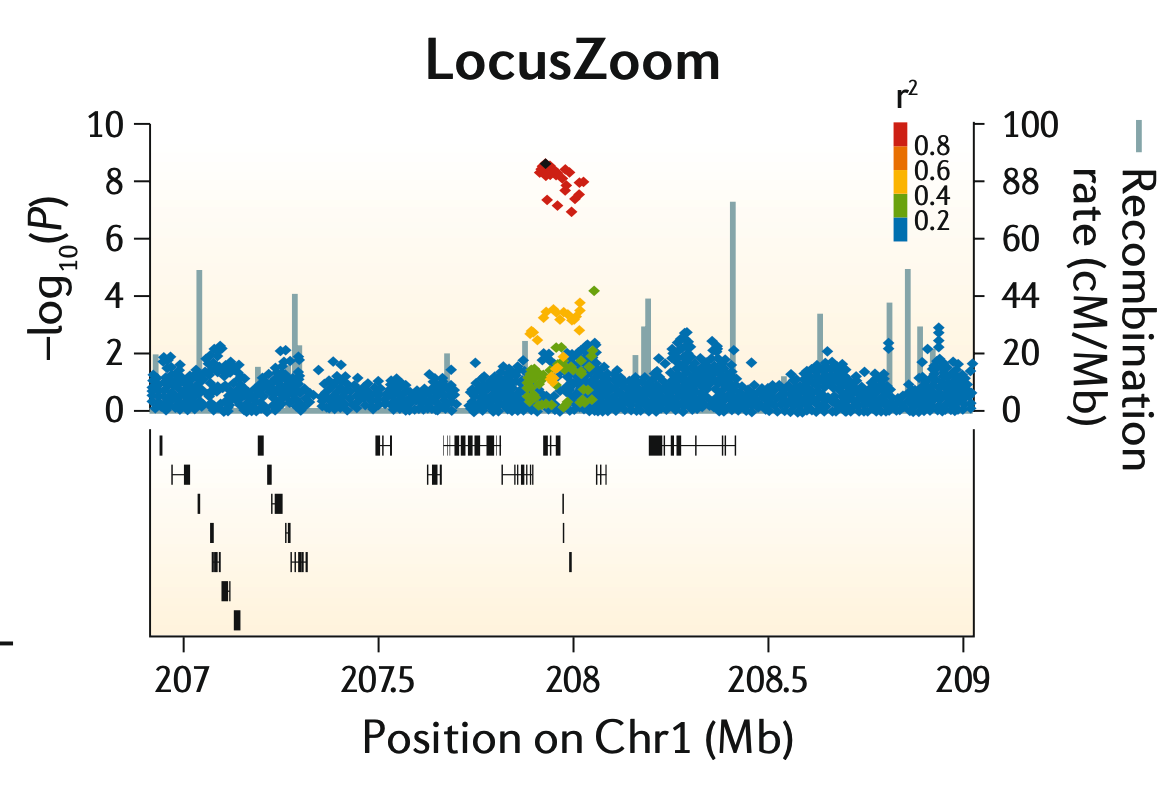
\includegraphics[width=3in]{./plots/zoom_in.png} 
   \caption{This figure  illustrates the patterns of association of each SNP with the lead SNP. Source: \cite{schaid2018genome}  }
   \label{fig:example}
\end{figure}
\begin{block}{\small Goal of Bayesian fine-mapping}
Fine-mapping methods utilize the results of the {\bf marginal association test} (between individual genotypes and phenotype) to select and {\bf prioritize genetic variants} accounting for the {\bf complex LD structure} among variants. 
\end{block}
\end{column}%
\hfill%
\begin{column}{.30\textwidth}
\fontsize{7pt}{7pt}
\begin{block}{\small GWAS}
\begin{itemize}
\item Collect trait and genotypes (imputed)
\end{itemize}
\end{block}
\begin{block}{\small Marginal association of SNPs}
\begin{itemize}
\item Run linear mixed models or generalized mixed models 
\item Summarize results in Manhattan plot
\end{itemize}
\end{block}
\begin{block}{\small Investigate on independent locus}
\begin{itemize}
\item List of associated SNPs
\item Explore each independent regions
\end{itemize}
\end{block}
\begin{block}{\small Linkage disequilibrium (LD)}
\begin{itemize}
\item The leading SNPs are correlated to neighboring SNPs through LD
\item Association does not imply causation 
\end{itemize}
\end{block}
\end{column}%
\end{columns}
}
%%%%%%%%%%%%%%%%%%%%%%%%%%%%%%%%%%%%%%%%%%%%%%%%%%%%%%%%%%%%%%%%%%%%%%%%%%%%%%%%%%%%%%

%%%%%%%%%%%%%%%%%%%%%%%%%%%%%%%%%%%%%%%%%%%%%%%%%%%%%%%%%%%%%%%%%%%%%%%%%%%%%%%%%%%%%%
\frame[t]{
\frametitle{Data structure of fine-mapping methods}

Due to logistic concerns and the availability of meta-analysis, researchers use and share summary statistics and LD matrix instead of directly using phenotype and genotype (large file size). 
\begin{block}{The marginal association test}
\begin{itemize}
\item In a given genomic region (Locus), there are $p$ variants and $n$ subjects. 
\item Let $\boldsymbol Z$ denote a $p$-dimensional vector, where $Z_i$ is the summary statistics of the  marginal test between the $i$th variant, $i=1,\ldots,p$ and the phenotype $(\boldsymbol y)$.
\item  The sampling distribution of $\boldsymbol Z$ can be written as:
 $$
 \boldsymbol Z| \boldsymbol\lambda,\sigma^2_y,\boldsymbol\Sigma \sim\text{MVN}(\boldsymbol\Sigma\boldsymbol\lambda,\sigma^2_y\boldsymbol\Sigma), 
$$
 where $\boldsymbol{\Sigma}$ is the LD correlation matrix of the variants in the given region.
 \item We assume $\boldsymbol \lambda$ is a sparse vector, and want to identify non-zero entries of  $\boldsymbol \lambda$ associated with the causal variants. 
\end{itemize}
\end{block}
}
%%%%%%%%%%%%%%%%%%%%%%%%%%%%%%%%%%%%%%%%%%%%%%%%%%%%%%%%%%%%%%%%%%%%%%%%%%%%%%%%%%%%%%
\frame[t]{
\frametitle{Challenges of genetic data}
\fontsize{7pt}{7pt}
\begin{block}{\small Complex LD structure}
 High and complex correlations among variants (i.e., high linkage disequilibrium (LD)).
\begin{figure}[H] %  figure placement: here, top, bottom, or page
   \centering
  
%\begin{tabular}{cc}
   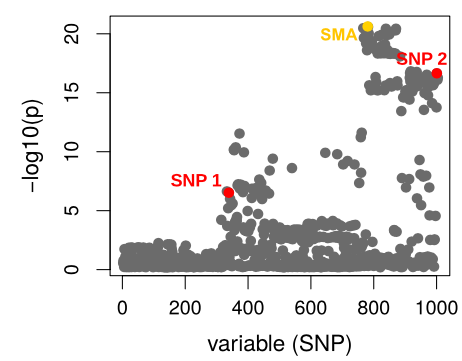
\includegraphics[width=1.5in]{plots/example_2.png} 
    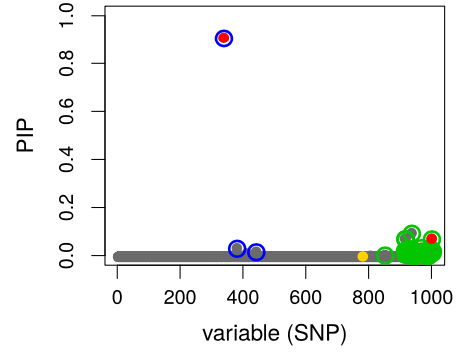
\includegraphics[width=1.5in]{plots/example_1.png} 
       \caption{The SNP ($\color{yellow}\bullet$) is not causal but  moderately correlated to the causal SNPs ($\color{red}\bullet$). \cite{wang2019simple}}
%   \end{tabular}
 \end{figure}~\\
\pause
\end{block}
\begin{block}{\small Highly correlated variants}
The causal variants could be highly correlated up to tens or even hundreds of other variants with very similar Z-scores. How to distinguish causal SNP from other highly correlated ones.
\end{block}
\pause
\begin{block}{\small Mismatch between $\boldsymbol Z$/LD due to meta-analysis}
\begin{itemize}
\item[$\boldsymbol Z$] To increase power, $\boldsymbol Z$ is often generated by the meta-analysis, where the sample size of generating individual Z-score can be dramatically different.
\item[$\Sigma$] To avoid transform the in-sample LD matrix of very large file size, $\Sigma$ is usually  extracted from reference panels, e.g., 1000G Genomes.
\item This creates inconsistencies between $\boldsymbol Z$/LD.
\end{itemize}
\end{block}
}
%%%%%%%%%%%%%%%%%%%%%%%%%%%%%%%%%%%%%%%%%%%%%%%%%%%%%%%%%%%%%%%%%%%%%%%%%%%%%%%%%%%%%%

%%%%%%%%%%%%%%%%%%%%%%%%%%%%%%%%%%%%%%%%%%%%%%%%%%%%%%%%%%%%%%%%%%%%%%%%%%%%%%%%%%%%%%
\frame[t]{
\frametitle{CARMA}
\fontsize{7pt}{7pt}
\begin{block}{\small Prior on effect size (coefficient)} 
 The sampling distribution of $\boldsymbol Z$ is:
 \begin{eqnarray*}
 \boldsymbol Z| \boldsymbol\lambda,\sigma^2_y,\boldsymbol\Sigma &\sim&\text{MVN}(\boldsymbol\Sigma\boldsymbol\lambda,\sigma^2_y\boldsymbol\Sigma).
  \end{eqnarray*}
  \begin{itemize}
 \item  Let $\boldsymbol\gamma'=\lrc{0,1}^p$ denote an indicator vector, such that $\gamma_i=1$ iff $\lambda_i\neq0$.
 \item  Let $S$ denote an index set such that $i\in S$ if $\gamma_i=1$.
 \item  $\boldsymbol \gamma_S$ and $M_S$ uniquely define a candidate model.  
 \item Given $S$, 
 the prior distribution of the assumed non-zero effect sizes $\boldsymbol\lambda_{\boldsymbol\gamma_S}$ that is associated with $\boldsymbol\gamma_S$ is 
\begin{eqnarray*}
\boldsymbol\lambda_{\boldsymbol\gamma_S}|{\sigma^2_y}, \tau, \boldsymbol\gamma_S&\sim&\text{MVN}(0, \frac{\sigma^2_y}{\tau}\boldsymbol\Sigma_{\boldsymbol\gamma_S}^{-1} ),\\
\tau&\sim& \text{Gamma}(\frac{1}{2},\frac{1}{2}),\\
\sigma^2_y&\sim&\frac{1}{\sigma^2_y}.\\
\lambda_i&=&0\text{ if }{\gamma_i=0}.
\end{eqnarray*}
\end{itemize}
\textbf{Remark:} CARMA is the first model introduce heavy-tailed prior distribution on the effect size (coefficients) in the fine-mapping setting, higher the power and smaller the size of the identified causal variants. 
\end{block}
\begin{block}{\small PIP}
We are interested in the posterior inclusion probability (PIP), i.e. $\Prob{\gamma_i=1|\boldsymbol Z, \boldsymbol \Sigma}.$\\ 
\end{block}
}

%%%%%%%%%%%%%%%%%%%%%%%%%%%%%%%%%%%%%%%%%%%%%%%%%%%%%%%%%%%%%%%%%%%%%%%%%%%%%%%%%%%%%%
%%%%%%%%%%%%%%%%%%%%%%%%%%%%%%%%%%%%%%%%%%%%%%%%%%%%%%%%%%%%%%%%%%%%%%%%%%%%%%%%%%%%%%

%%%%%%%%%%%%%%%%%%%%%%%%%%%%%%%%%%%%%%%%%%%%%%%%%%%%%%%%%%%%%%%%%%%%%%%%%%%%%%%%%%%%%%
%%%%%%%%%%%%%%%%%%%%%%%%%%%%%%%%%%%%%%%%%%%%%%%%%%%%%%%%%%%%%%%%%%%%%%%%%%%%%%%%%%%%%%
\frame[t]{
\frametitle{Dimensional penalization}
\fontsize{7pt}{7pt}
\begin{block}{Model space}%{Prior on $\boldsymbol \gamma$}
\begin{itemize}
\item Fine-mapping is intrinsically  a model selection problem in an ultra-sparse scenario.
\item Require dimensional penalization from the model space to control FDR.
\item Surprisingly, it has not been formally addressed by the previous fine-mapping methods, i.e. using the naive prior $\Prob{\gamma_i=1}=\frac{1}{p}$.
\end{itemize}
\end{block}
\pause
\begin{block}{Prior on Model space in CARMA}
\begin{itemize}
\item We introduce a prior distribution  on model space to control the total number of causal SNPs that any candidate model assumes
\item For a given model $M_S$, let $|S|=\sum_{\gamma_i\in{\boldsymbol\gamma}_S} \gamma_i$ denote the total number of causal SNPs for a given $\boldsymbol \gamma_S$ (dimension of $M_S$), we assign 
\[
|S||\eta\sim \text{Truncated Poisson}(\eta)\text{, for  $|S|\in\lrc{0,\ldots,p}$},
\]
which is first proposed in \cite{womack2015model}.
\item Then, for a specific model $\boldsymbol \gamma_S$ or $M_S$, the prior probability of  $\boldsymbol\gamma_S$ is
\begin{equation*}
\Prob{\boldsymbol\gamma_S|\eta}=\frac{\Prob{|S| |\eta}}{{p\choose |S|}}.
\end{equation*}
\item Another goal is  to identify the true model ($\boldsymbol \gamma_T$ or $M_T$) that generated the summary statistics, through posterior inference within a Bayesian paradigm. 
The model selection consistency  is shown in \cite{castillo2012needles,womack2015model}.
\end{itemize}
\end{block}
}
%%%%%%%%%%%%%%%%%%%%%%%%%%%%%%%%%%%%%%%%%%%%%%%%%%%%%%%%%%%%%%%%%%%%%%%%%%%%%%%%%%%%%%
\frame[t]{
\frametitle{Computation of PIP}
\fontsize{7pt}{7pt}
\begin{block}{}
\begin{itemize}
\item Let $\mathcal{M}$ denote the model set that contains all candidate models. 
\item Then \begin{itemize}
\item the posterior probability of any non-null model $\boldsymbol\gamma_S$ \item the posterior probability  of $\gamma_i$ being equal to 1 (PIP)
\end{itemize} can be computed as 
 \begin{align*}
 \Prob{\boldsymbol\gamma_S|\boldsymbol Z}&=\frac{PO_{\boldsymbol\gamma_S:\boldsymbol\gamma_0}}{\sum_{\boldsymbol\gamma_A\in \mathcal{M}}PO_{\boldsymbol\gamma_A:\boldsymbol\gamma_0}},\\
 \Prob{\gamma_i=1|\boldsymbol Z}&=\sum_{\boldsymbol\gamma_{S}:i\in S}  \Prob{\boldsymbol\gamma_S|\boldsymbol Z},
 \end{align*}
 where the posterior odds ($PO_{\boldsymbol\gamma_S:\boldsymbol\gamma_0}$) is defined as the product of the Bayes factor $\lrp{\frac{f(\boldsymbol Z|\boldsymbol\gamma_S)}{f(\boldsymbol Z|\boldsymbol\gamma_0)}}$ and the prior odds $\lrp{\frac{\Prob{\boldsymbol\gamma_S|\eta}}{\Prob{\boldsymbol\gamma_0|\eta}}}$:
 \begin{align*}
PO_{\boldsymbol\gamma_S:\boldsymbol\gamma_0}&=\frac{f(\boldsymbol Z|\boldsymbol\gamma_S)}{f(\boldsymbol Z|\boldsymbol\gamma_0)} \frac{\Prob{\boldsymbol\gamma_S|\eta}}{\Prob{\boldsymbol\gamma_0|\eta}}\\
&=\frac{\eta^{|S|}(p-|S|)!}{p!}\int_0^\infty  \lrb{1-\frac{ \boldsymbol Z_S'{\boldsymbol\Sigma_{\boldsymbol\gamma_S}^{-1}}\boldsymbol Z_S  }{ \boldsymbol Z'\boldsymbol\Sigma^{-1}\boldsymbol  Z\lrp{1+\tau}}}^{-\frac{p}{2}} \lrp{\frac{1+\tau}{\tau}}^{-\frac{|S|}{2}}  f(\tau)\d\tau.
\end{align*}
\end{itemize}
\end{block}
}

%%%%%%%%%%%%%%%%%%%%%%%%%%%%%%%%%%%%%%%%%%%%%%%%%%%%%%%%%%%%%%%%%%%%%%%%%%%%%%%%%%%%%%
\frame[t]{
\frametitle{Computation algorithm}
\fontsize{7pt}{7pt}
\begin{block}{\small Drawbacks of previous methods}
\begin{itemize}
\item  There are $2^p$ candidate models. Impossible to going over all models.
\item  Exhaustively screening $\Prob{\boldsymbol Z|\Sigma, \boldsymbol \gamma}$ for all $\lrc{\boldsymbol \gamma;\sum\boldsymbol \gamma<\#}$ with a restriction on $\#$ (e.g.$\#=2$) is very slow and restrictive.
\item Stochastic search (MCMC) is also slow and requiring restriction on $\sum\boldsymbol \gamma$, and exploring posterior model space unevenly for highly correlated variants. 
\end{itemize}
\end{block}
\begin{block}{\small Shotgun algorithm \cite{hans2007shotgun}}
\begin{itemize}
\item Given a specific model denoted by an index set $S$, say $S=\lrc{1,2,3}$,  the Shotgun algorithm is  an iterative procedure that  exhaustively examines the neighborhood of the current model, defined as:
\begin{align*}
\Gamma_{-}(S)&:=\lrc{A:A\subset S, |S|-|A|=1} \textrm{(one less variable than $S$)},\\
\Gamma_{+}(S)&:=\lrc{A:A\supset A, |A|-|S|=1} \textrm{(one more variable than $S$)},\\
\Gamma_{\Leftrightarrow}(S)&:=\lrc{A:|S|-|A \cap S|=1, |A|=|S|} \textrm{(models that replaces one variable in $S$)}.
\end{align*}
\item To update the current model, the algorithm selects one candidate model from $\Gamma_{-}(S)$, $\Gamma_{+}(S)$, and $\Gamma_{\Leftrightarrow}(S)$ according to the corresponding  posterior probabilities, i.e. $\Prob{M_A|\boldsymbol Z}$.

\end{itemize}
\end{block}
\begin{block}{\small Advantages of Shotgun}
\begin{itemize}
\item  Semi-exhaustive searching, evenly exploring the group of highly correlated variables. 
\item  Stochastically moves towards the high posterior area in the model space.
\end{itemize}
\end{block}
}

%%%%%%%%%%%%%%%%%%%%%%%%%%%%%%%%%%%%%%%%%%%%%%%%%%%%%%%%%%%%%%%%%%%%%%%%%%%%%%%%%%%%%%
%%%%%%%%%%%%%%%%%%%%%%%%%%%%%%%%%%%%%%%%%%%%%%%%%%%%%%%%%%%%%%%%%%%%%%%%%%%%%%%%%%%%%%
\frame[t]{
\frametitle{Incorporating functional annotations}
\fontsize{7pt}{7pt}
\begin{block}{\small Motivation}
\fontsize{7pt}{7pt}
\begin{itemize}
\item  There are abundant information of the causality of SNPs from the external resource, i.e. functional annotations (gene expression (eQTL)).
\item  We want to use annotations to distinguish causal variants from highly correlated non-causal variants. 
\end{itemize}
\end{block}
\begin{block}{\small Strategy of EM-algorithm}
\begin{itemize}
\item  By adding the functional annotations, the likelihood can be written as:
\begin{align*}
L(\boldsymbol \theta;\boldsymbol Z,\boldsymbol \gamma, W)&=f(\boldsymbol Z|\boldsymbol\gamma)\Prob{\boldsymbol\gamma|W,\boldsymbol \theta},
\end{align*} 
where $W$ is the matrix of annotations and $\boldsymbol \theta$ is the corresponding coefficients. 
\item Using EM algorithm to maximize likelihood, which associates $\boldsymbol\gamma$ and $W$ with a Poisson regression. 
\item {\bf Feature selection on functional annotations.}  By introducing the elastic net penalty, CARMA can perform variable selection  on the potentially high-dimensional functional annotation data. 
\item {\bf Multiplicity control.} CARMA associates the Poisson regression to the Poisson prior on model space. 
\end{itemize}
\end{block}


}

%%%%%%%%%%%%%%%%%%%%%%%%%%%%%%%%%%%%%%%%%%%%%%%%%%%%%%%%%%%%%%%%%%%%%%%%%%%%%%%%%%%%%%
%%%%%%%%%%%%%%%%%%%%%%%%%%%%%%%%%%%%%%%%%%%%%%%%%%%%%%%%%%%%%%%%%%%%%%%%%%%%%%%%%%%%%%
\frame[t]{
\frametitle{Outliers motivation}
\fontsize{7pt}{7pt}
\begin{figure}[htbp] %  figure placement: here, top, bottom, or page
   \centering
   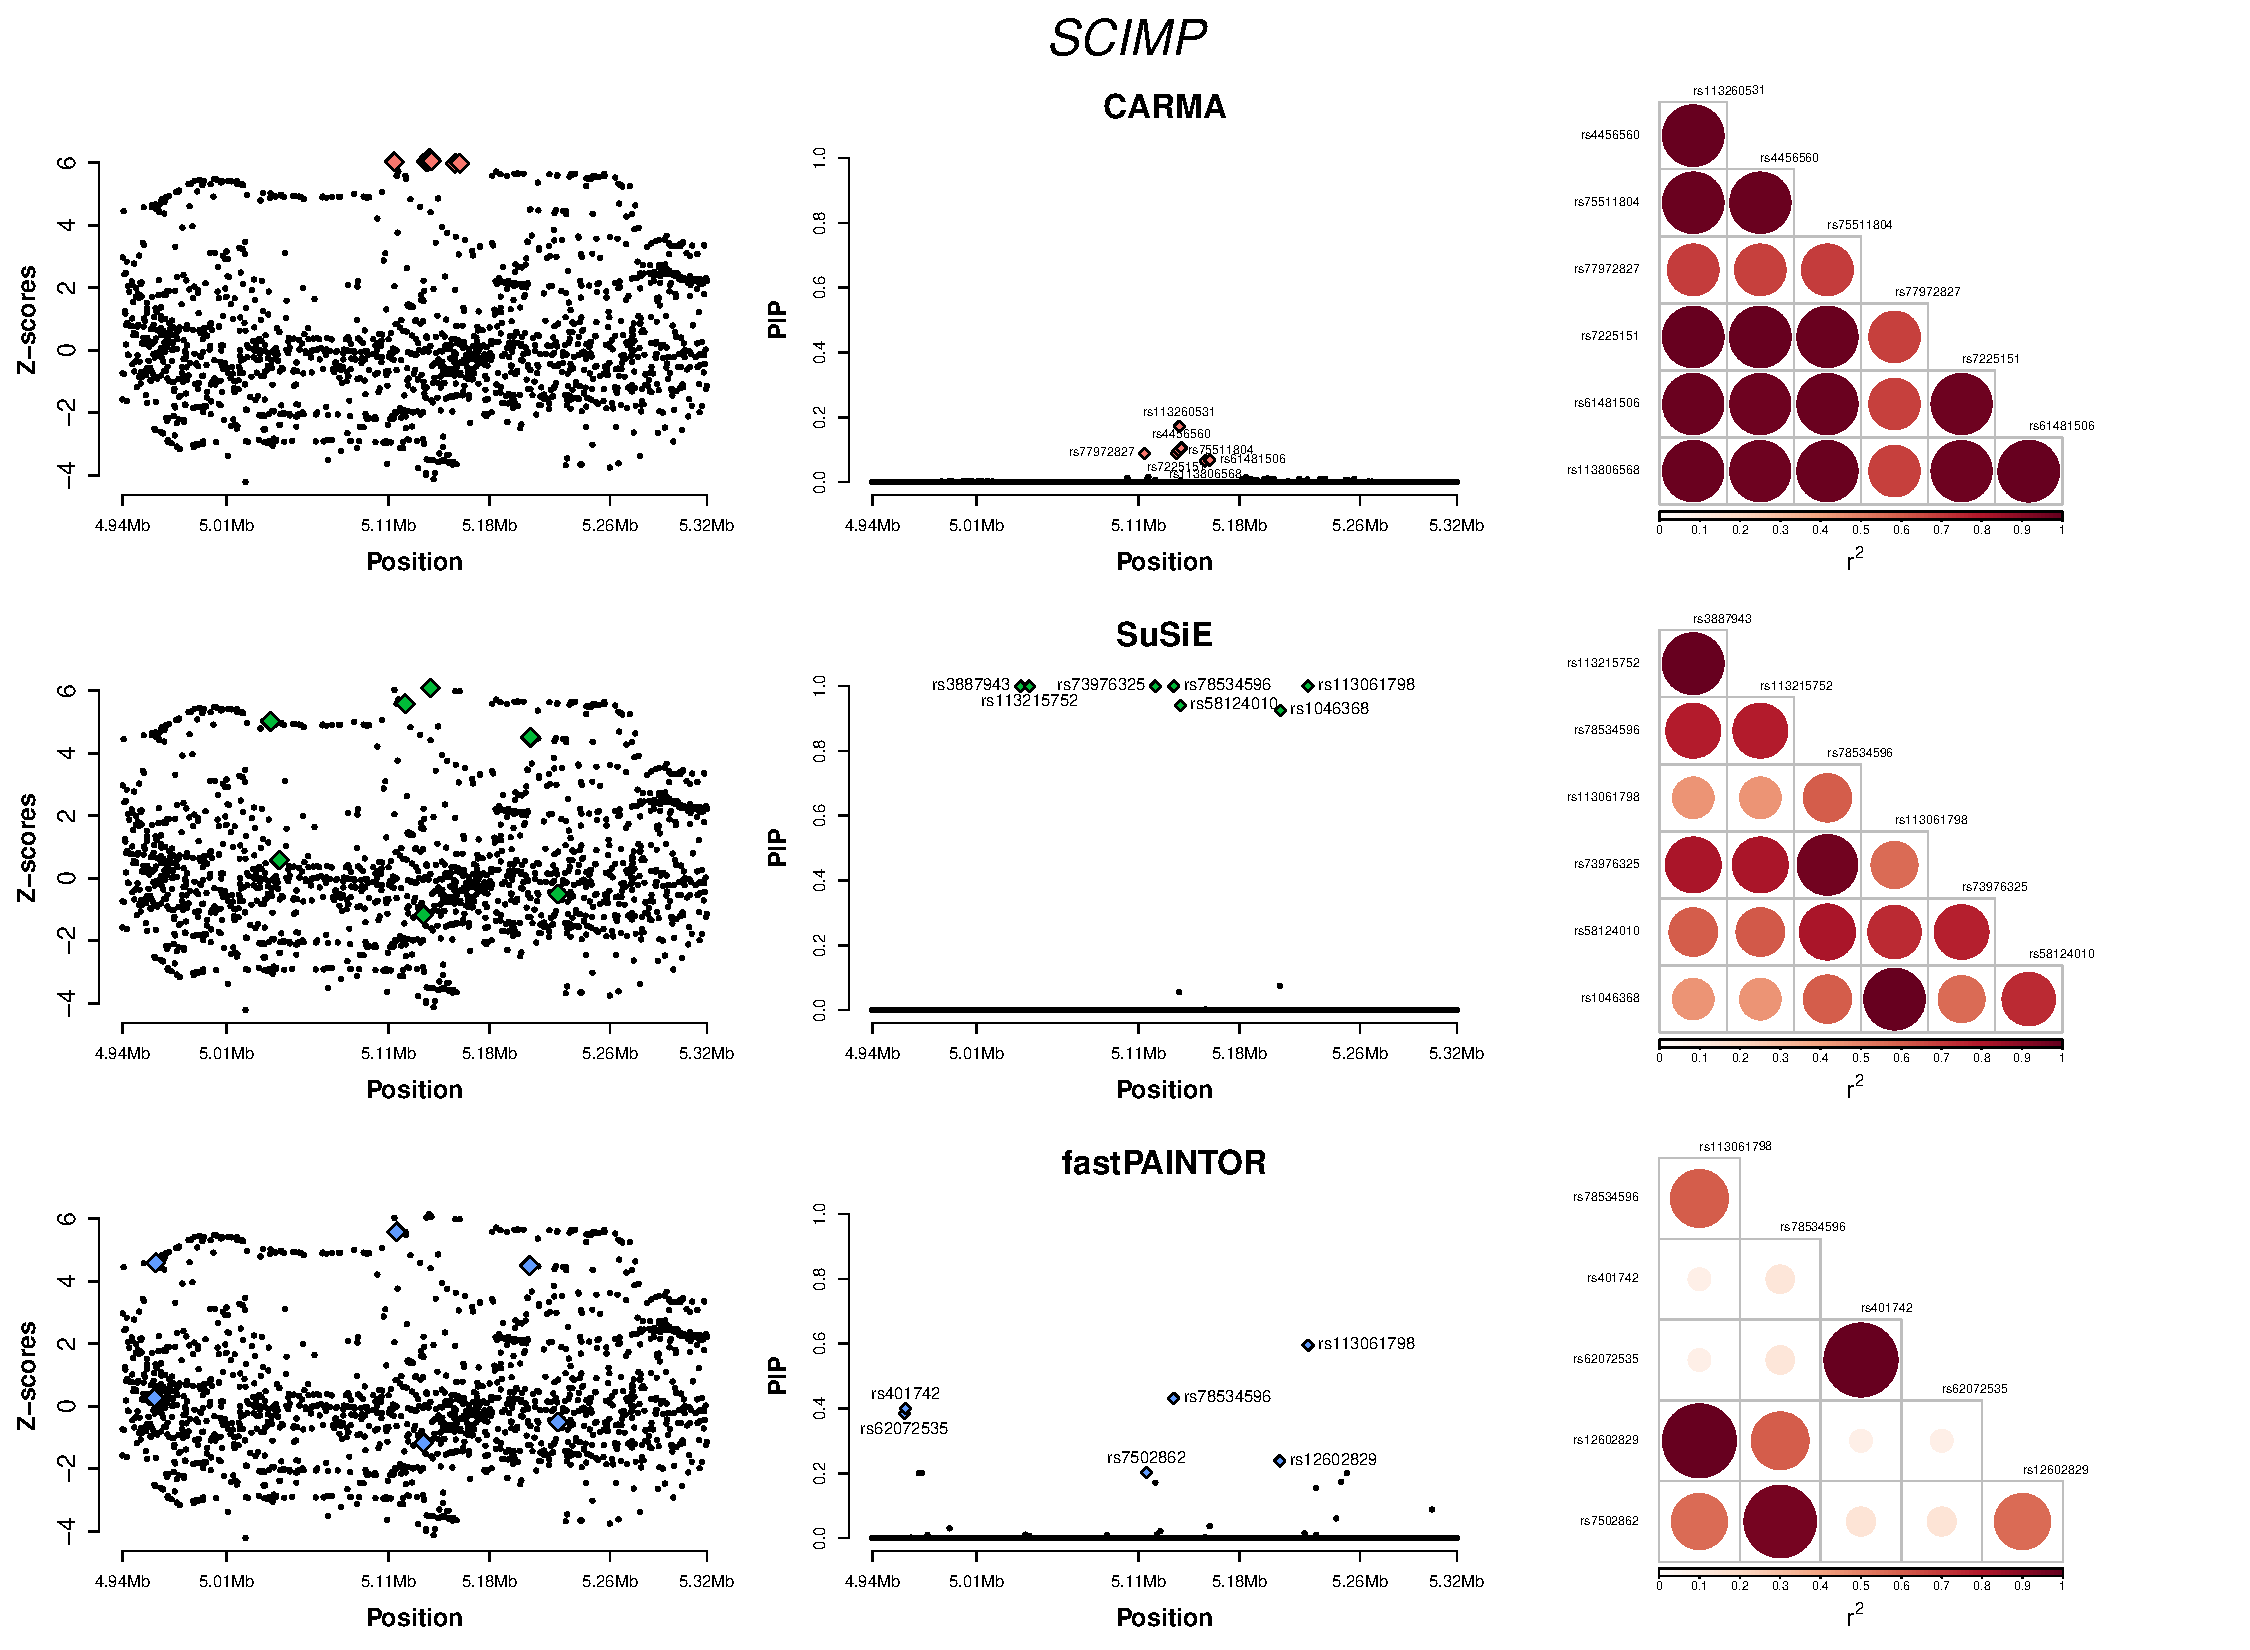
\includegraphics[width=4.5in]{./plots/AD_motivation_examplep_chr17_1_SCIMP_indi_r2_ld1.pdf} 
   \caption{{\bf Motivating example.} GWAS Z-scores along with PIPs from three models (CARMA, SuSiE and fastPAINTOR) for one Alzheimer's disease risk locus {\it SCIMP} (GRCh37/hg19)}
   \label{fig:example}
\end{figure}
}
\frame[t]{
\frametitle{Outliers in fine-mapping}
\begin{block}{\small Outlier detection}
\begin{itemize}
\item Let $\tilde{\boldsymbol Z}=\lrc{Z_1,\ldots,Z_{|D|}}'$ denote a group of highly correlated SNPs with $\text{cor}\lrp{Z_i,Z_j}\ge r_{\text{outlier}}$ ($r_{\text{outlier}}>0.9$), for $\forall i,j\in D$ 
\item We can assume that the random variable vector $\tilde{\boldsymbol Z}$ follow a MVN$\lrp{\mathbf{1}_{|D|}\beta,\boldsymbol\Sigma_D}$.
\item In a loop algorithm, we  test whether $Z_i$ is generated by a different distribution, i.e. $N(\beta,c)$:
\begin{align*}
H_0: c&=1; \text{ $Z_i$ is not an outlier}\\
 H_1: c&\neq1; \text{ $Z_i$ is an outlier}. 
\end{align*}
\item We assume $\tilde{\boldsymbol Z}_{-i}$ are not outliers  and follow a MVN$\lrp{\mathbf{1}_{|D|-i}\beta,\boldsymbol\Sigma_{D_{-i}}}$.
\item Computing the  Bayes factor between the two hypothesis and dropping the variants if reject $H_0$.
\end{itemize}
\end{block}
}
%%%%%%%%%%%%%%%%%%%%%%%%%%%%%%%%%%%%%%%%%%%%%%%%%%%%%%%%%%%%%%%%%%%%%%%%%%%%%%%%%%%%%%
%%%%%%%%%%%%%%%%%%%%%%%%%%%%%%%%%%%%%%%%%%%%%%%%%%%%%%%%%%%%%%%%%%%%%%%%%%%%%%%%%%%%%%
\frame[t]{
\frametitle{Credible set and credible model}
\fontsize{7pt}{7pt}
\begin{block}{\small Credible set}
\begin{itemize}
\item In \cite{wang2019simple} the authors define a credible set, and can be simplified as
 \begin{definition}
Given $\rho=0.99$ and a correlation threshold $r$, $S$ is a credible set of variants if 
\begin{itemize}
\item $\sum_{i \in S}\Prob{\gamma_i|\boldsymbol Z}\ge \rho$
\item $\text{min}\lrc{cor(i,j)\ge r},\text{ for all $i,j\in S$}$
\item $|S|$ is minimal. 
 \end{itemize}
 \end{definition}
 \item Credible sets can identify  groups of highly correlated variants for further experimental validations. 
\end{itemize}
\end{block}
\begin{block}{\small Credible Model}
\begin{itemize}
\item Instead of credible set, we propose the concept of  credible model.
\item  Let $\boldsymbol\gamma_{(b)}$, $b=1,\ldots,B$, denote the ranked candidate models, such as $\boldsymbol\gamma_{(1)}$ receives the largest marginal likelihood.
\item We use $\boldsymbol\gamma_{(1)}$ as the reference model to select all other candidate models.
\item Including any candidate models into the credible model such as 
\[
\text{PO}_{\boldsymbol\gamma_{(1)}:\boldsymbol\gamma_{(b)}}=\frac{\Prob{\boldsymbol\gamma_{(1)}|\boldsymbol Z,\eta}}{\Prob{\boldsymbol\gamma_{(b)}|\boldsymbol Z,\eta}}=\frac{\Prob{\boldsymbol Z|\boldsymbol\gamma_{(1)}}\Prob{\boldsymbol\gamma_{(1)}|\eta}}
{\Prob{\boldsymbol Z|\boldsymbol\gamma_{(b)}}\Prob{\boldsymbol\gamma_{(b)}|\eta}}<10.
\]
\end{itemize}
\end{block}

}

%%%%%%%%%%%%%%%%%%%%%%%%%%%%%%%%%%%%%%%%%%%%%%%%%%%%%%%%%%%%%%%%%%%%%%%%%%%%%%%%%%%%%%
%%%%%%%%%%%%%%%%%%%%%%%%%%%%%%%%%%%%%%%%%%%%%%%%%%%%%%%%%%%%%%%%%%%%%%%%%%%%%%%%%%%%%%
\frame[t]{
\frametitle{ Simulating genotype based on real data}
\fontsize{6pt}{7pt}
\begin{block}{\small Simulation settings }
\begin{itemize}
\item We use the R package `sim1000G' \cite{dimitromanolakis2019sim1000g} to simulate genotypes based on the 1000 Genomes Project data.
\item We focus on 94 loci identified as risk regions in a recent GWAS on breast cancer \cite{fachal2020fine}.
\item The number of variants in each region ranges between $\sim 1,500-4,000$. 
\item We simulate genotype data for $n=10,000$  individuals. 
\end{itemize}
\end{block}
\begin{block}{\small Prior probability}
\begin{itemize}
\item We use functional annotations (randomly select 200 chromatin features out of 919 DeepSEA  chromatin features \cite{zhou2015predicting}) to determine the causalities of variants, such as $\Prob{\gamma_i=1|\boldsymbol\theta,\boldsymbol w_i}=\frac{\exp{\boldsymbol w_i'\boldsymbol\theta}}{1+\exp{\boldsymbol w_i'\boldsymbol\theta}}$.
\item Let $T$ denote the index set of the  true causals selected, and $|T|=3$.
\end{itemize}
\end{block}
\begin{block}{\small Phenotype and summary statistics}
\begin{itemize}
\item For each $i \in T$, $\gamma_i=1$ and  $\beta_i\sim N(0,0.5^2)$.
\item The phenotypic variance $\sigma_y^2$ is computed such that $\phi=0.0075$, where 
 $\phi=\frac{\text{Var}(\boldsymbol X\boldsymbol\beta)}{\sigma_y^2+\text{Var}(\boldsymbol X\boldsymbol\beta)}.$
 \item Then we sample $\boldsymbol y$ such that $\boldsymbol y=\boldsymbol X\boldsymbol\beta+\boldsymbol\epsilon\text{; $\boldsymbol\epsilon\sim$ N(0, $\sigma_y^2I_{n\times n}$)}$. 
 \item Compute $\boldsymbol Z$ and $\boldsymbol \Sigma$.
 \item Two other very popular testing fine-mapping models, SuSiE\cite{wang2019simple} and fastPAINTOR\cite{kichaev2017improved}.
 \item We assume two  scenarios (1) no functional annotation and (2)  with functional annotations (919 DeepSEA  chromatin features).
\end{itemize}
\end{block}
}
%%%%%%%%%%%%%%%%%%%%%%%%%%%%%%%%%%%%%%%%%%%%%%%%%%%%%%%%%%%%%%%%%%%%%%%%%%%%%%%%%%%%%%
%%%%%%%%%%%%%%%%%%%%%%%%%%%%%%%%%%%%%%%%%%%%%%%%%%%%%%%%%%%%%%%%%%%%%%%%%%%%%%%%%%%%%%
\frame{
\frametitle{Simulation results (no outlier)}
\begin{figure}[htbp] %  figure placement: here, top, bottom, or page
   \centering
   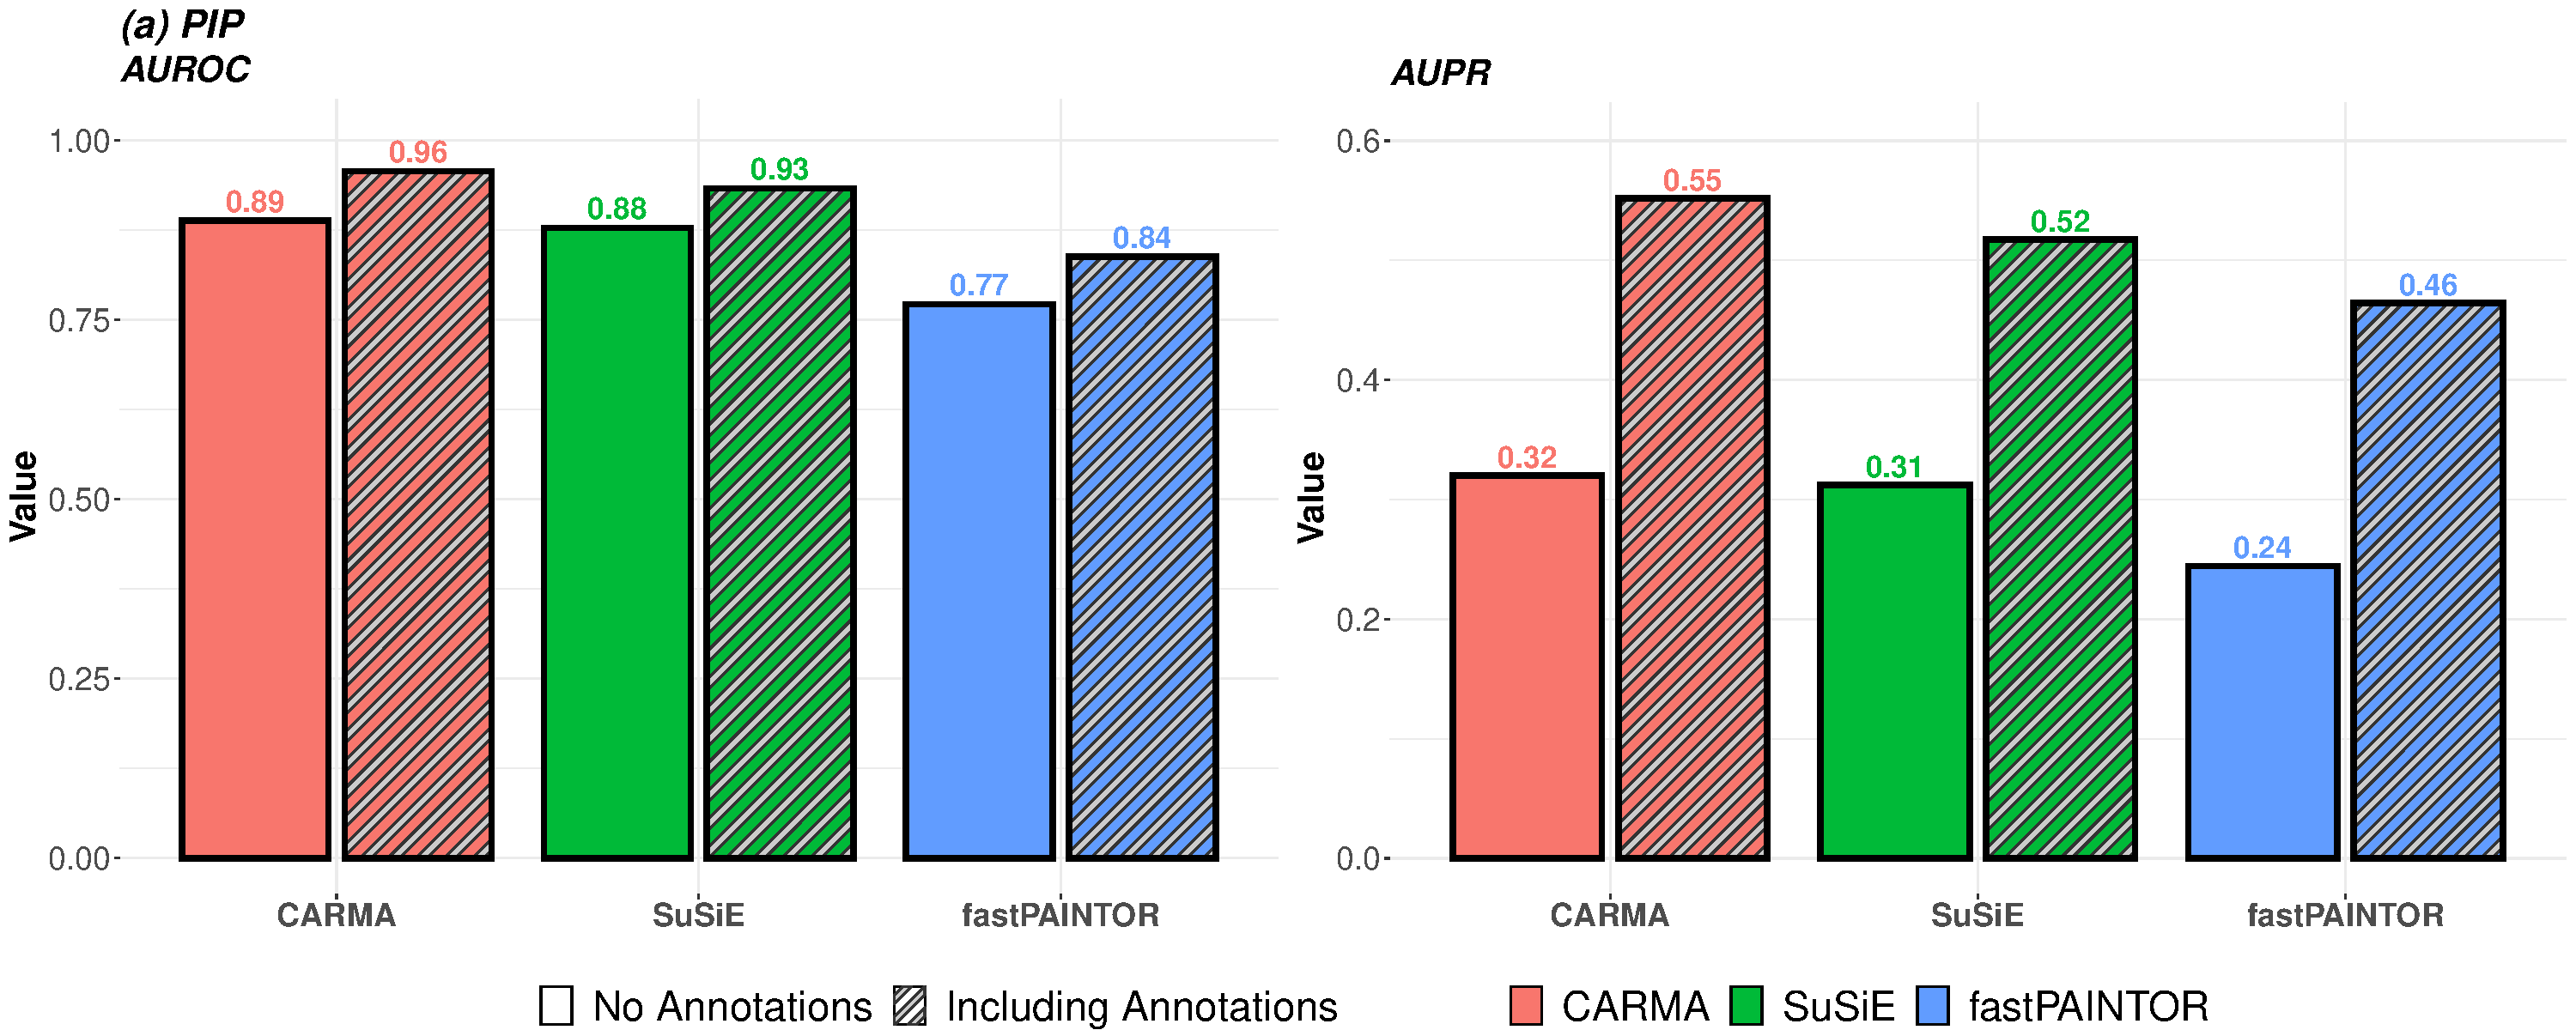
\includegraphics[width=4.5in]{./plots/normal_in-sample_AUPR_AUROC_|T|=3.pdf} 
%      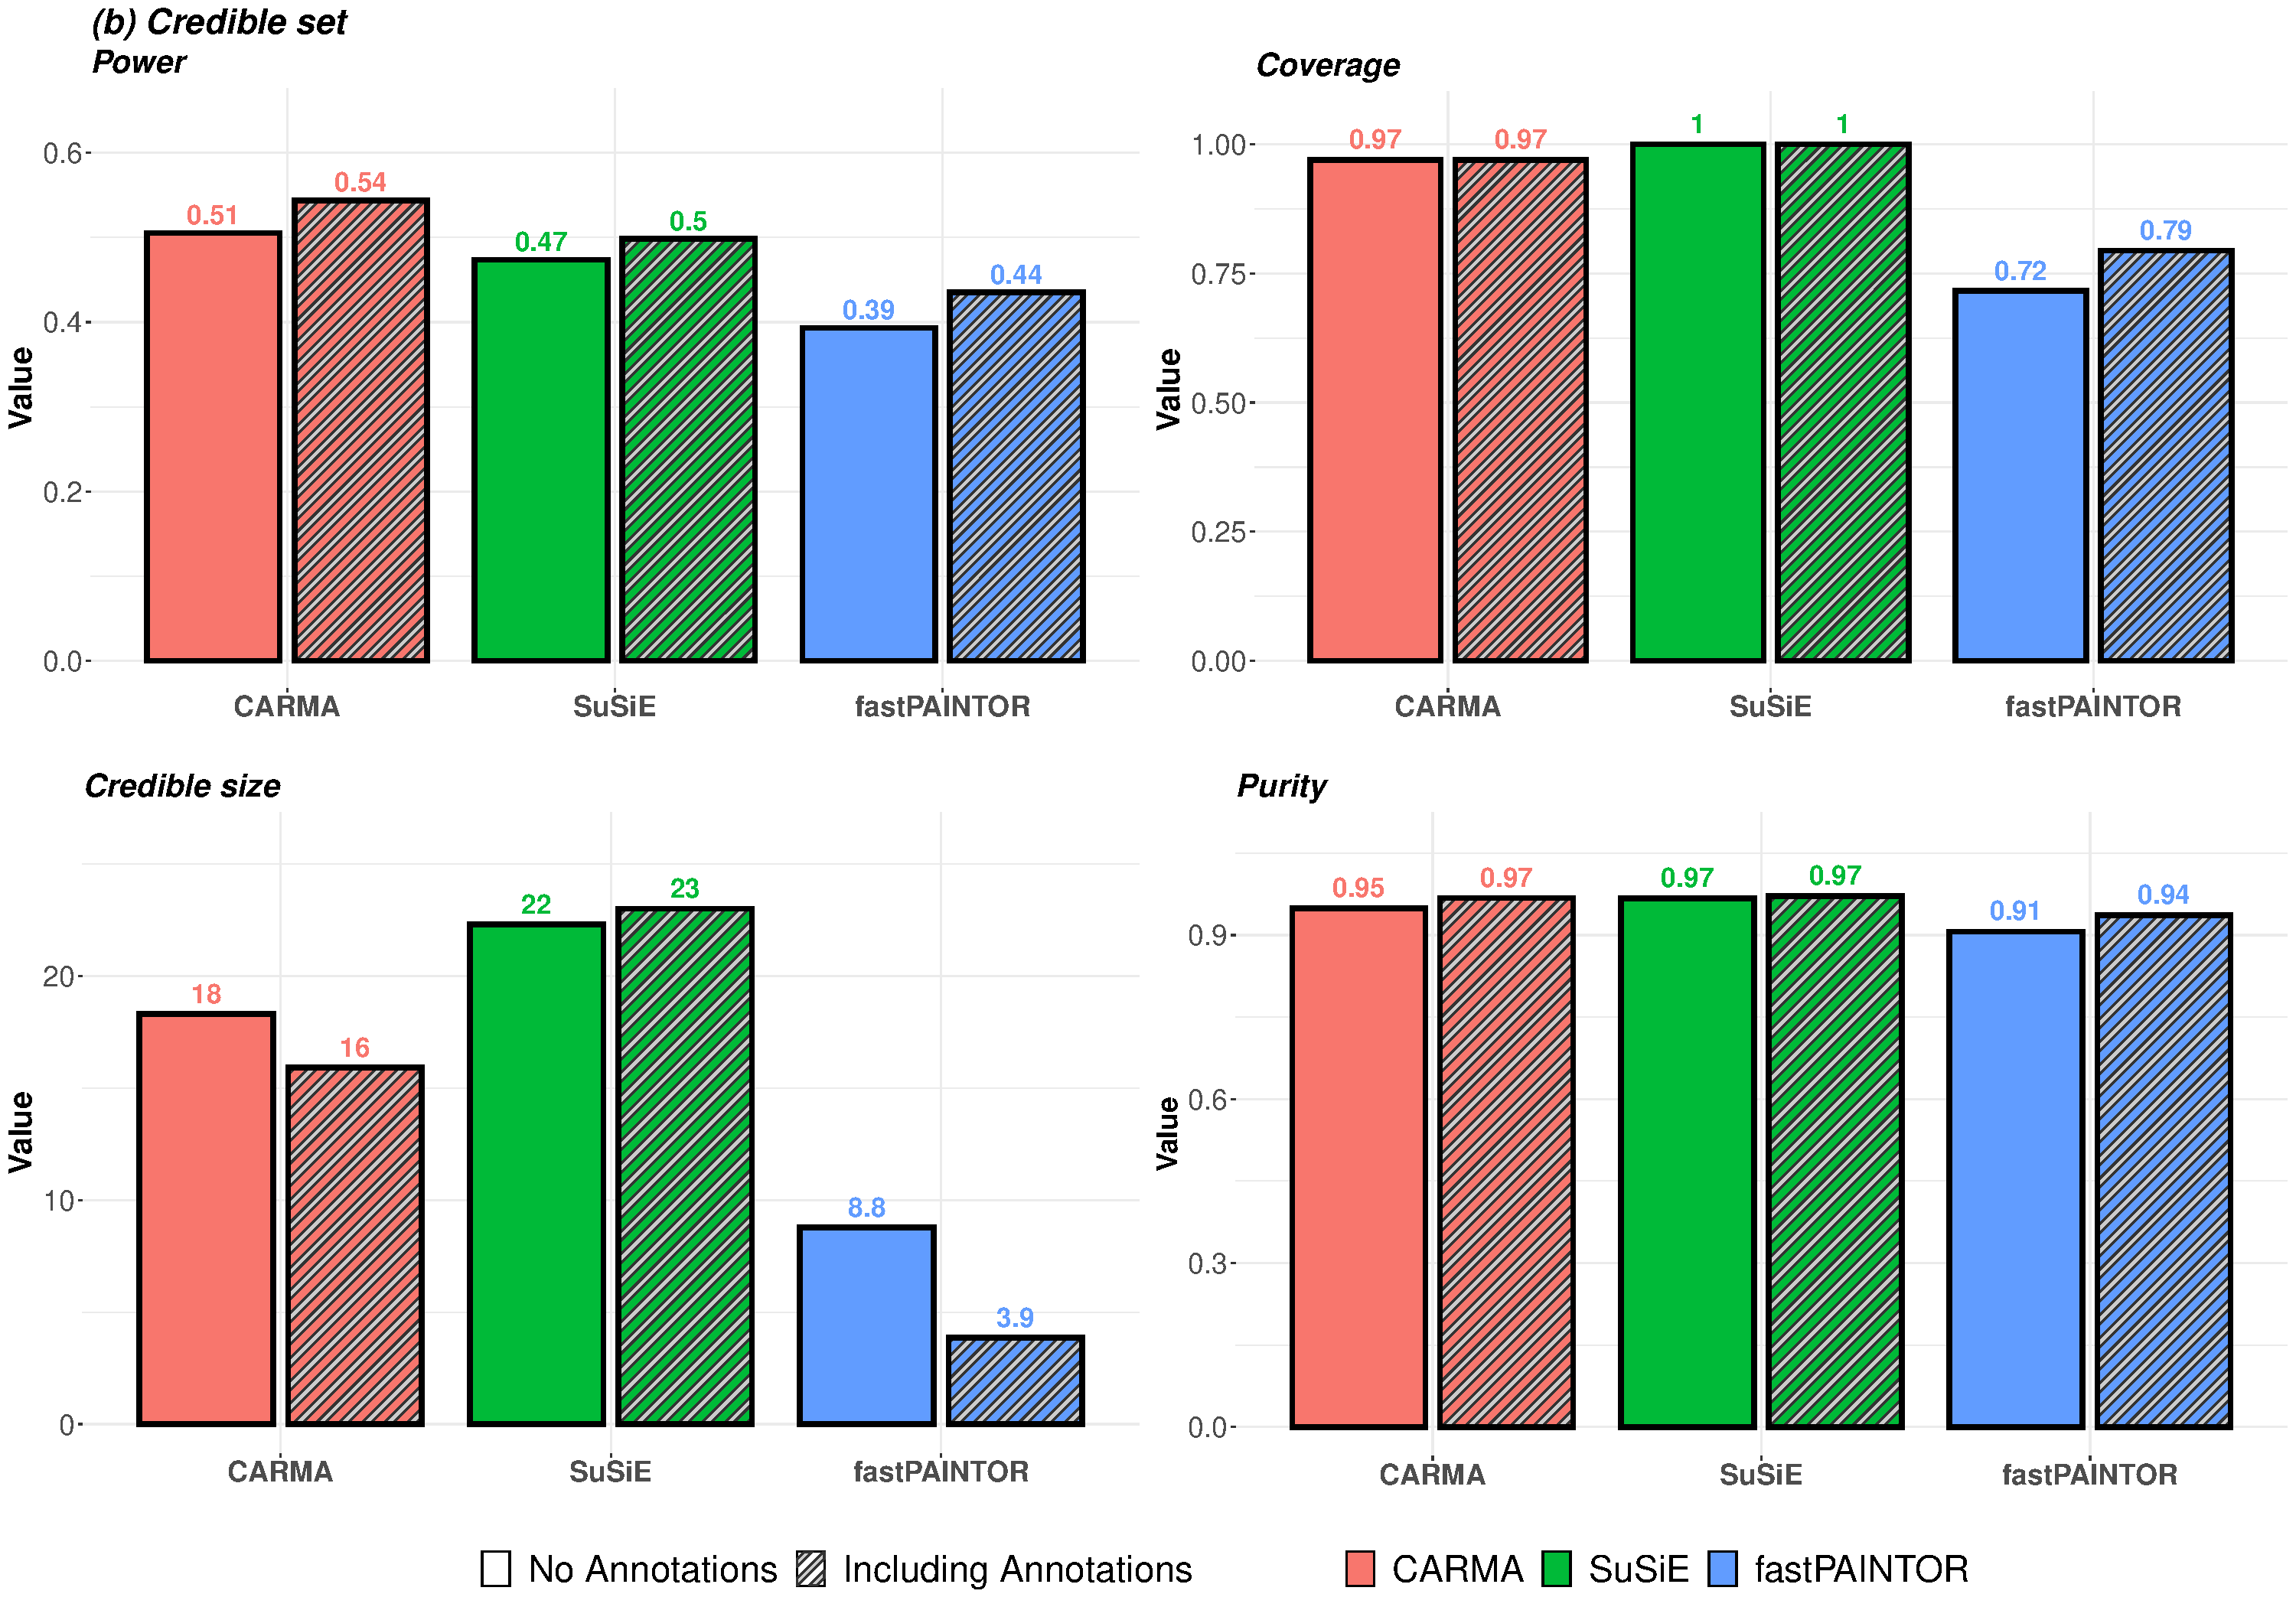
\includegraphics[width=2.5in]{./plots/normal_in-sample_credible_set_|T|=3.pdf} 
   \caption{AUROC and AUPR of the testing models}
   \label{fig:example}
\end{figure}
}
%%%%%%%%%%%%%%%%%%%%%%%%%%%%%%%%%%%%%%%%%%%%%%%%%%%%%%%%%%%%%%%%%%%%%%%%%%%%%%%%%%%%%%
%%%%%%%%%%%%%%%%%%%%%%%%%%%%%%%%%%%%%%%%%%%%%%%%%%%%%%%%%%%%%%%%%%%%%%%%%%%%%%%%%%%%%%
\frame{
\frametitle{Simulation results (no outlier)}
\begin{figure}[htbp] %  figure placement: here, top, bottom, or page
   \centering
%   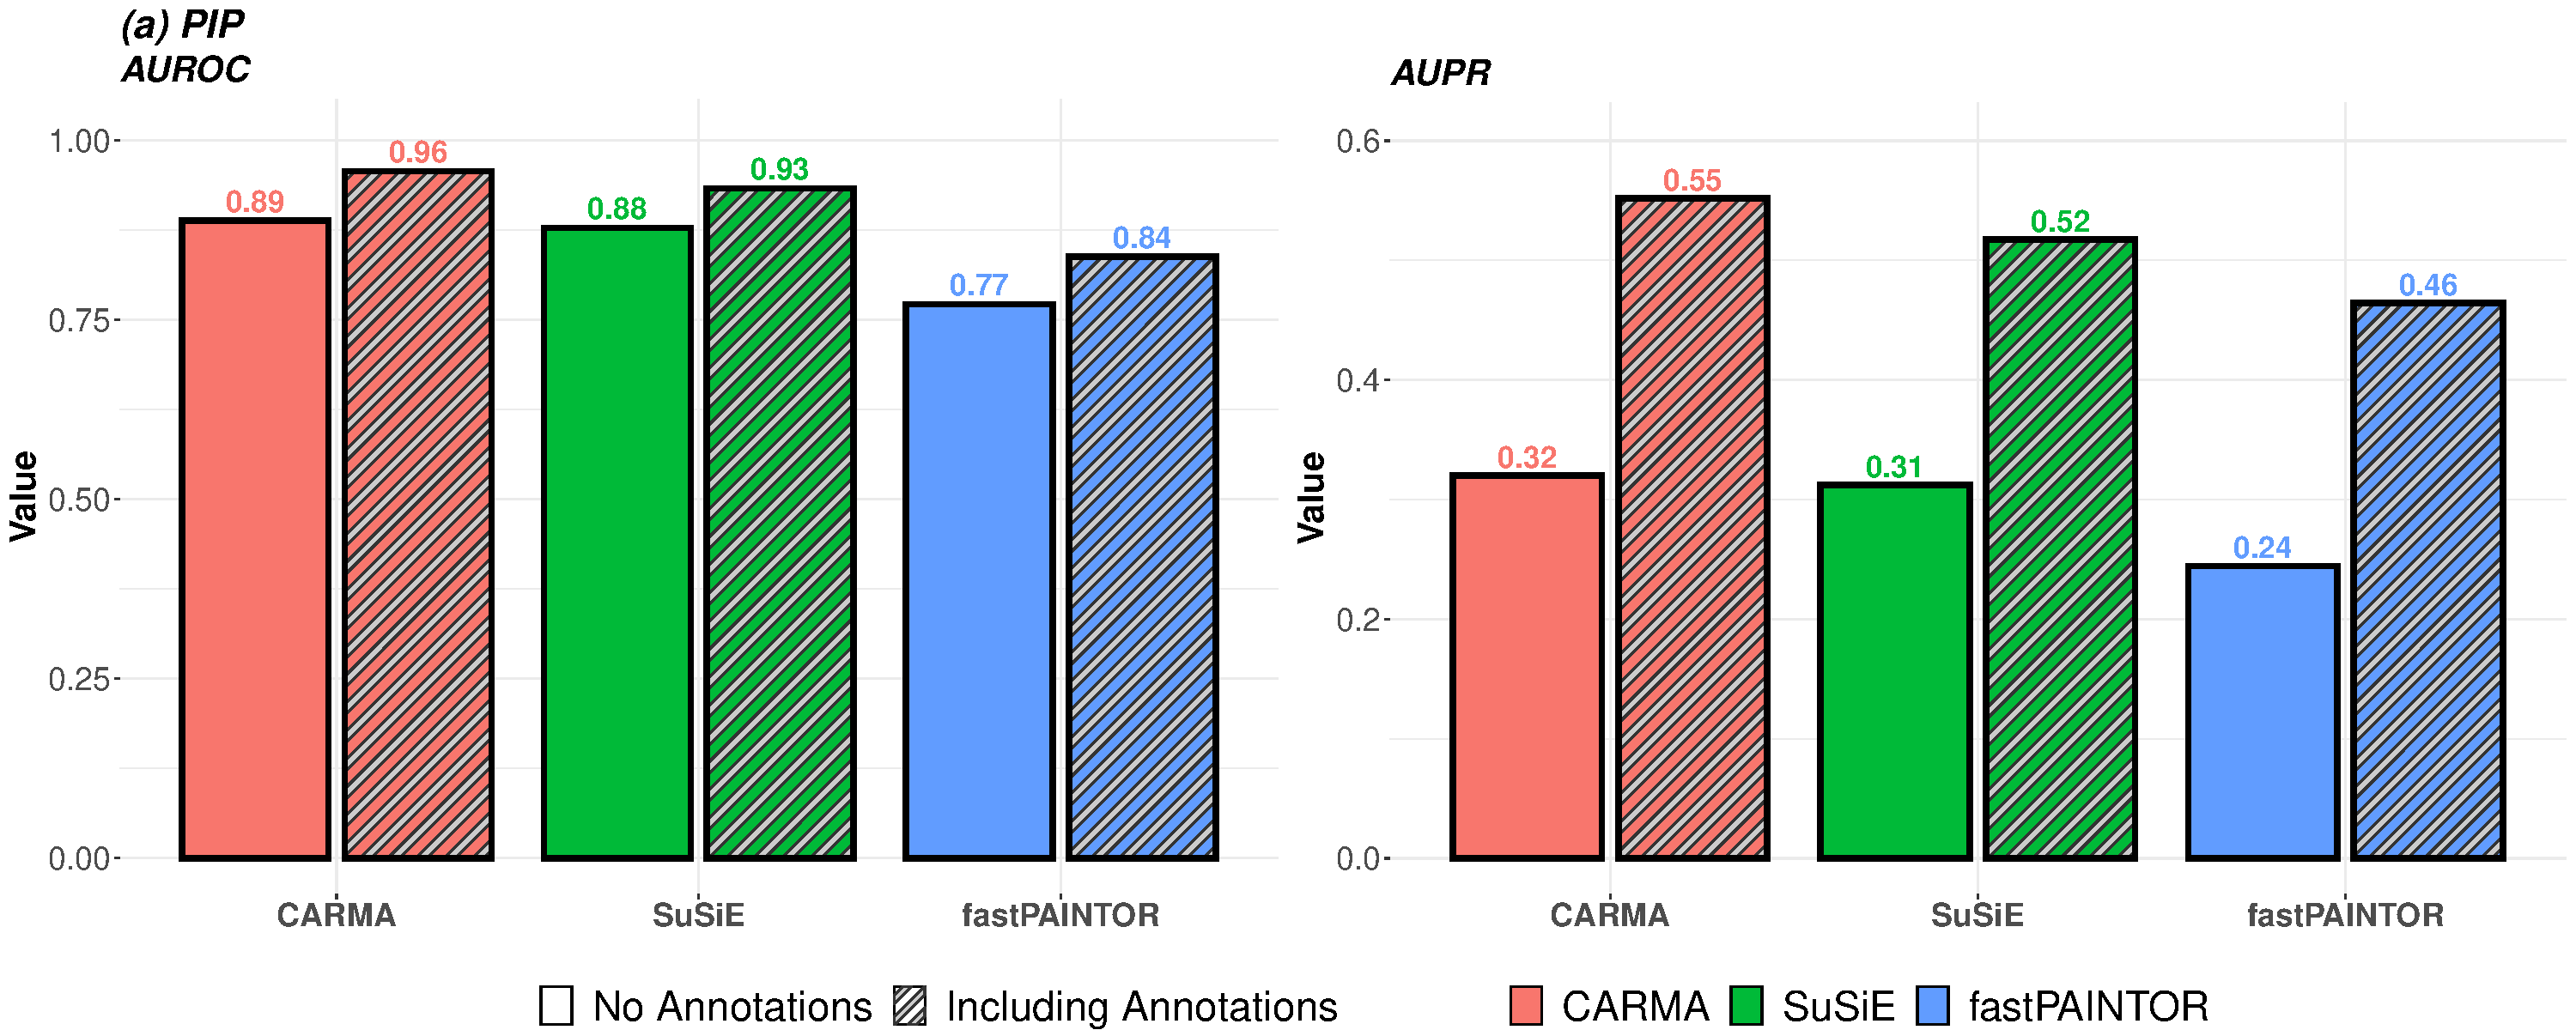
\includegraphics[width=2.5in]{./plots/normal_in-sample_AUPR_AUROC_|T|=3.pdf} 
      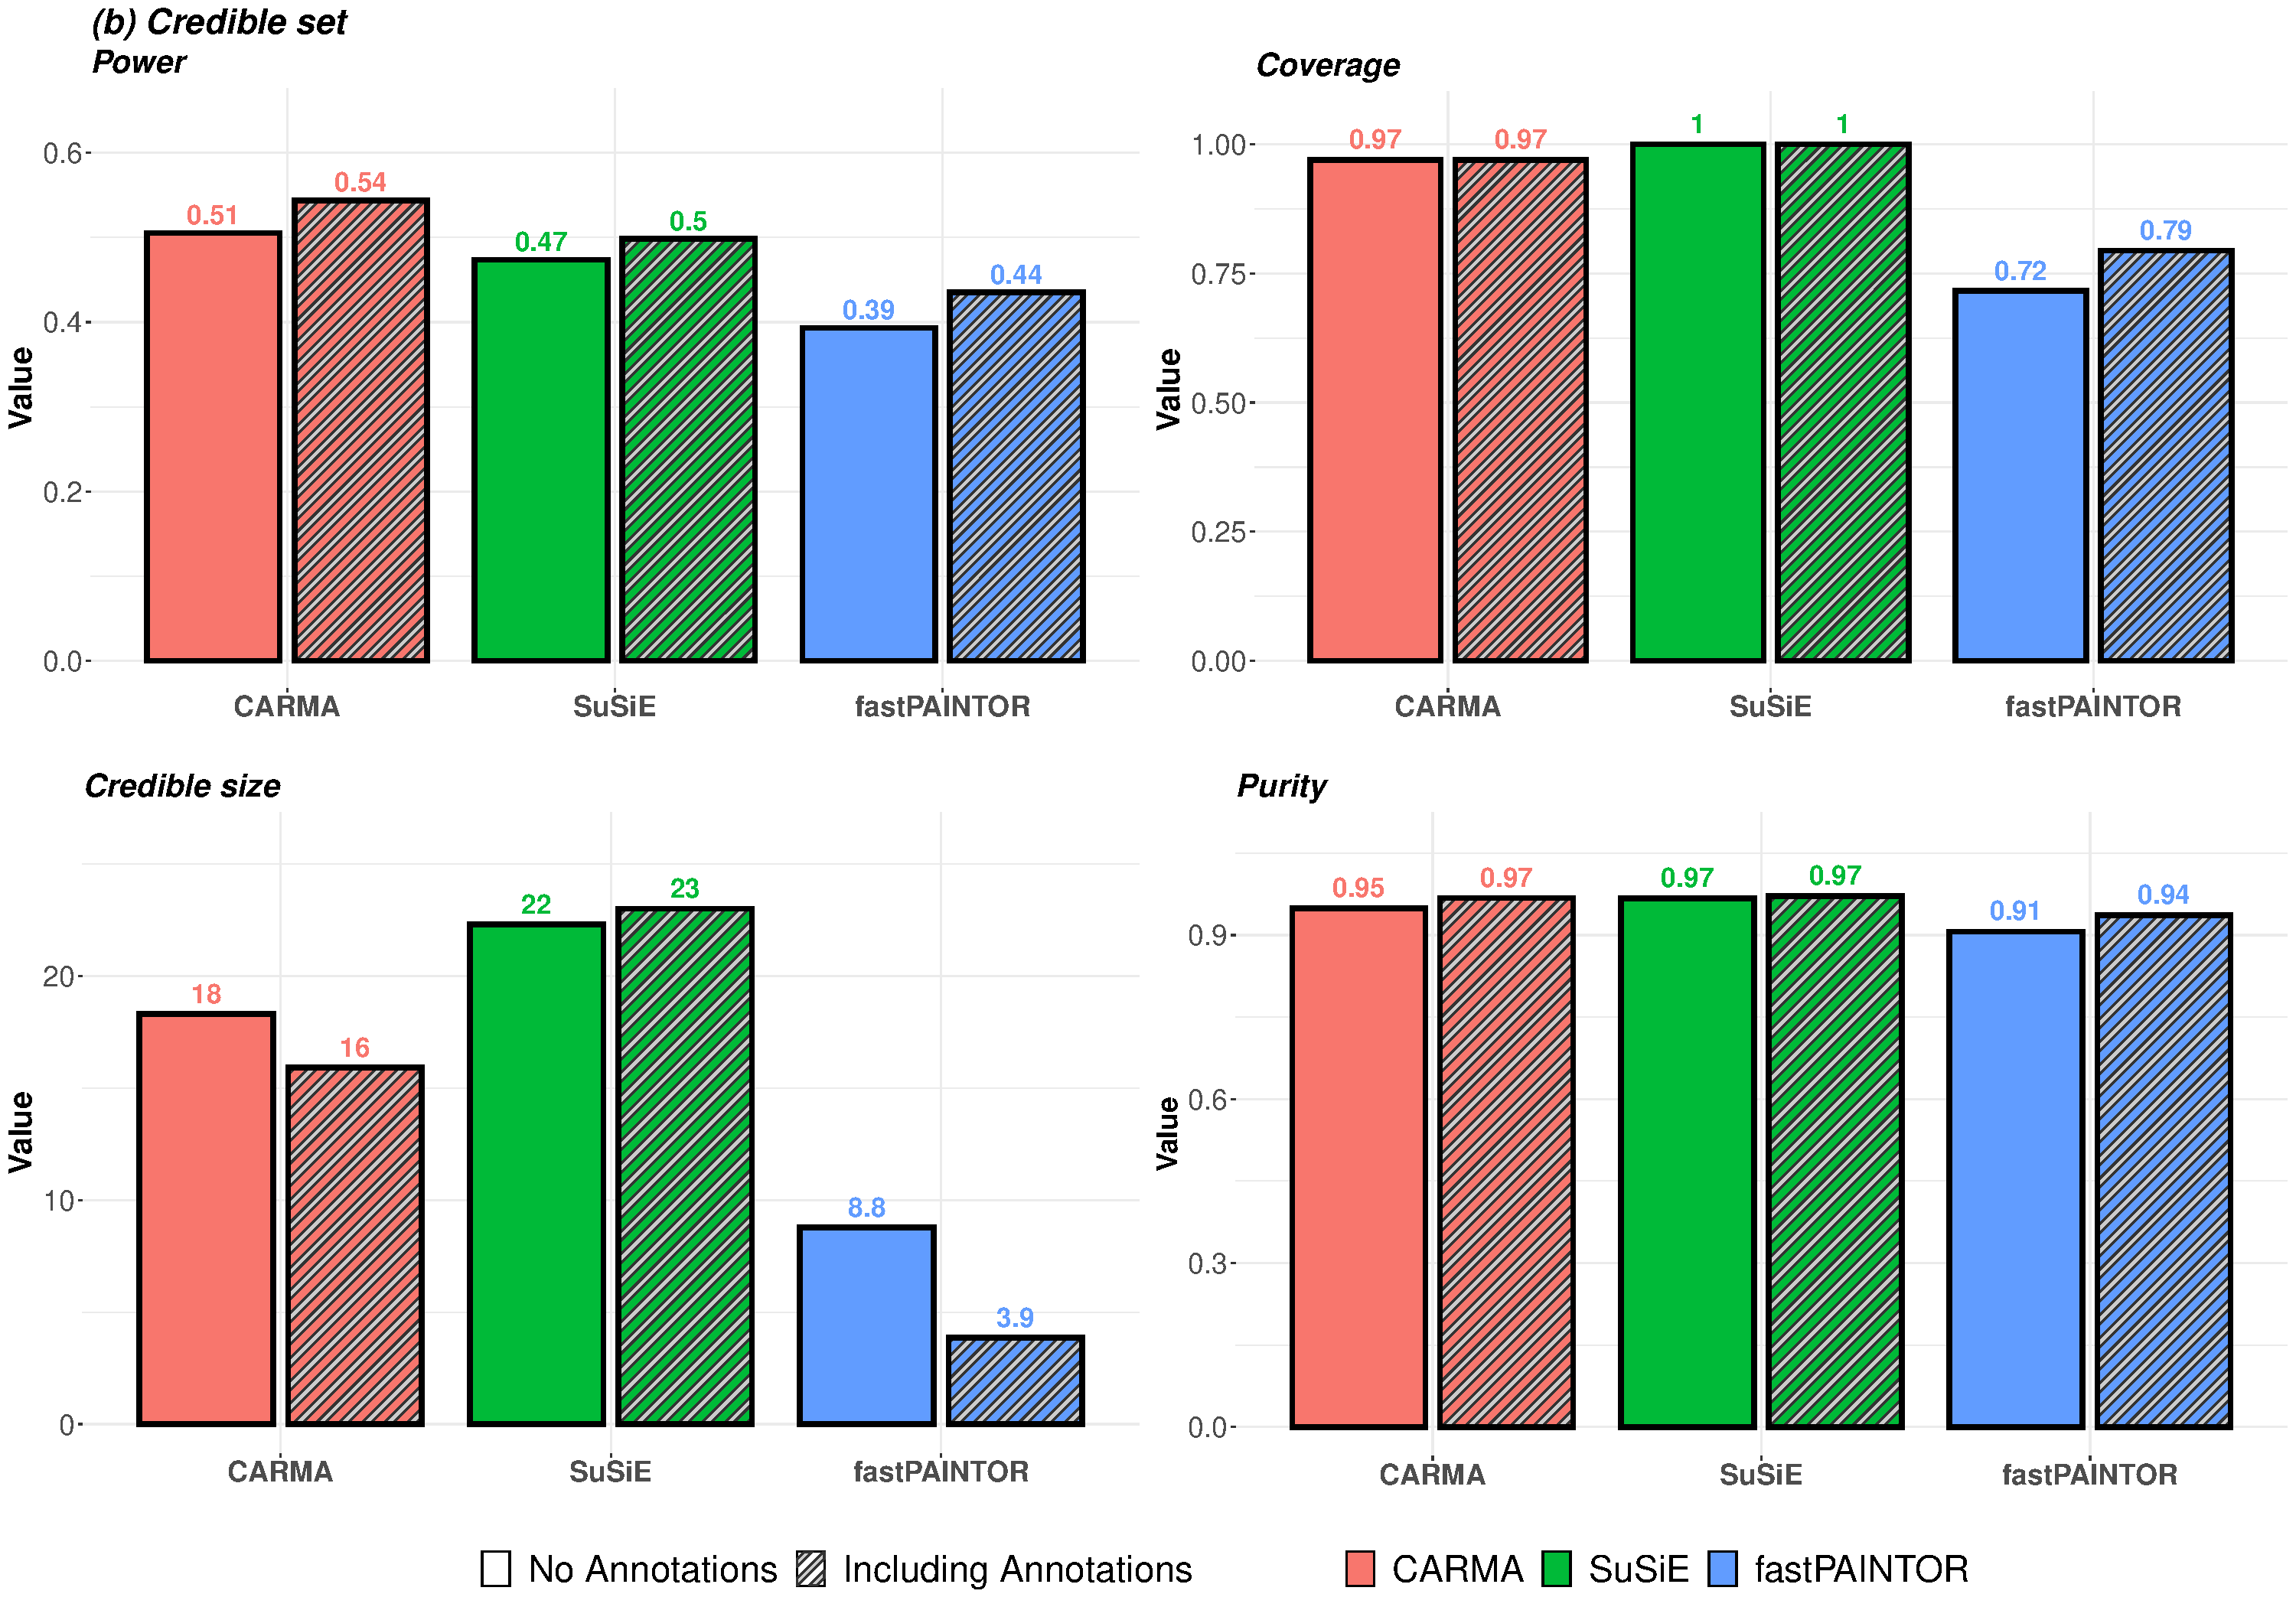
\includegraphics[width=4.3in]{./plots/normal_in-sample_credible_set_|T|=3.pdf} 
   \caption{Performances associated with the credible set. }
   \label{fig:example}
\end{figure}
}
%%%%%%%%%%%%%%%%%%%%%%%%%%%%%%%%%%%%%%%%%%%%%%%%%%%%%%%%%%%%%%%%%%%%%%%%%%%%%%%%%%%%%%
%%%%%%%%%%%%%%%%%%%%%%%%%%%%%%%%%%%%%%%%%%%%%%%%%%%%%%%%%%%%%%%%%%%%%%%%%%%%%%%%%%%%%%
\frame{
\frametitle{Simulation results (no outlier)}
\begin{figure}[htbp] %  figure placement: here, top, bottom, or page
   \centering
   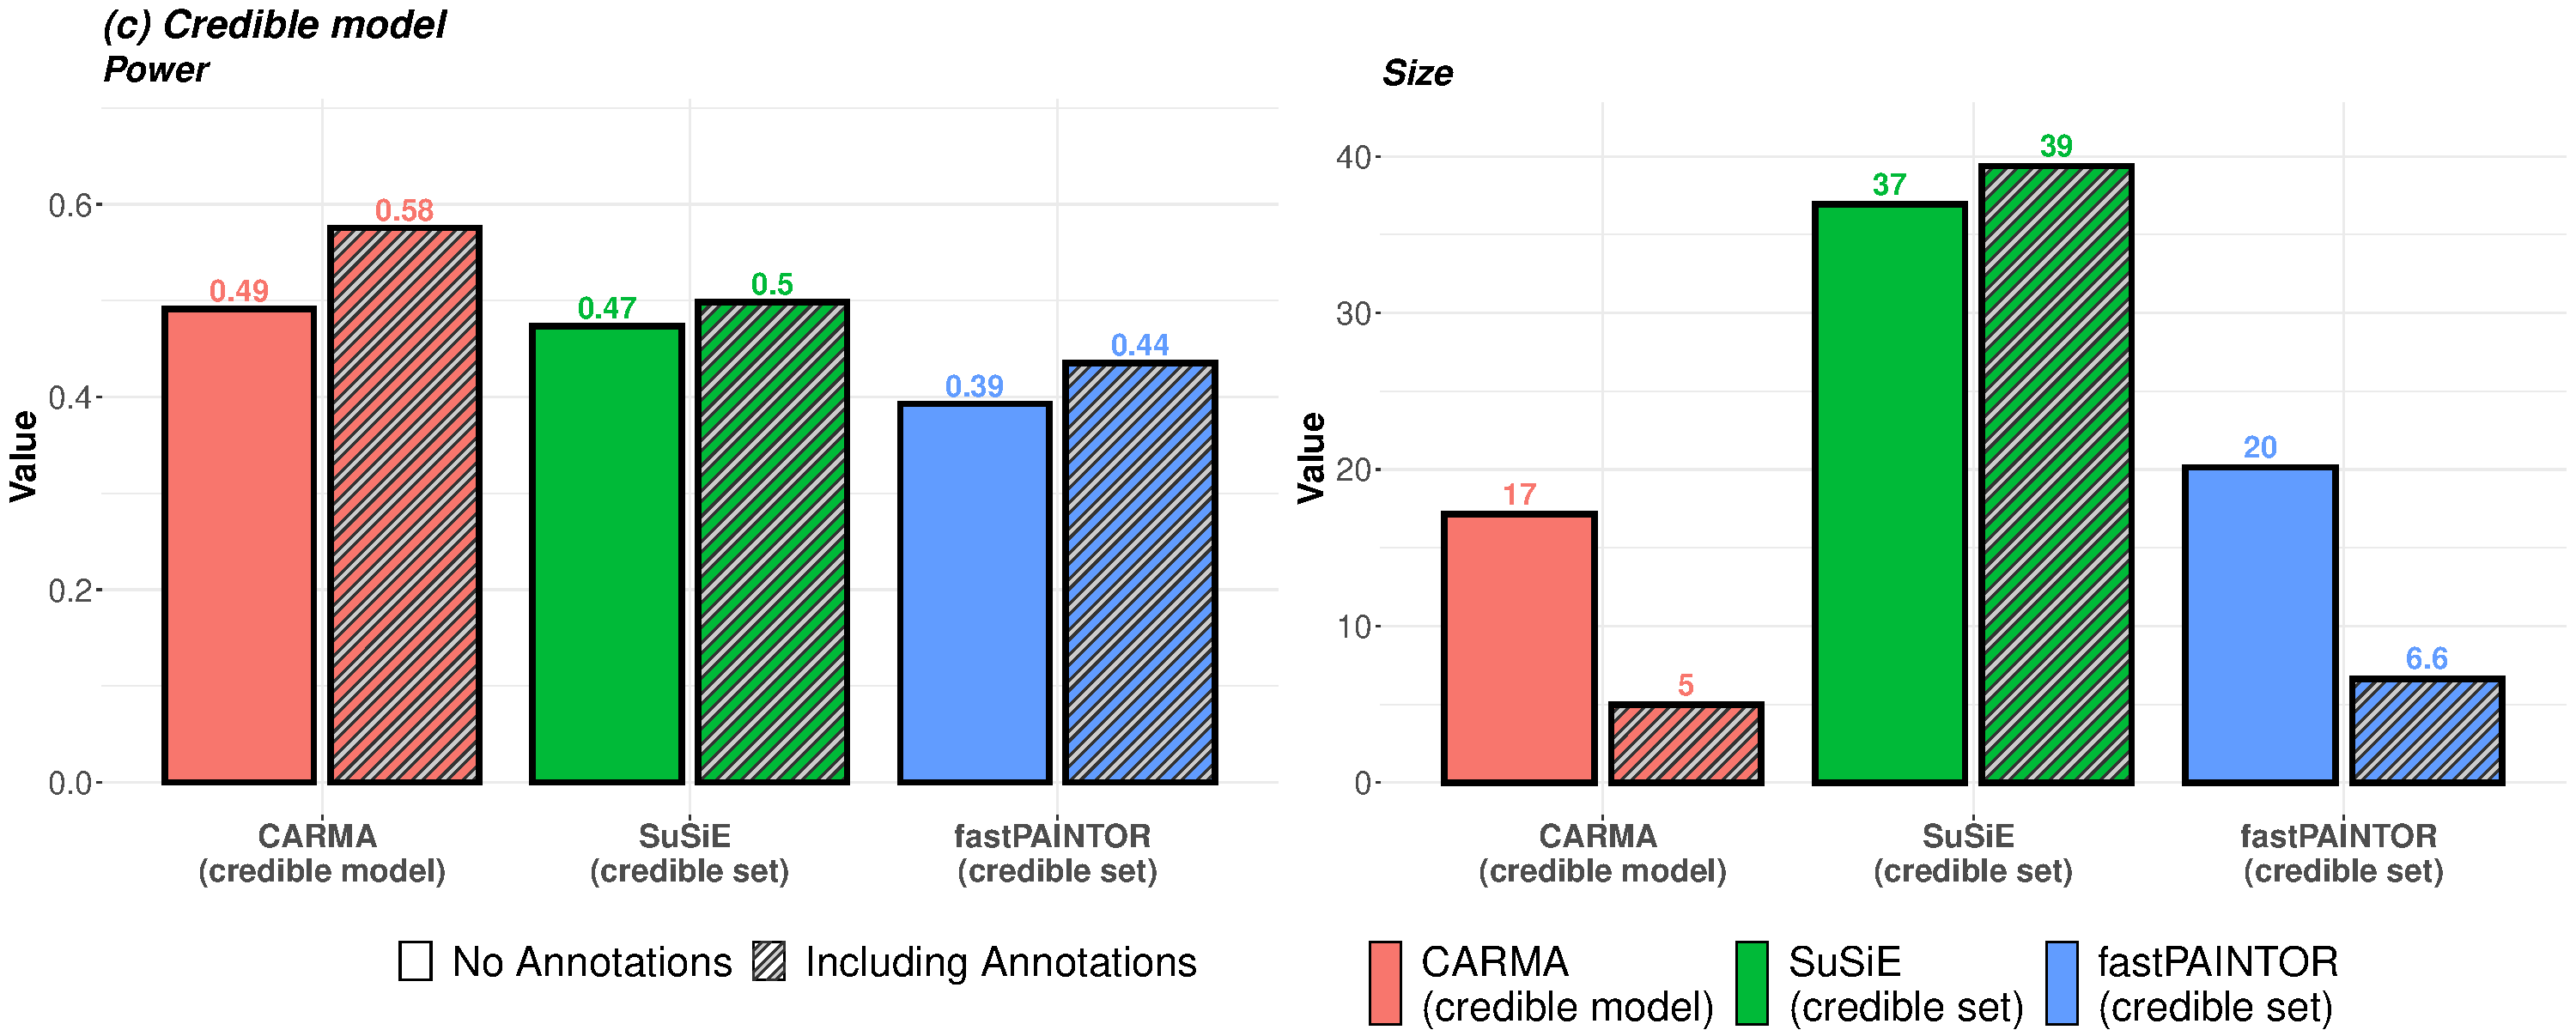
\includegraphics[width=4.5in]{./plots/normal_in-sample_credible_model_|T|=3.pdf} 
   \caption{Credible models and counterparts of SuSiE and fastPAINTOR. }
   \label{fig:example}
\end{figure}
}
%%%%%%%%%%%%%%%%%%%%%%%%%%%%%%%%%%%%%%%%%%%%%%%%%%%%%%%%%%%%%%%%%%%%%%%%%%%%%%%%%%%%%%


%%%%%%%%%%%%%%%%%%%%%%%%%%%%%%%%%%%%%%%%%%%%%%%%%%%%%%%%%%%%%%%%%%%%%%%%%%%%%%%%%%%%%%
\frame{
\frametitle{Simulation results (with outlier)}
\begin{figure}[htbp] %  figure placement: here, top, bottom, or page
   \centering
   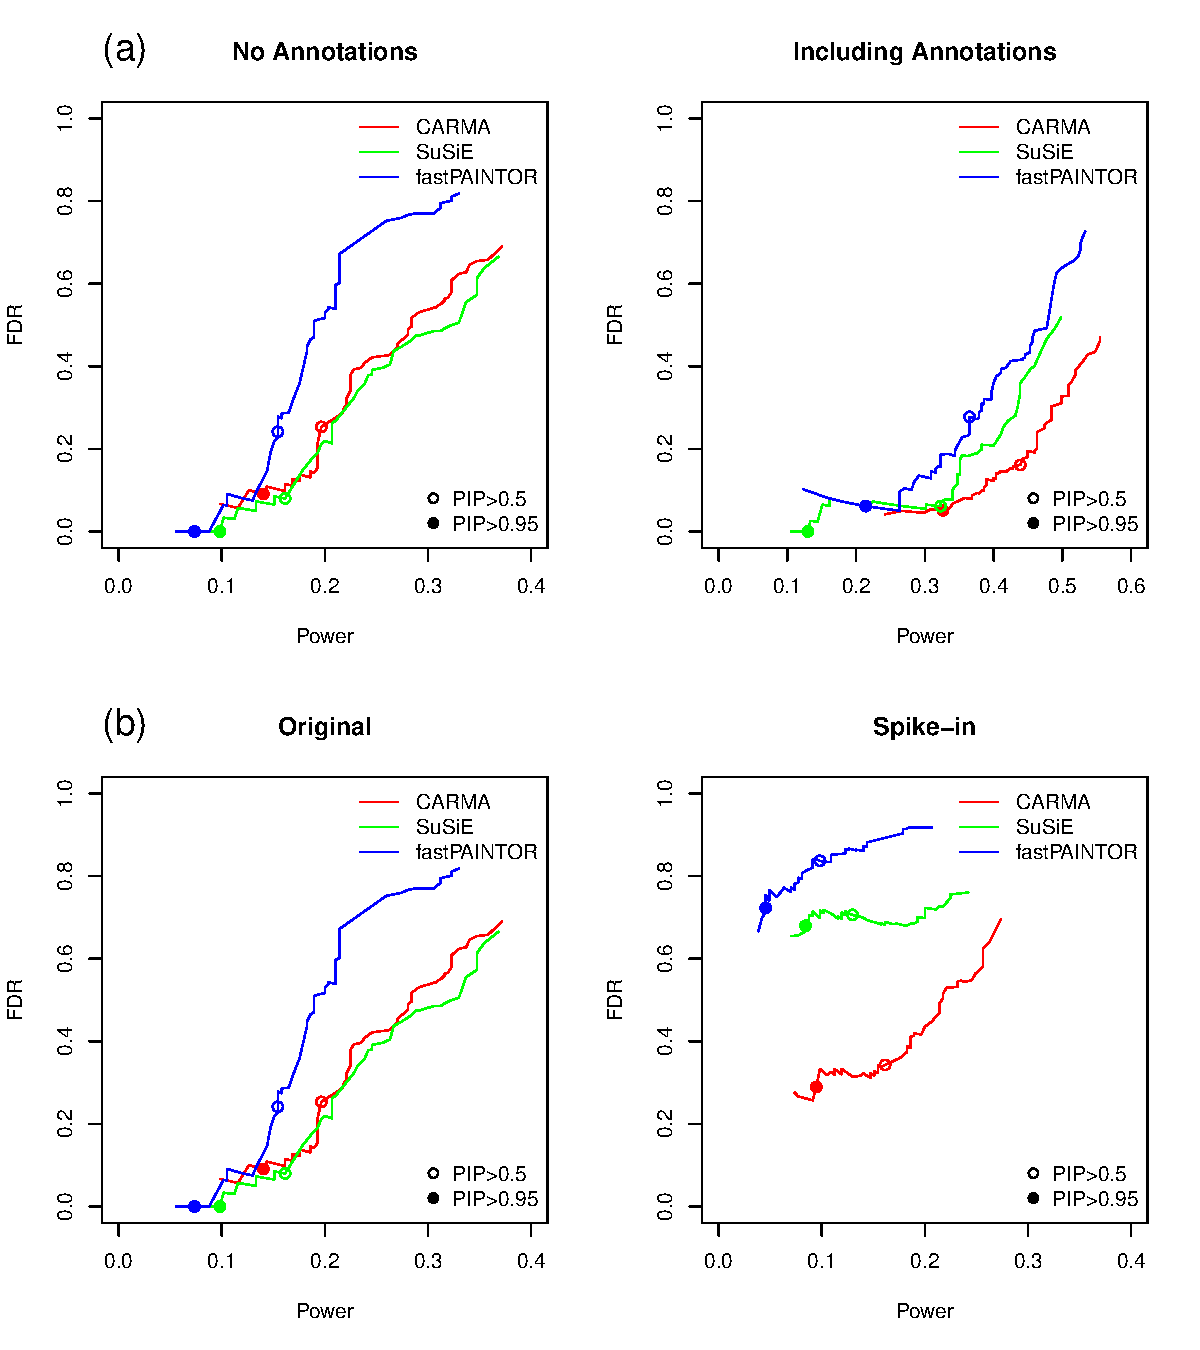
\includegraphics[width=2.8in]{./plots/normal_power_fdr_merged.pdf} 
    %  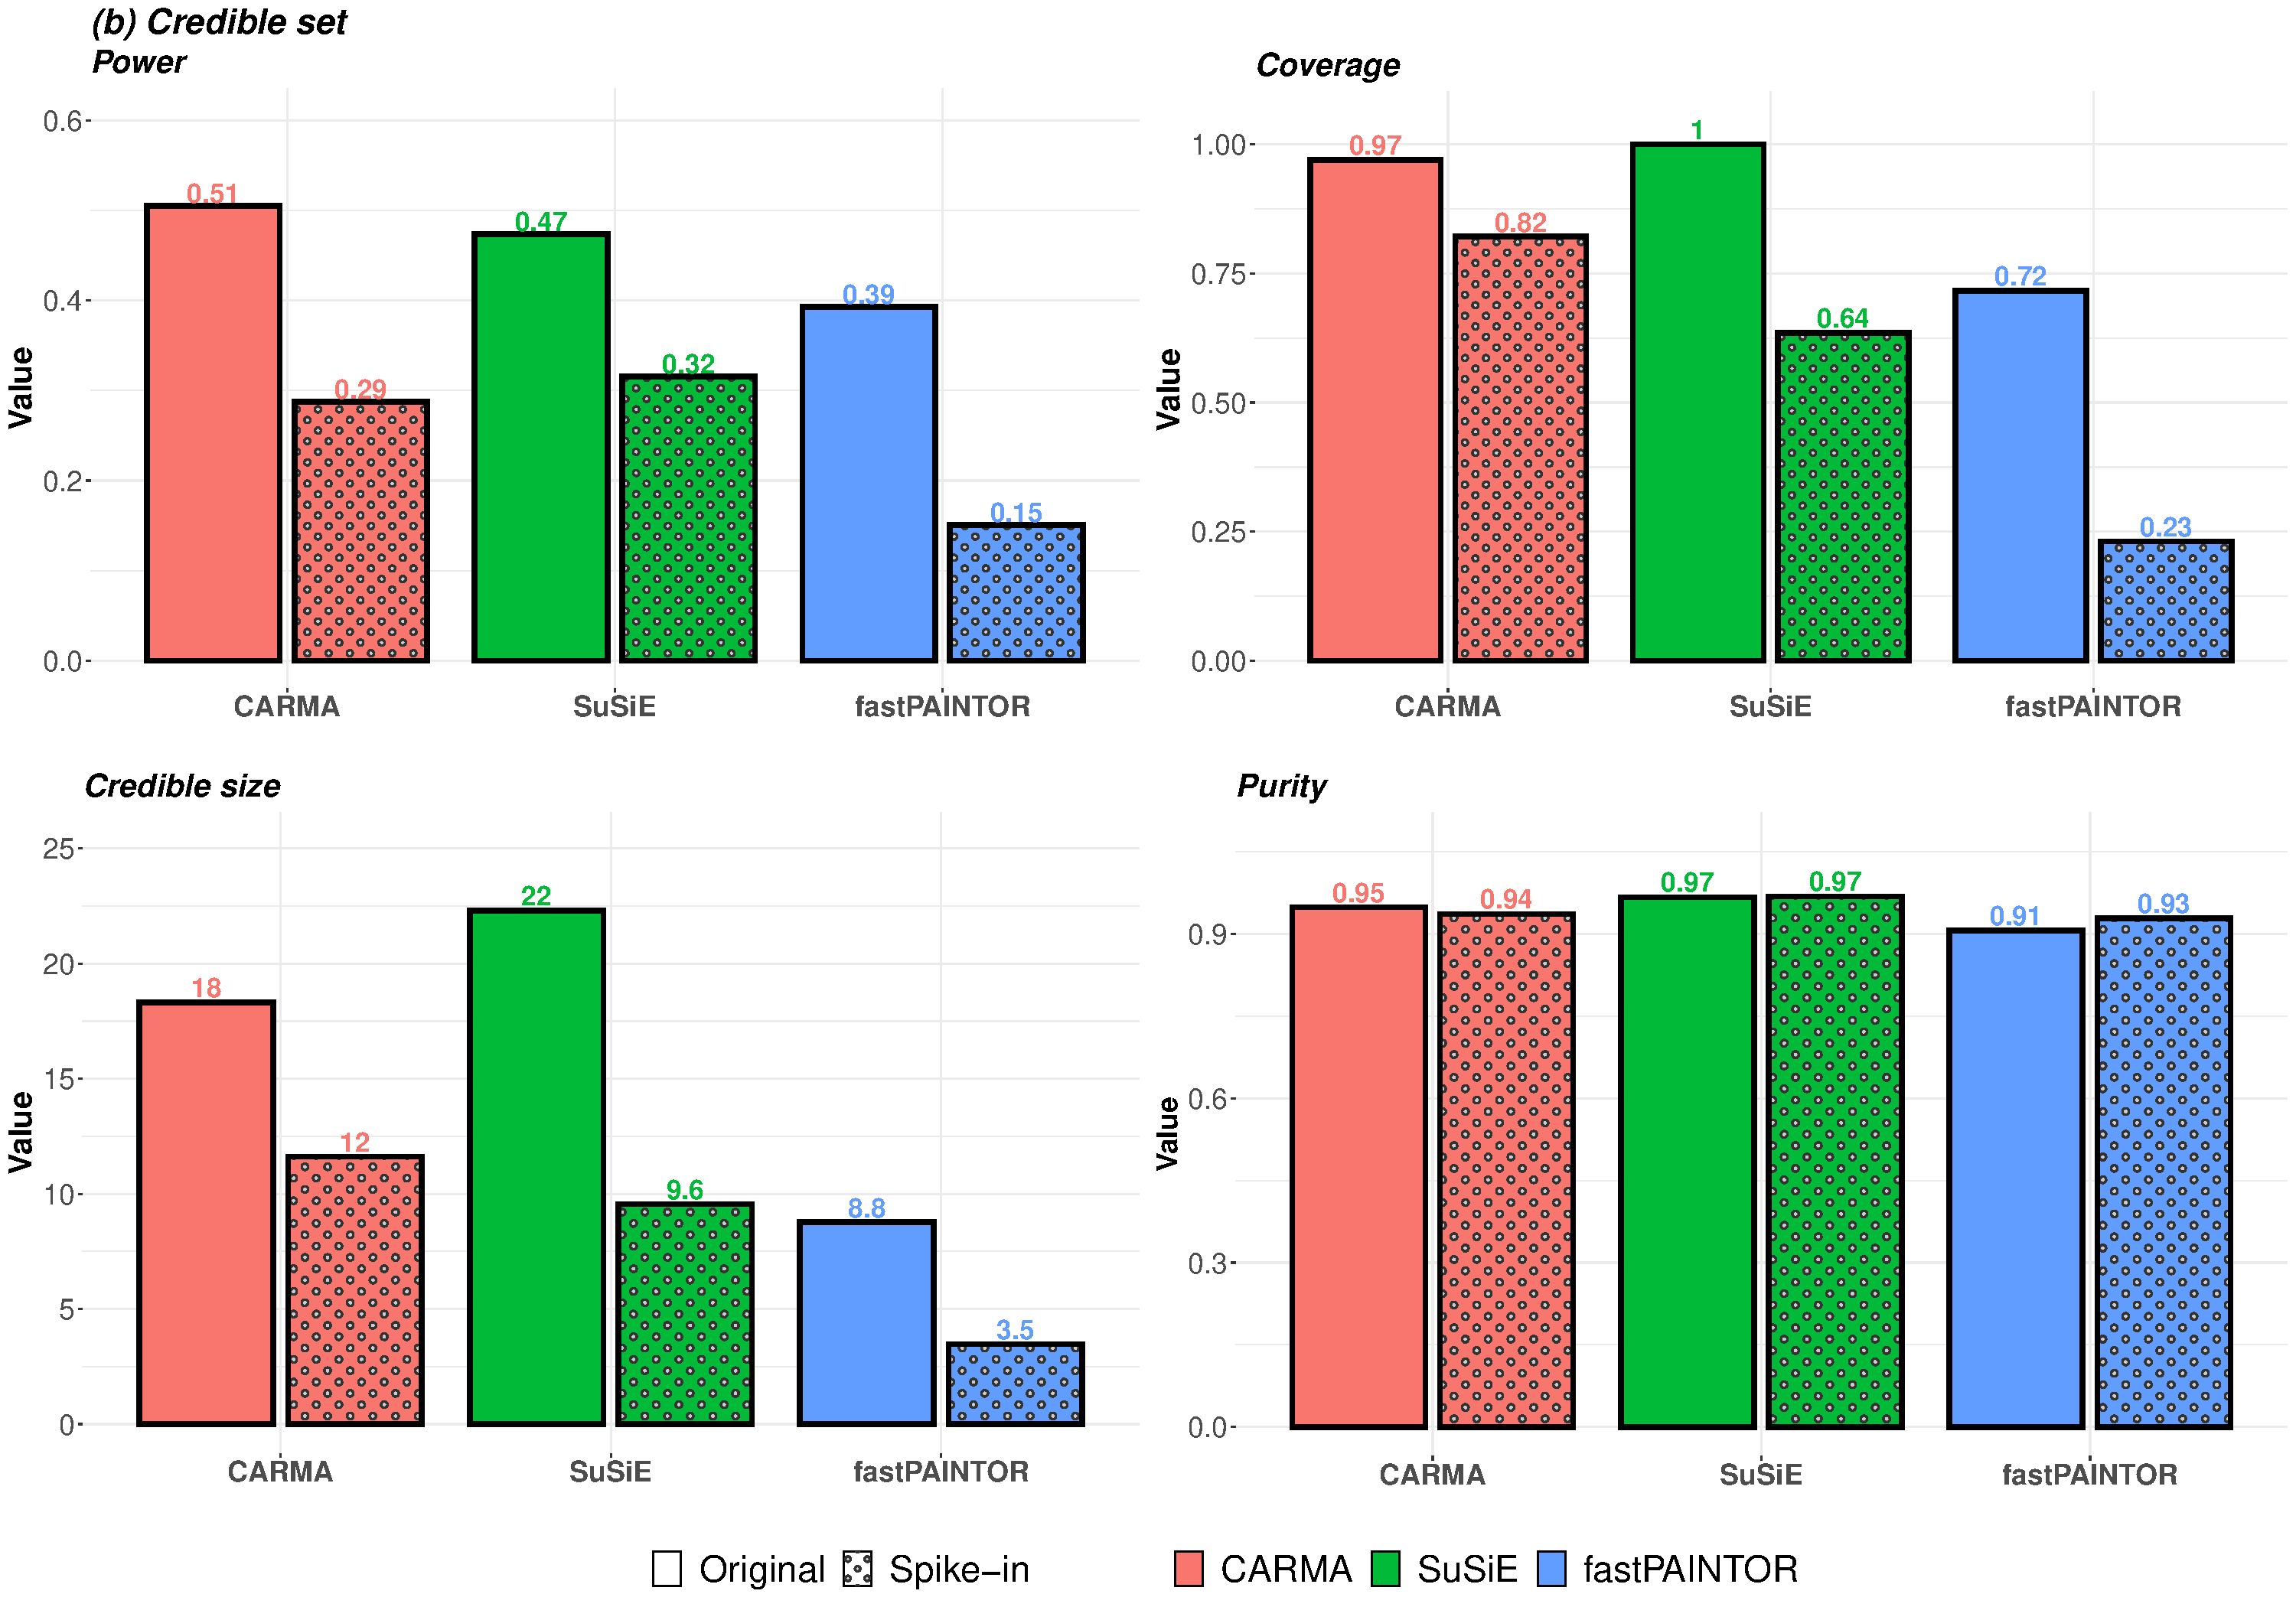
\includegraphics[width=4in]{./plots/normal_outlier_credible_set_|T|=3.pdf} 
 %  \caption{example caption}
   \label{fig:example}
   \end{figure}
}

%%%%%%%%%%%%%%%%%%%%%%%%%%%%%%%%%%%%%%%%%%%%%%%%%%%%%%%%%%%%%%%%%%%%%%%%%%%%%%%%%%%%%%
%%%%%%%%%%%%%%%%%%%%%%%%%%%%%%%%%%%%%%%%%%%%%%%%%%%%%%%%%%%%%%%%%%%%%%%%%%%%%%%%%%%%%%
\frame[t]{
\frametitle{Real data (AD study \cite{jansen2019genome})}
\begin{block}{Data process}
\begin{itemize}
\item We present fine-mapping results  at 30 GWAS loci  identified in a large  meta-analysis of  clinically diagnosed AD and AD-by-proxy with 71,880 cases and 383,378 controls of European ancestry \cite{jansen2019genome}.
\item For the CARMA model, we include 924 functional annotations including  DeepSEA \cite{zhou2015predicting}, CADD \cite{kircher2014general}, PO-EN \cite{yang2021semisupervised}, and PolyFun \cite{weissbrod2020functionally}.
\item For each model, we consider two scenarios: 
\begin{itemize}
\item[1] no functional annotation
\item[2] including functional annotations
\end{itemize}
\end{itemize}
\end{block}
\begin{block}{Challenges}
\begin{itemize}
\item  The sample sizes can vary from 9,703 to 444,006 depending on which datasets are included in the meta-analyses.
\item The LD matrix is extracted from AD-by-proxy dataset (UK Biobank). 
\item Severe discrepancies between Z/LD.
\end{itemize}
\end{block}
}
%%%%%%%%%%%%%%%%%%%%%%%%%%%%%%%%%%%%%%%%%%%%%%%%%%%%%%%%%%%%%%%%%%%%%%%%%%%%%%%%%%%%%%

%%%%%%%%%%%%%%%%%%%%%%%%%%%%%%%%%%%%%%%%%%%%%%%%%%%%%%%%%%%%%%%%%%%%%%%%%%%%%%%%%%%%%%
\frame[t]{
\frametitle{Real data (AD study \cite{jansen2019genome})}
\begin{figure}[htbp] %  figure placement: here, top, bottom, or page
   \centering
   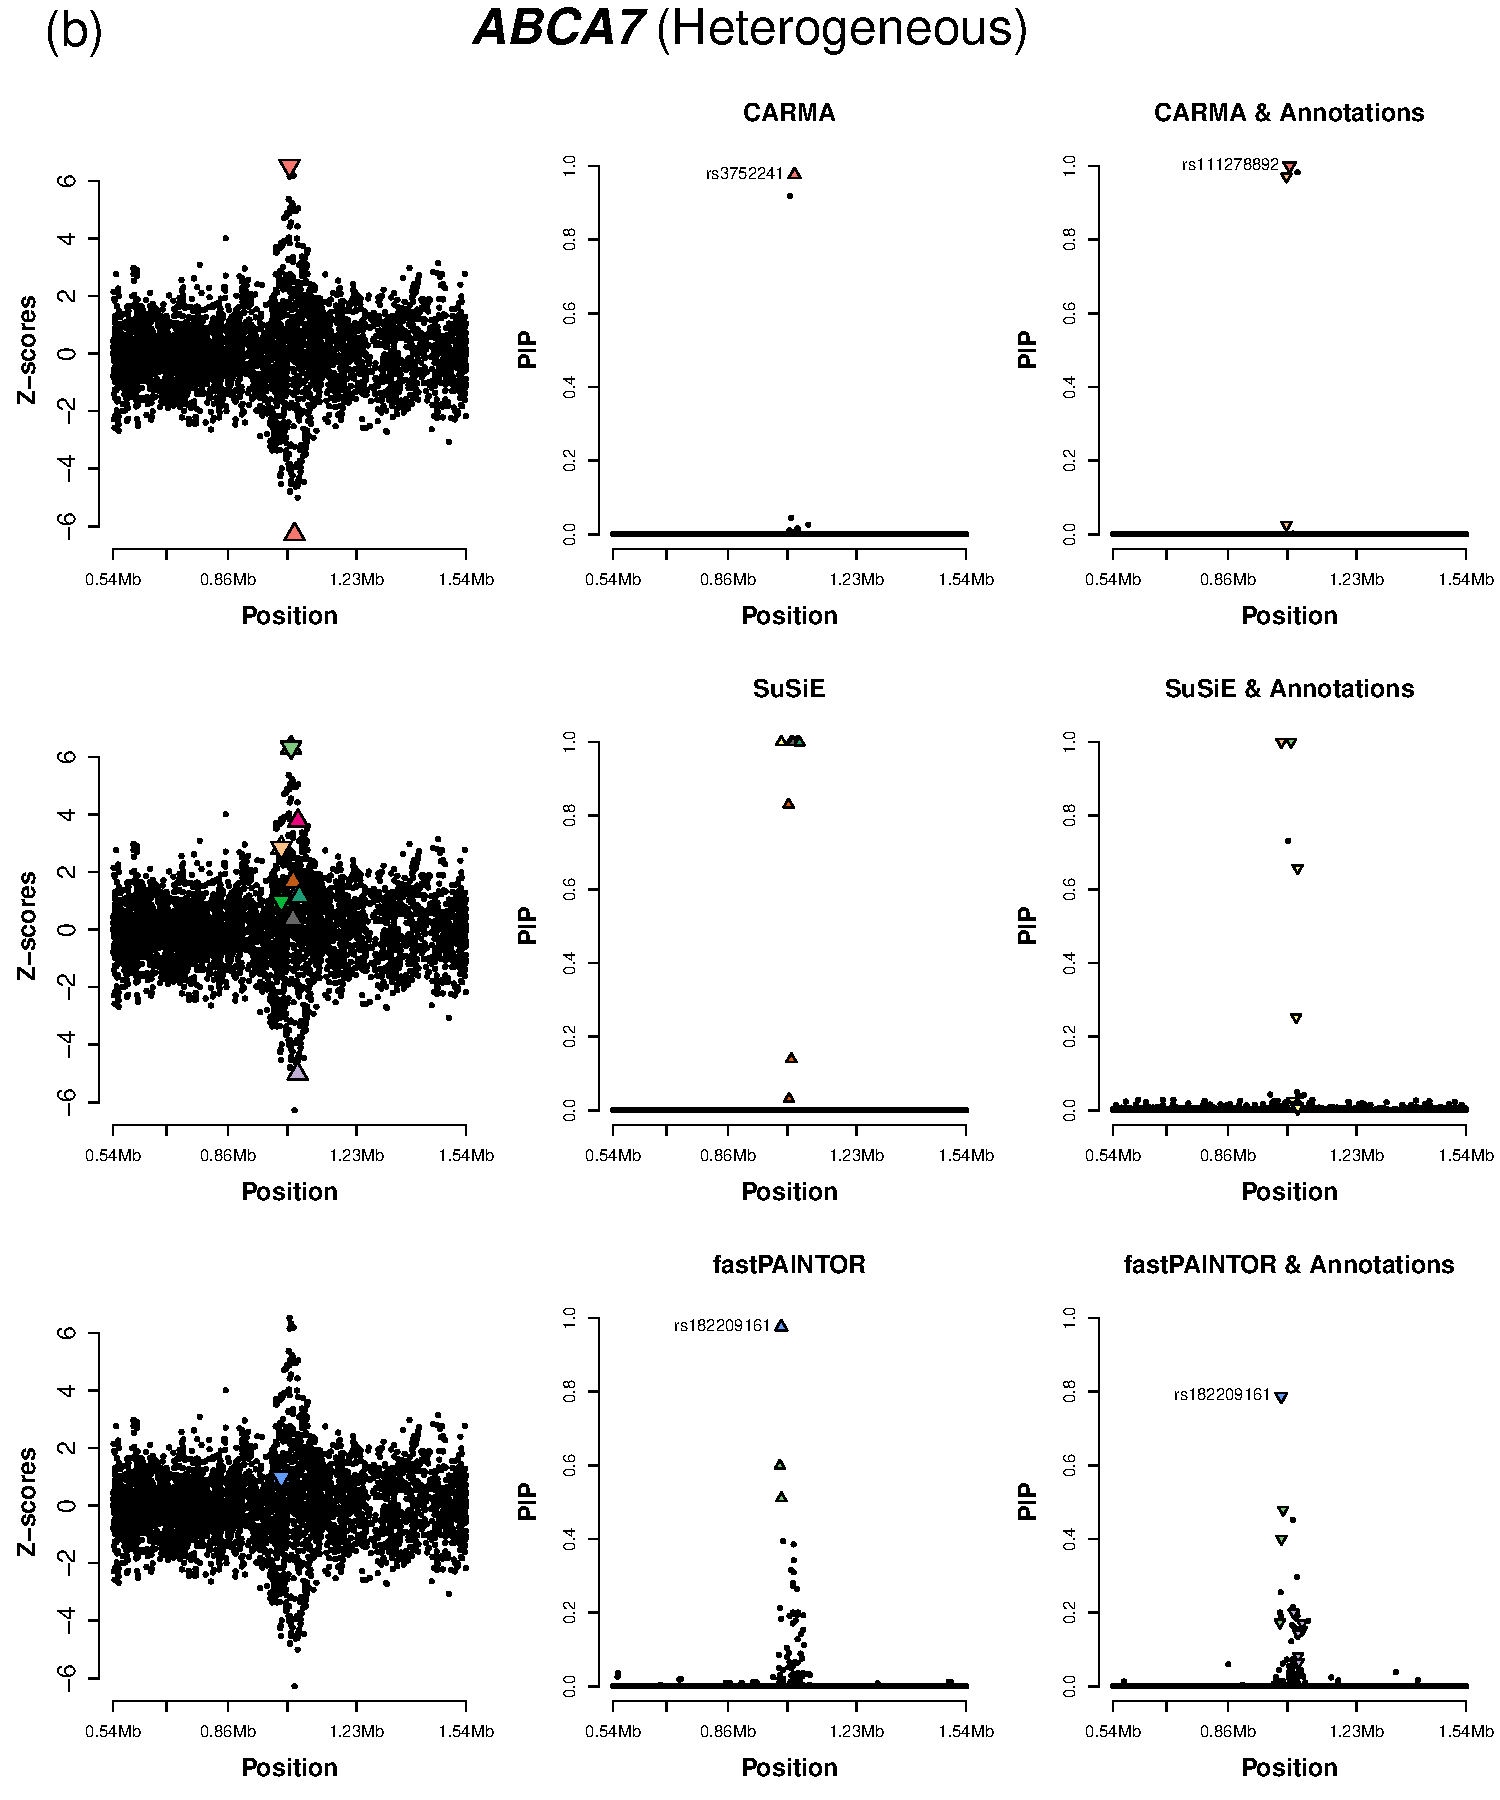
\includegraphics[width=2.5in]{./plots/ABCA7.pdf} 
   \caption{ Locus{\it ABCA7}. }
   \label{fig:example}
\end{figure}
}
%%%%%%%%%%%%%%%%%%%%%%%%%%%%%%%%%%%%%%%%%%%%%%%%%%%%%%%%%%%%%%%%%%%%%%%%%%%%%%%%%%%%%%
%%%%%%%%%%%%%%%%%%%%%%%%%%%%%%%%%%%%%%%%%%%%%%%%%%%%%%%%%%%%%%%%%%%%%%%%%%%%%%%%%%%%%%
\frame[t]{
\frametitle{Real data (AD study \cite{jansen2019genome})}
\begin{figure}[htbp] %  figure placement: here, top, bottom, or page
   \centering
   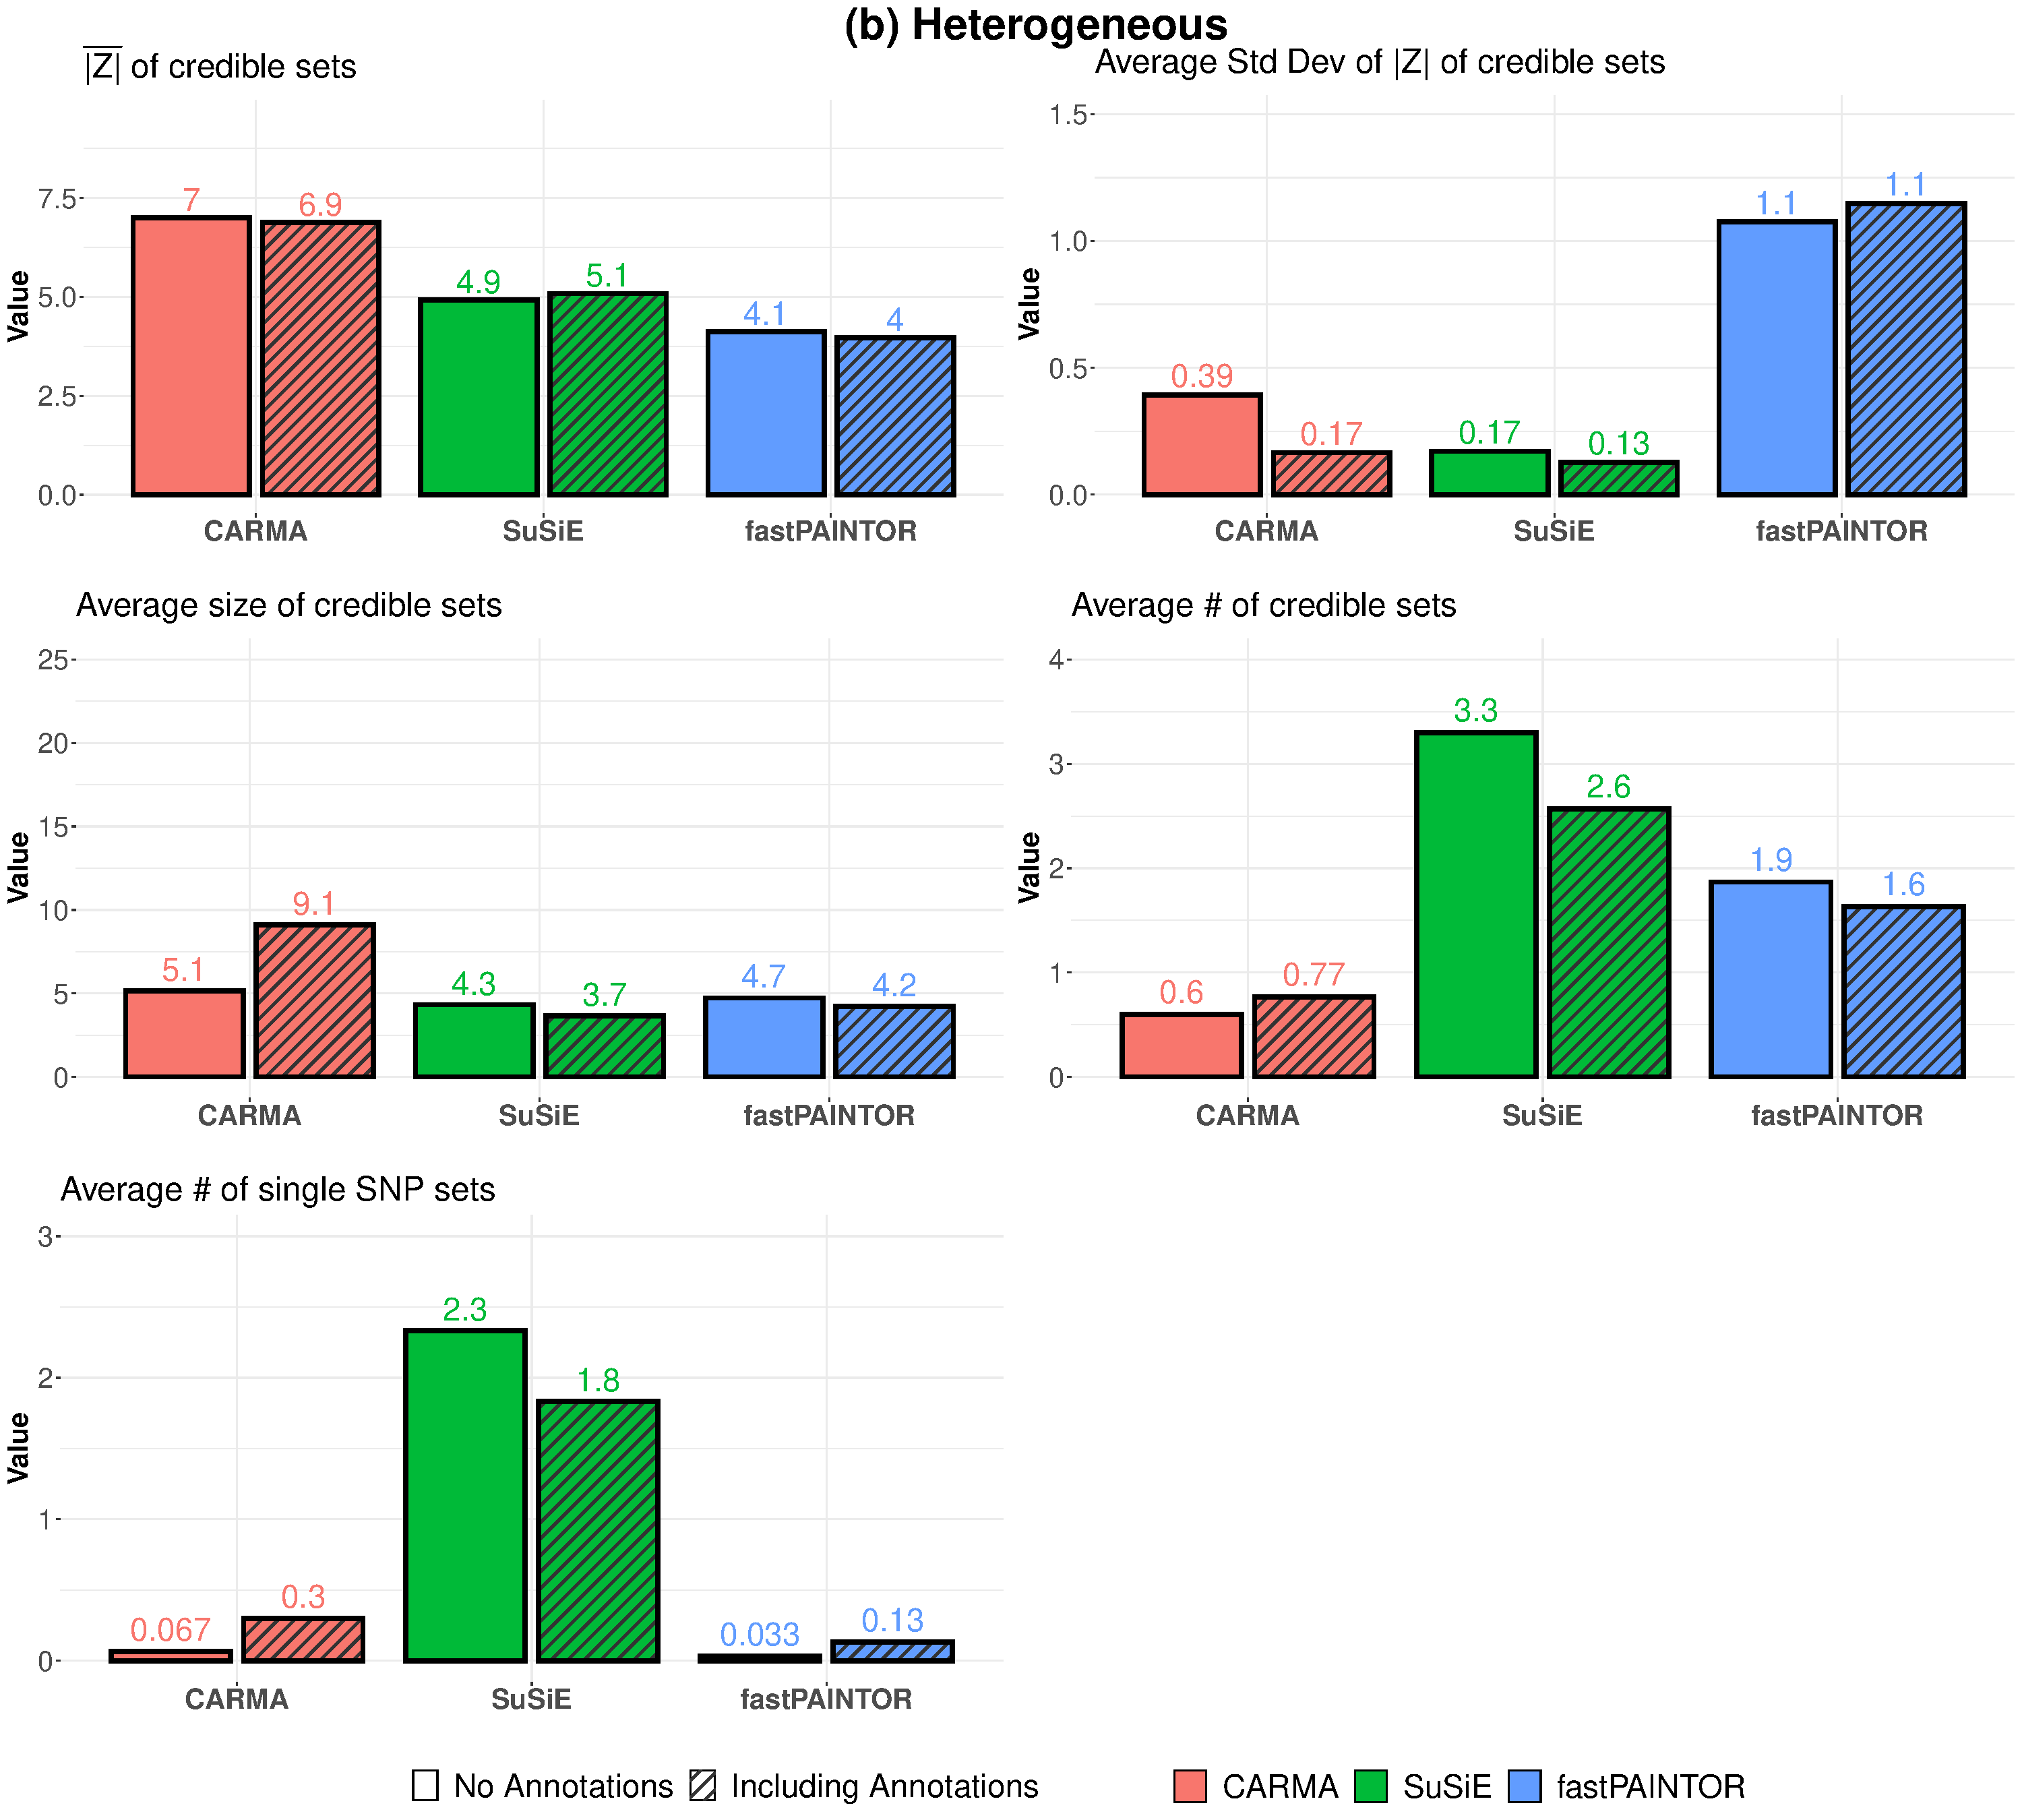
\includegraphics[width=3in]{./plots/AD_credible_set_099_hetero_adaptive_by_model_separated.pdf} 
   \caption{Summary of the all 30 loci.  }
   \label{fig:example}
\end{figure}
}
%%%%%%%%%%%%%%%%%%%%%%%%%%%%%%%%%%%%%%%%%%%%%%%%%%%%%%%%%%%%%%%%%%%%%%%%%%%%%%%%%%%%%%

%%%%%%%%%%%%%%%%%%%%%%%%%%%%%%%%%%%%%%%%%%%%%%%%%%%%%%%%%%%%%%%%%%%%%%%%%%%%%%%%%%%%%%

%%%%%%%%%%%%%%%%%%%%%%%%%%%%%%%%%%%%%%%%%%%%%%%%%%%%%%%%%%%%%%%%%%%%%%%%%%%%%%%%%%%%%%
%%%%%%%%%%%%%%%%%%%%%%%%%%%%%%%%%%%%%%%%%%%%%%%%%%%%%%%%%%%%%%%%%%%%%%%%%%%%%%%%%%%%%%
\frame{
\frametitle{Future researches}
\begin{block}{CARMA}
\begin{itemize}
\item The paper has been submitted to NATURE Genetics, under review now. 
\item The R package is on GitHub with user manual. 
\item The authors are Zikun Yang, Chen Wang, Atlas Khan, Badri Vardarajan, Richard Mayeux, Krzysztof Kiryluk, Iuliana Ionita-Laza.
\end{itemize}
\end{block}

\begin{block}{Statistical genetics}
\begin{itemize}
\item Currently, I am working on a better solution of the outlier detection with extra information of the meta-analysis. 
\item Working on developing multi-ethnics fine-mapping method, i.e. combining European, African, East Asian, etc.. Considering structure of variational Bayes that I am totally not familiar with :). 
\item Working on a real data of Alzheimer's disease based on the subjects from Dominican, Mexican, Peru, and ethnics associated with Caribbean are. Largest datasets of such cohorts to date. 
\end{itemize}
\end{block}
\begin{block}{Bayesian Statistic}
\begin{itemize}
\item Working on the Heavy-tailed Horseshoe prior, finishing paper. 
\item Trying to replace LMM model in genetics with Horseshoe prior. 
\end{itemize}
\end{block}
}

%%%%%%%%%%%%%%%%%%%%%%%%%%%%%%%%%%%%%%%%%%%%%%%%%%%%%%%%%%%%%%%%%%%%%%%%%%%%%%%%%%%%%%
\frame{
\frametitle{Special thank}
\begin{block}{Special thanks to}
\begin{itemize}
\item Dr. Ionita-Laza 
\item Dr. Womack 
\end{itemize}
\end{block}
}

%%%%%%%%%%%%%%%%%%%%%%%%%%%%%%%%%%%%%%%%%%%%%%%%%%%%%%%%%%%%%%%%%%%%%%%%%%%%%%%%%%%%%%
%%%%%%%%%%%%%%%%%%%%%%%%%%%%%%%%%%%%%%%%%%%%%%%%%%%%%%%%%%%%%%%%%%%%%%%%%%%%%%%%%%%%%%
\frame{
\frametitle{Thank you all!}
\center
\Huge
THANK YOU!
}

\frame{
\bibliography{UNL_talk.bib}
\bibliographystyle{apalike}
}

%%%%%%%%%%%%%%%%%%%%%%%%%%%%%%%%%%%%%%%%%%%%%%%%%%%%%%%%%%%%%%%%%%%%%%%%%%%%%%%%%%%%%%
%%%%%%%%%%%%%%%%%%%%%%%%%%%%%%%%%%%%%%%%%%%%%%%%%%%%%%%%%%%%%%%%%%%%%%%%%%%%%%%%%%%%%%
\frame[t]{
\frametitle{EM-algorithm}
\begin{block}{\small Details of EM-algorithm}
\begin{itemize}
\item Suppose that the truncated model space $\Gamma$ of the top $B$ models with the largest posterior probabilities. 
\item Let $\boldsymbol G'=\lrc{G_1,\ldots,G_p}$ denote the count vector associated with $\Gamma$, where $G_i\in\lrc{0,1,\ldots,B}$ is the count of $\gamma_i=1$ appearing in $\Gamma$. 
\item $\boldsymbol G$ is the missing value. In EM algorithm, we use Poisson regression to model it. 
\item Let $g_i^{\lrp{s}}$ denote the actual count of $\gamma_i$ appearing in $\Gamma^{(s)}$ after running Shotgun algorithm at step $(s)$ of the EM algorithm. 
\item We approximate   $\mathbf{E}\lrb{G_i|\boldsymbol Z,\boldsymbol w_i,\boldsymbol \theta^{(s)}}$ by $g_i^{(s)}$ in EM algorithm.
\end{itemize}
\end{block}
}

\frame[t]{
\frametitle{EM-algorithm}
\fontsize{7pt}{7pt}
 \begin{algorithm}[H]
\footnotesize
 Input: Summary statistics $\boldsymbol Z$, functional annotations $W$, hyperparameter $\eta$ of the Poisson prior distribution, and $B$. \\
Initialization: Run Shotgun algorithm with the prior distribution Poisson$(\eta)$ to generate $\Gamma^{(0)}$ and $\boldsymbol g^{(0)}$. \\
 \For{$s=0,1,\ldots$}{
\begin{itemize}
\item[-] \textbf{EM}\\
 \begin{itemize}
   \item[\textbf{E-step}] Replace $G_i$  by $\mathbf{E}\lrb{G_i|\boldsymbol Z,\boldsymbol w_i,\boldsymbol \theta^{(s)}}$, which is approximated by $g^{(s)}_i$,  $i=1,\ldots,p$.   
   \item[\textbf{M-step}] Maximize the penalized log-likelihood as,   \[
    \boldsymbol \theta^{(s+1)}:= \stackrel[\boldsymbol \theta\in R^{q+1}]{}{\text{argmax}} \sum_{i=1}^p\lrb{g^{(s)}_i\boldsymbol w_i'\boldsymbol \theta-\exp{\boldsymbol w_i'\boldsymbol \theta}}-\frac{(1-\alpha)}{2}||\boldsymbol\theta||^2-\alpha||\boldsymbol \theta||.
  \] 
  \end{itemize}
Adjust the prior probability to introduce the multiplicity control (see details below),
      \begin{align}
   \hat{\theta}_1^{(s+1)}&=\log{\frac{\eta B^{(s)}}{\eta+p}}.
   \end{align}
 Then, compute the prior probability of the $(s+1)$ step:
    \begin{align}
  \hat{\text{Pr}}\lrp{\gamma_i=1|\boldsymbol w_i,\boldsymbol \theta^{(s+1)}}=\frac{\exp{\boldsymbol w_i'\boldsymbol \theta^{(s+1)}}}{B^{(s)}}\label{eq::prior_prob_func},
  \end{align} 
 where $B^{(s)}$ is the minimum between $B$ and the total number of models visited by the Shotgun algorithm in step $(s)$.
\item[-] \textbf{Shotgun}\\
Initiate Shotgun algorithm with the estimated prior probability vector $\lrc{  \hat{\text{Pr}}(\gamma_1),\ldots,  \hat{\text{Pr}}(\gamma_p)}'$. After running Shotgun algorithm, acquire $\Gamma^{(s+1)}$ and $\boldsymbol g^{(s+1)}$, which depends on $\boldsymbol Z$, $W$, and $\boldsymbol \theta^{(s+1)}$.  
\end{itemize}
 }
\setcounter{algocf}{0}
  \caption{EM algorithm with functional annotations. }
        \label{al::cps} 
\end{algorithm}~\\


}
%%%%%%%%%%%%%%%%%%%%%%%%%%%%%%%%%%%%%%%%%%%%%%%%%%%%%%%%%%%%%%%%%%%%%%%%%%%%%%%%%%%%%%
\frame{
\frametitle{Simulation results (with outlier)}
\begin{columns}[T]
\begin{column}{0.48\textwidth}
\begin{figure}[htbp] %  figure placement: here, top, bottom, or page
   \centering
   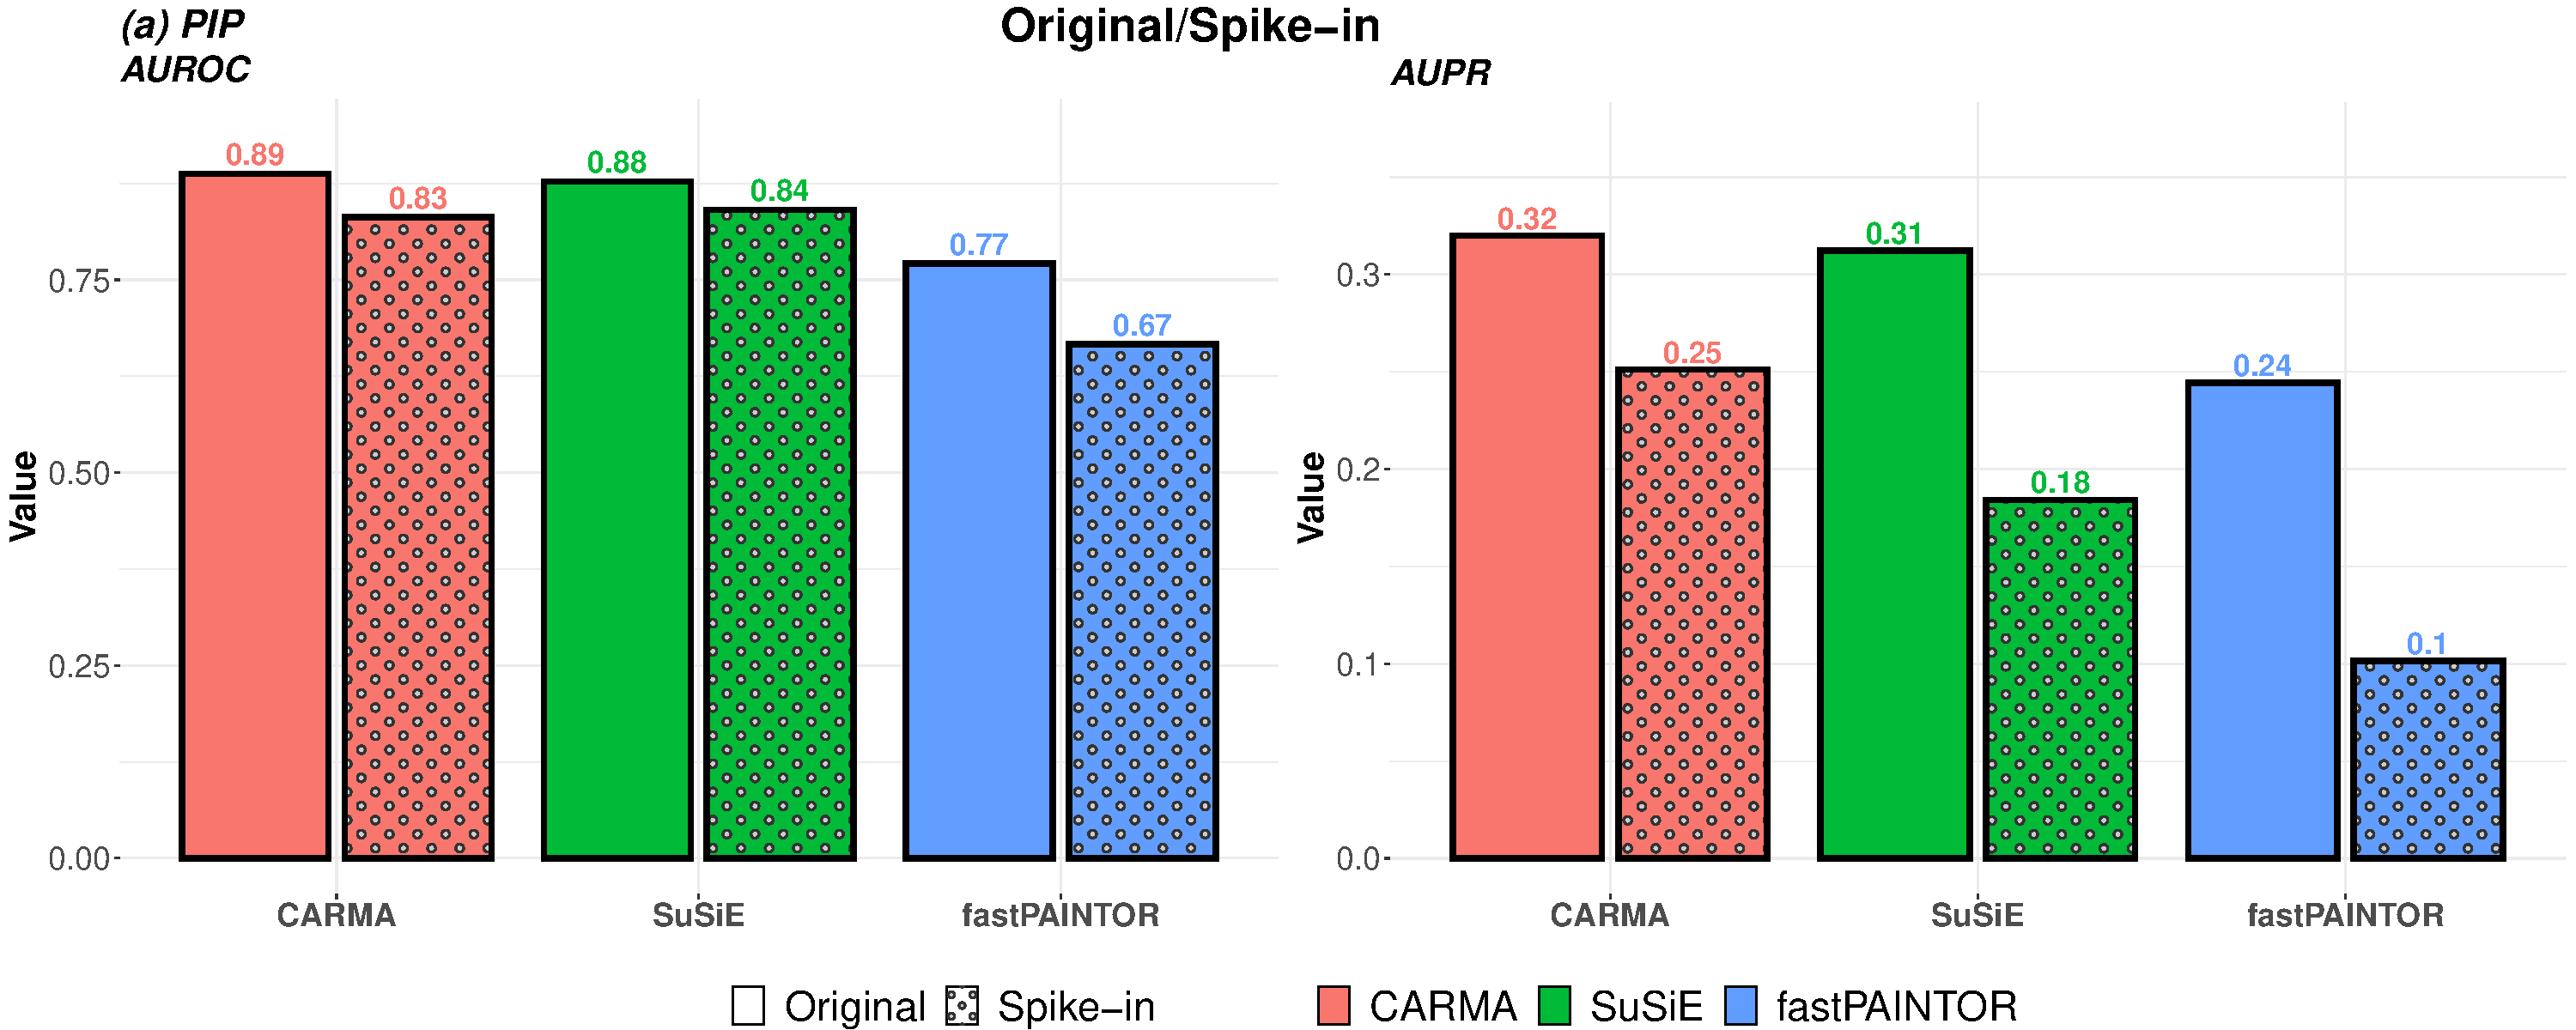
\includegraphics[width=2.5in]{./plots/normal_outlier_AUPR_AUROC_|T|=3.pdf} 
      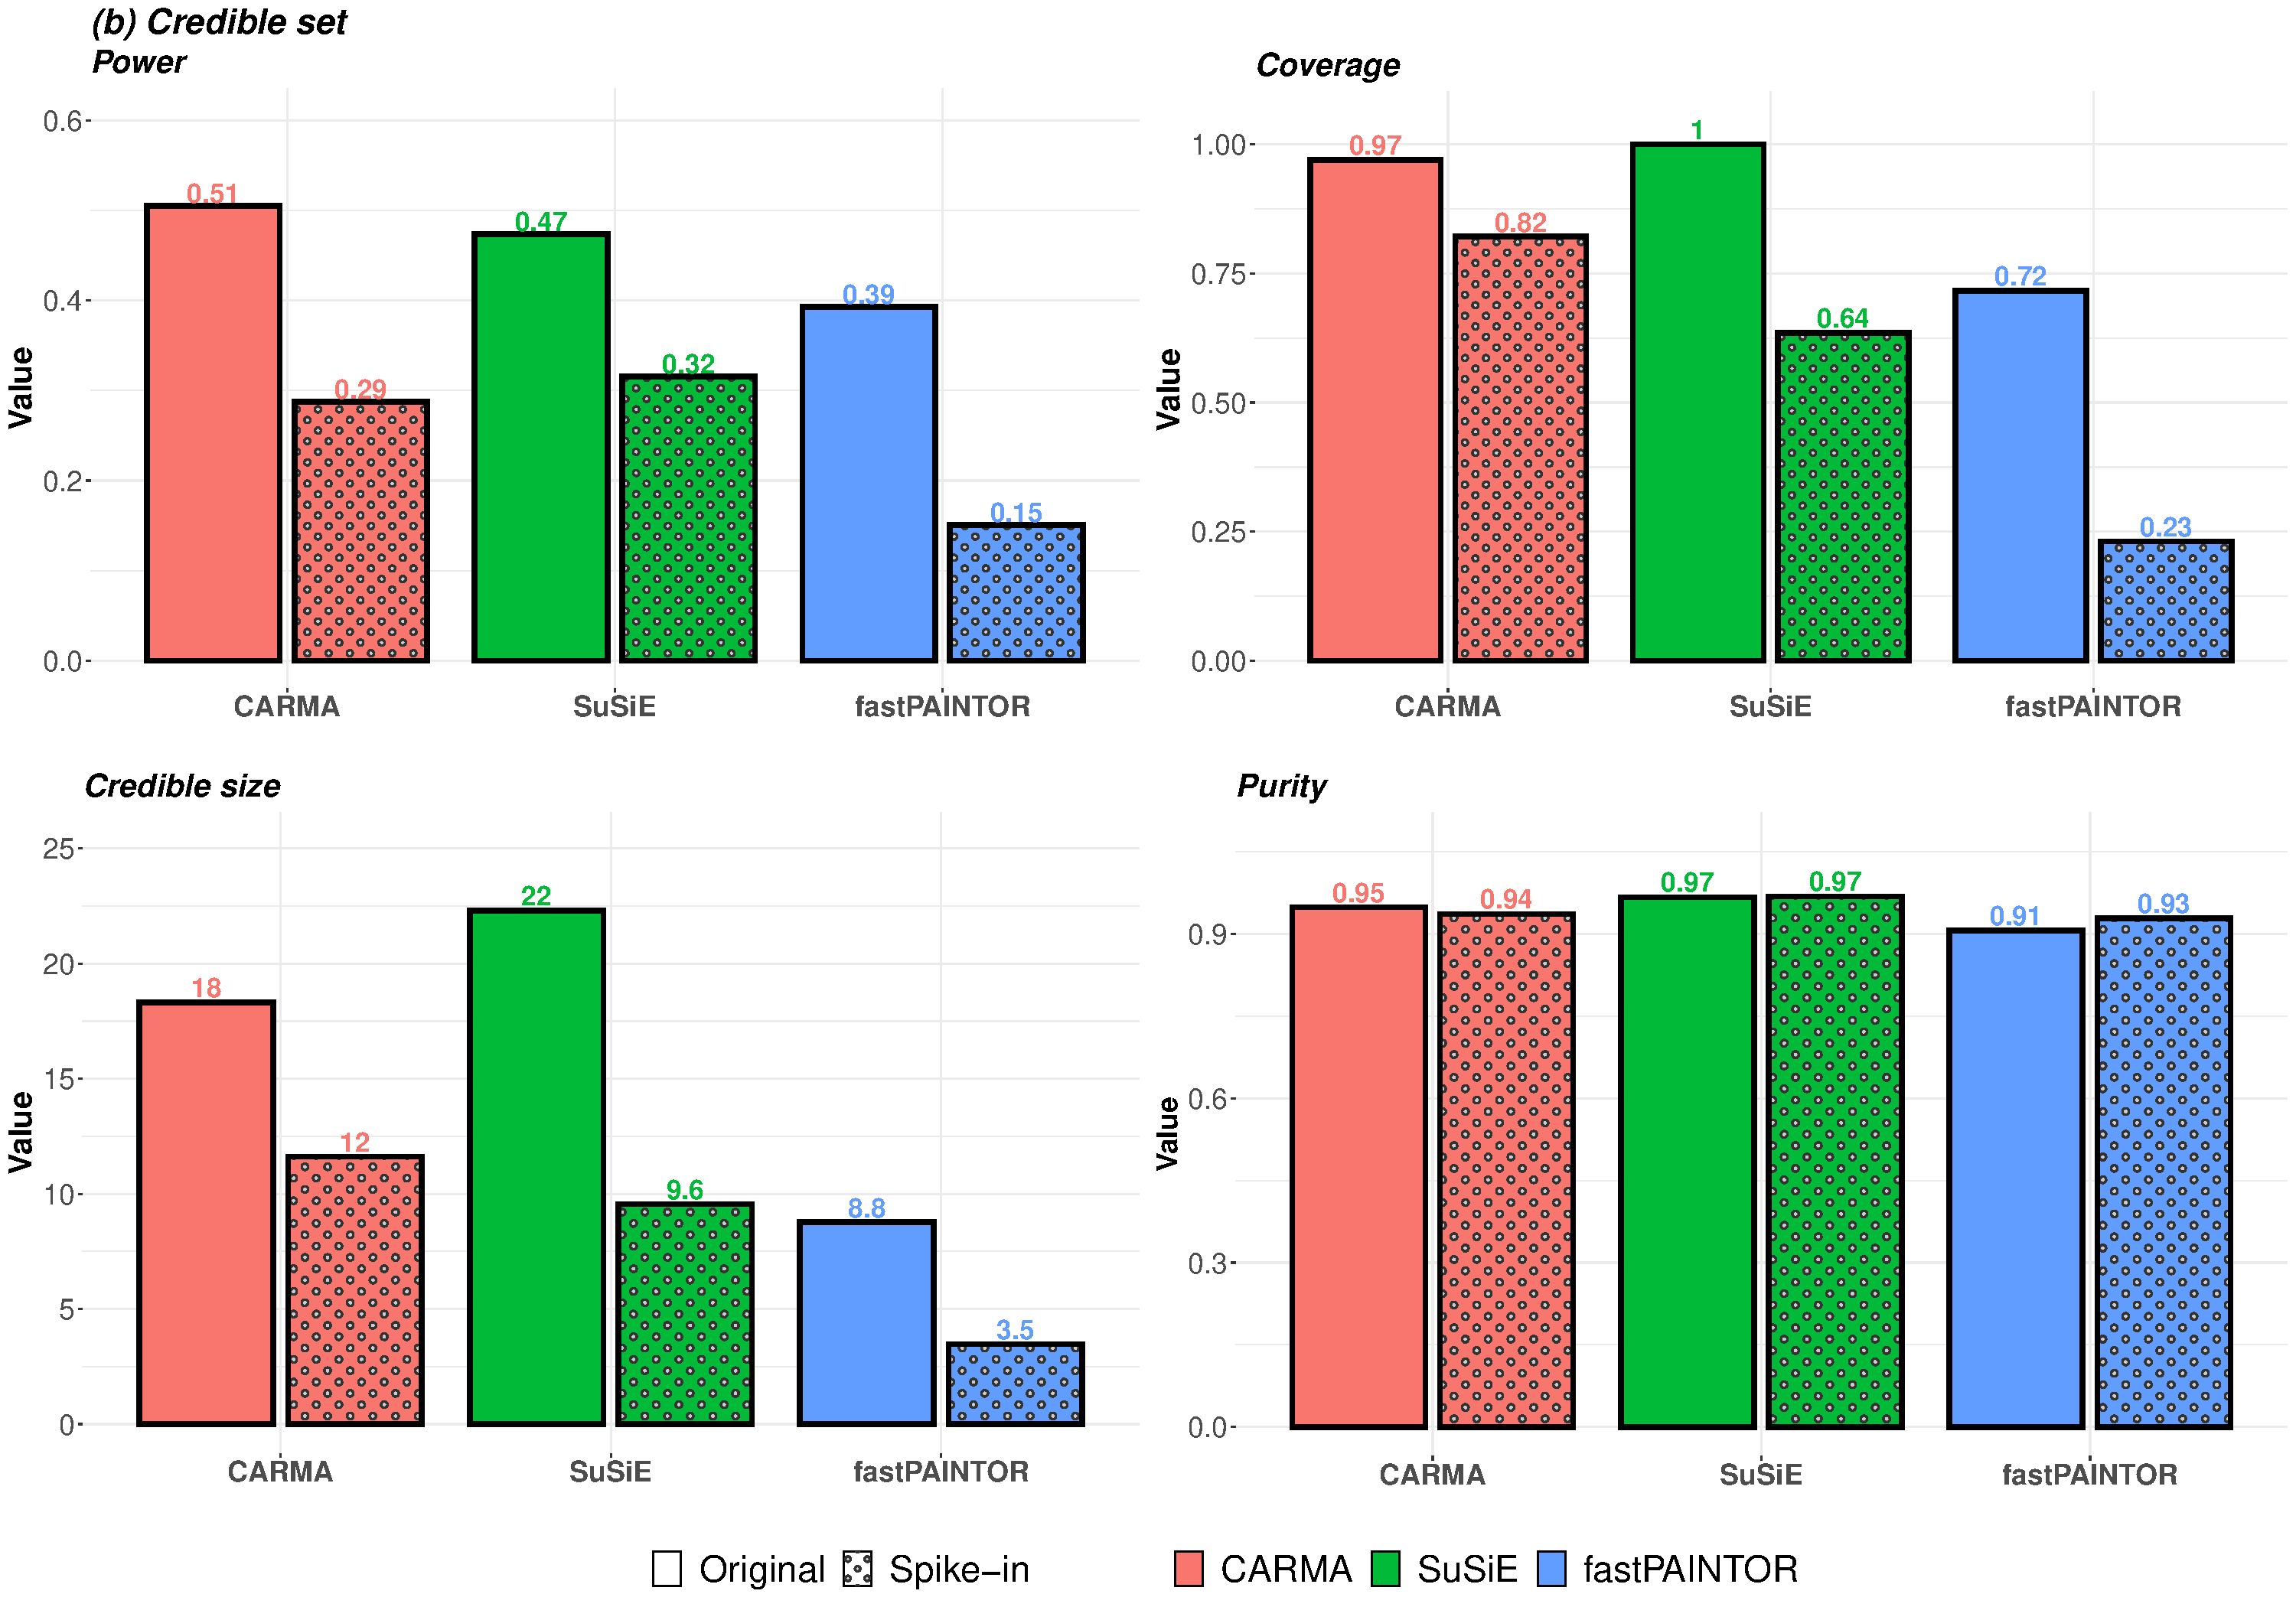
\includegraphics[width=2.5in]{./plots/normal_outlier_credible_set_|T|=3.pdf} 
 %  \caption{example caption}
   \label{fig:example}
   \end{figure}
   \end{column}%
\hfill%
\begin{column}{0.48\textwidth}
\begin{figure}[htbp] %  figure placement: here, top, bottom, or page
   \centering
   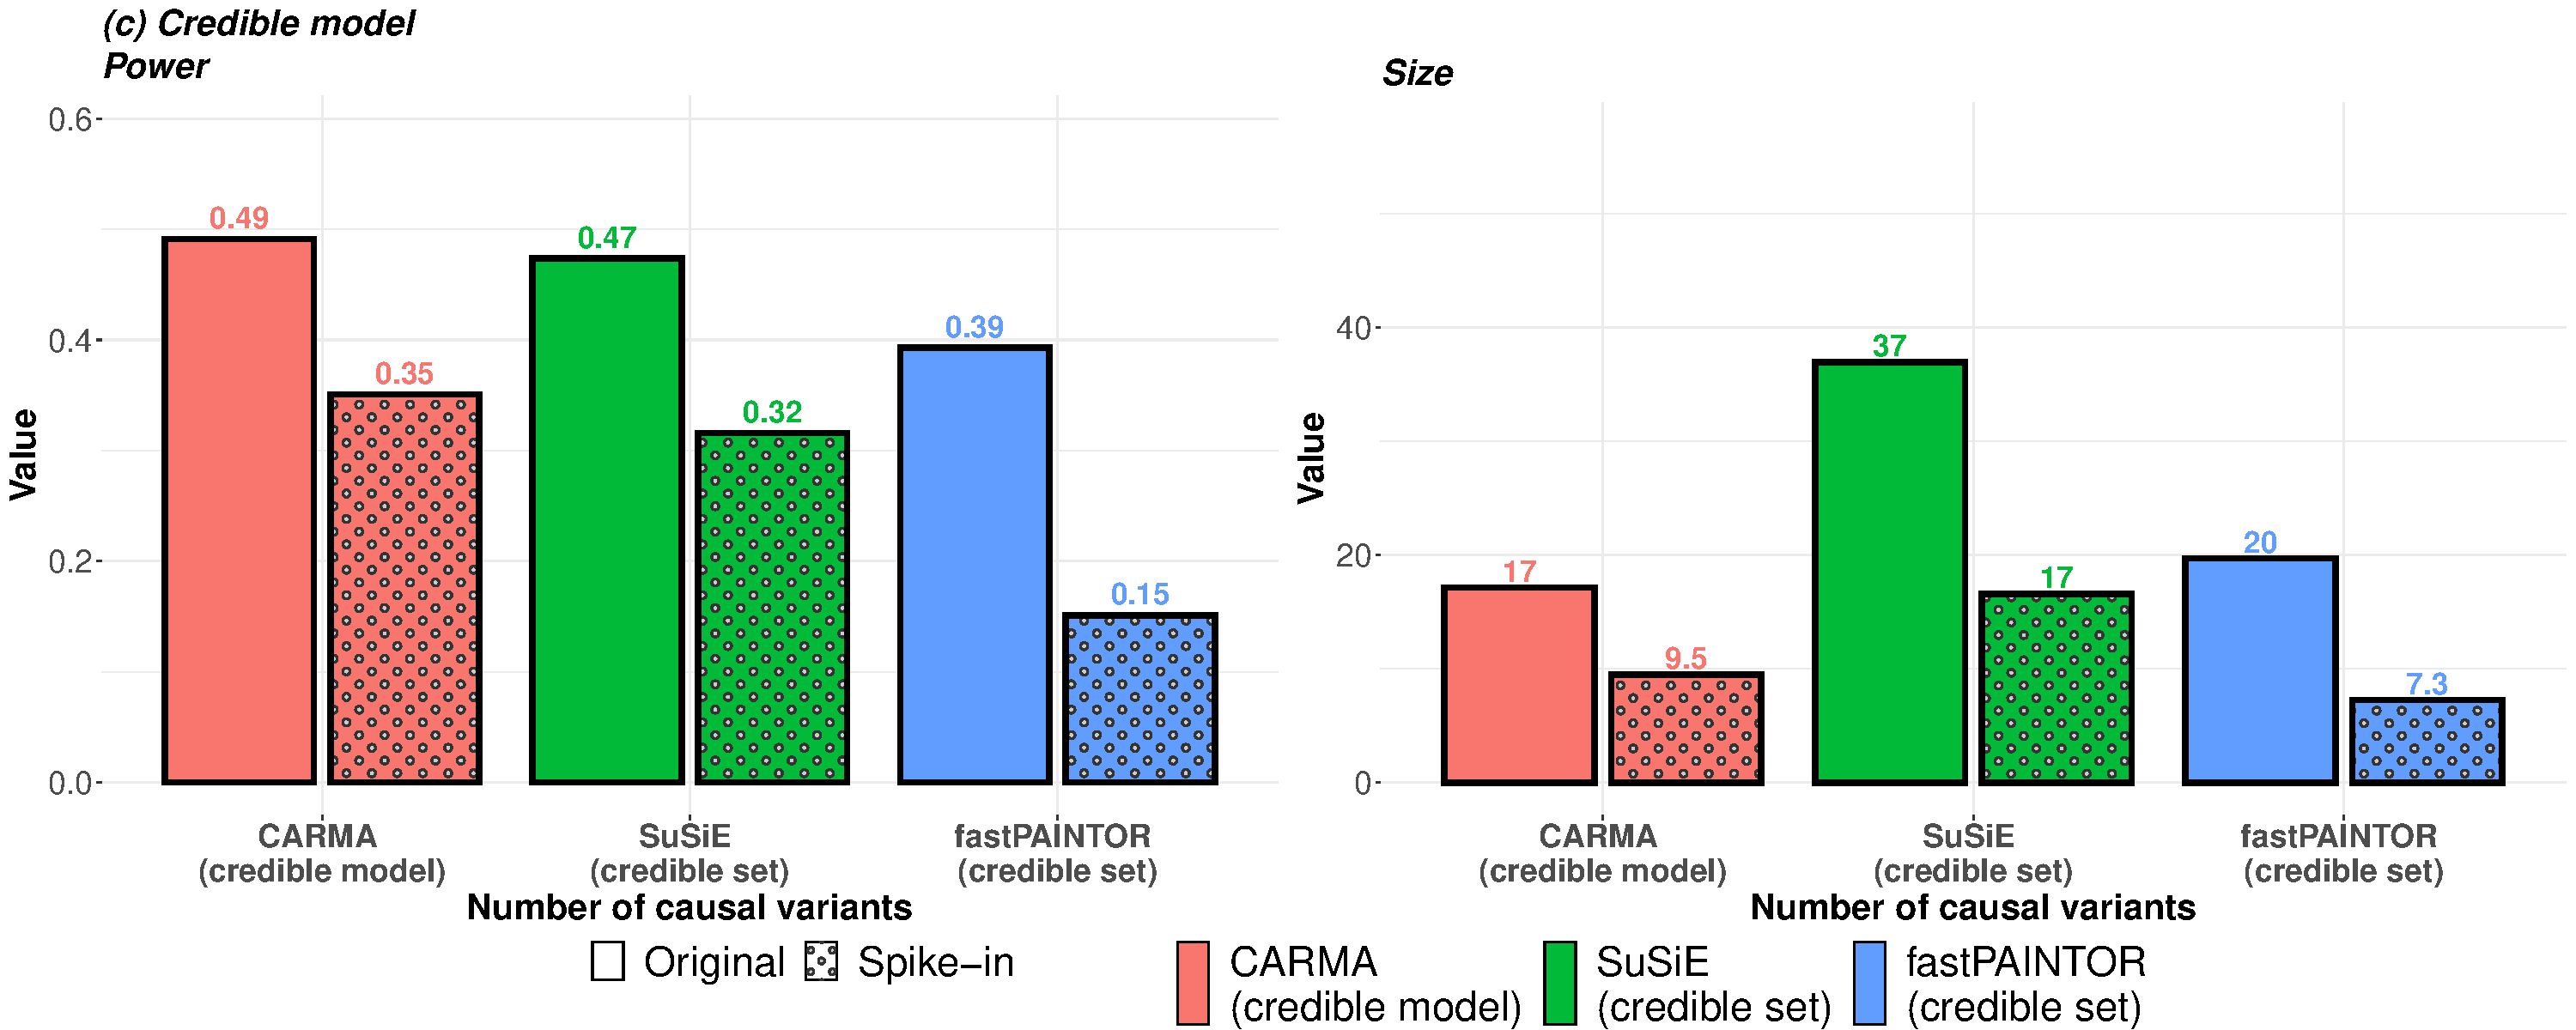
\includegraphics[width=2.5in]{./plots/normal_outlier_credible_model_|T|=3.pdf} 
  % \caption{example caption}
   \label{fig:example}
\end{figure}
\end{column}%
\end{columns}
}
%%%%%%%%%%%%%%%%%%%%%%%%%%%%%%%%%%%%%%%%%%%%%%%%%%%%%%%%%%%%%%%%%%%%%%%%%%%%%%%%%%%%%%
\frame{
\frametitle{Simulation results (with outlier)}
\begin{figure}[htbp] %  figure placement: here, top, bottom, or page
   \centering
   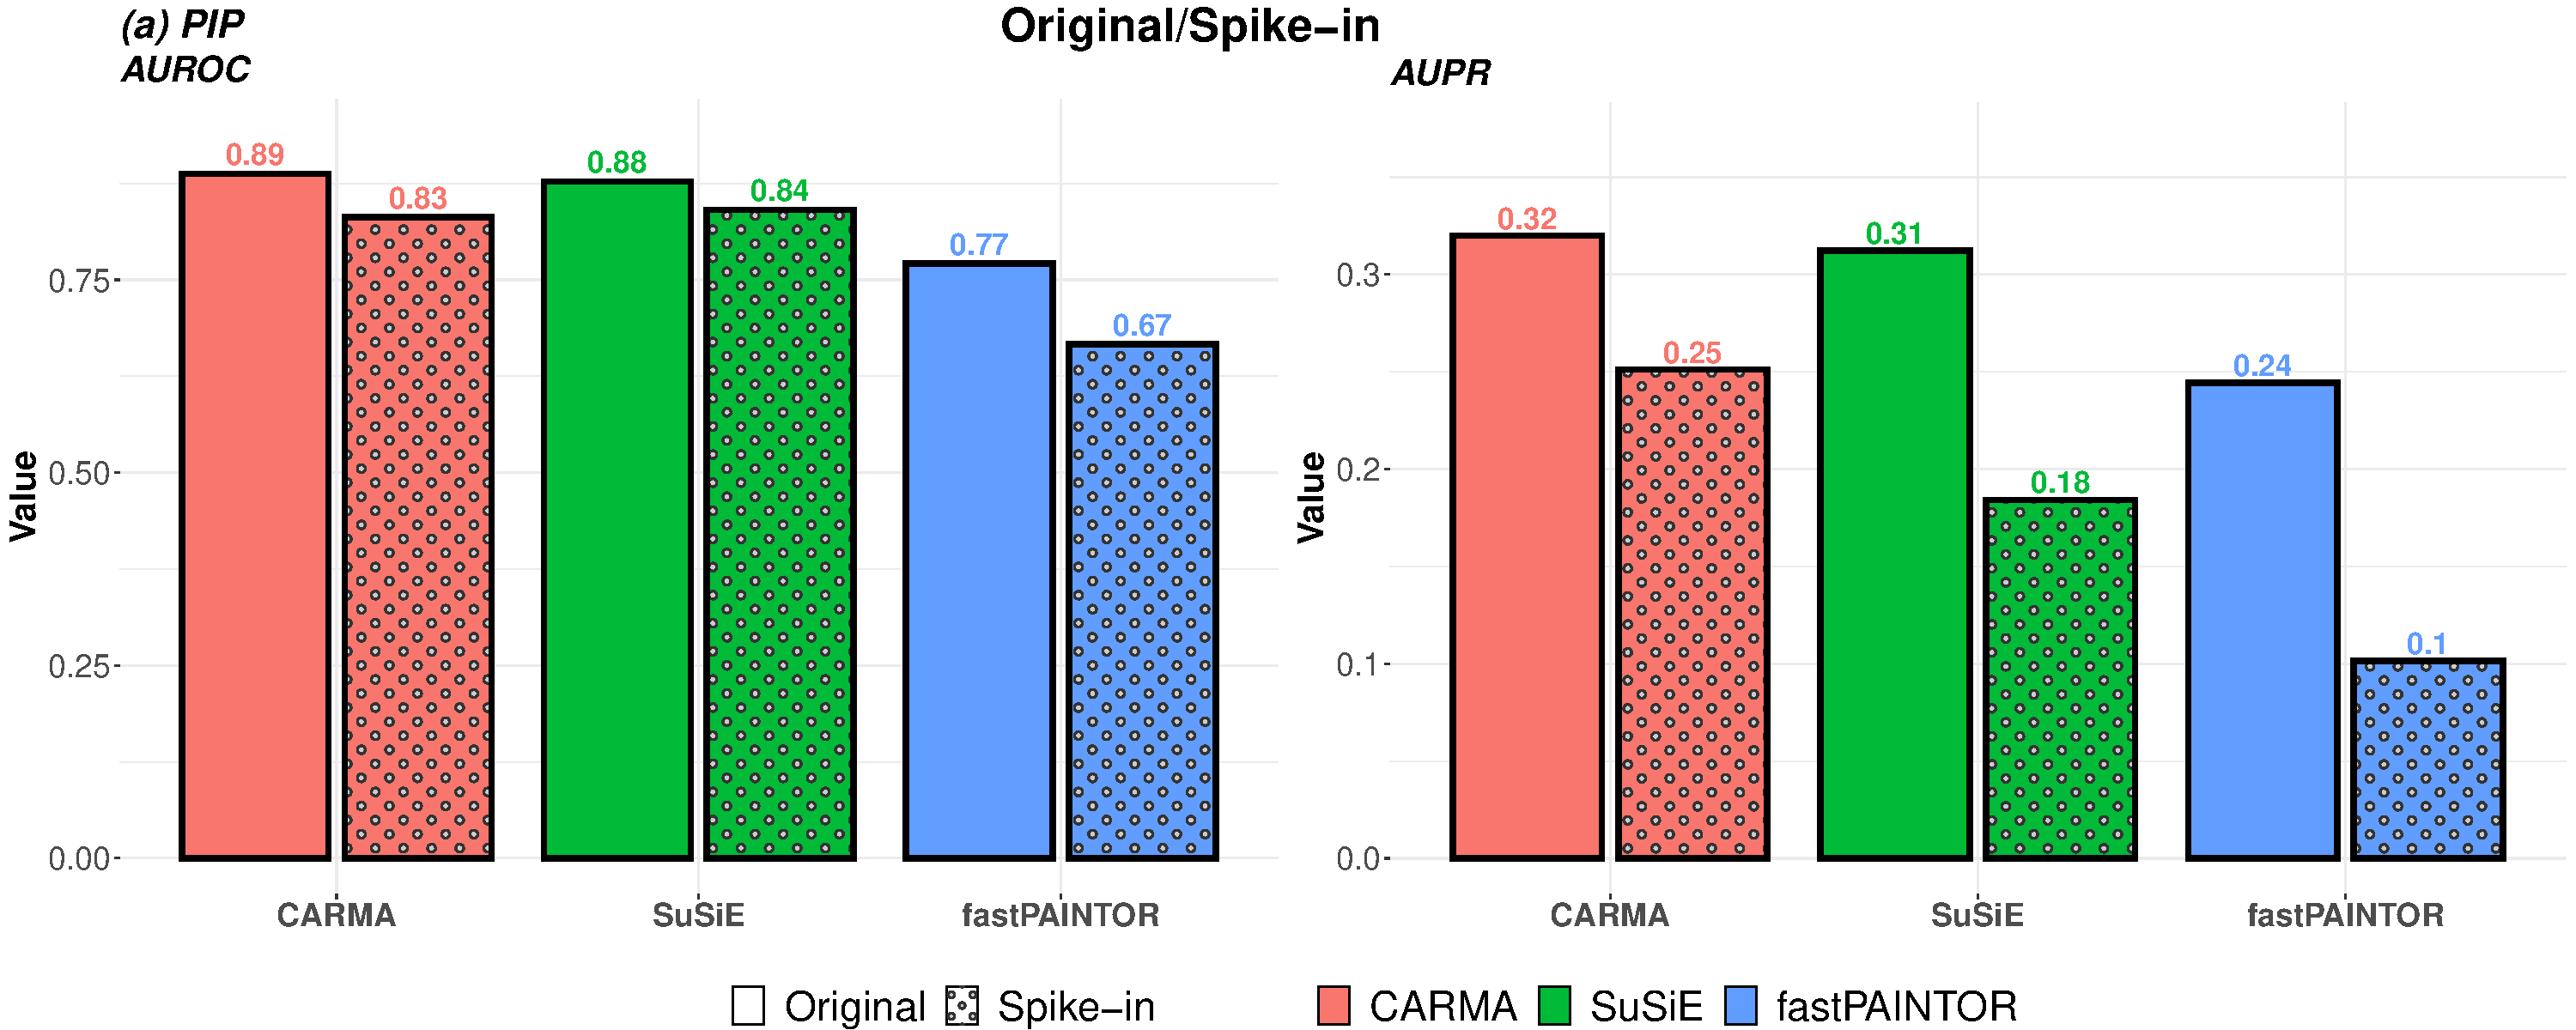
\includegraphics[width=4.5in]{./plots/normal_outlier_AUPR_AUROC_|T|=3.pdf} 
%      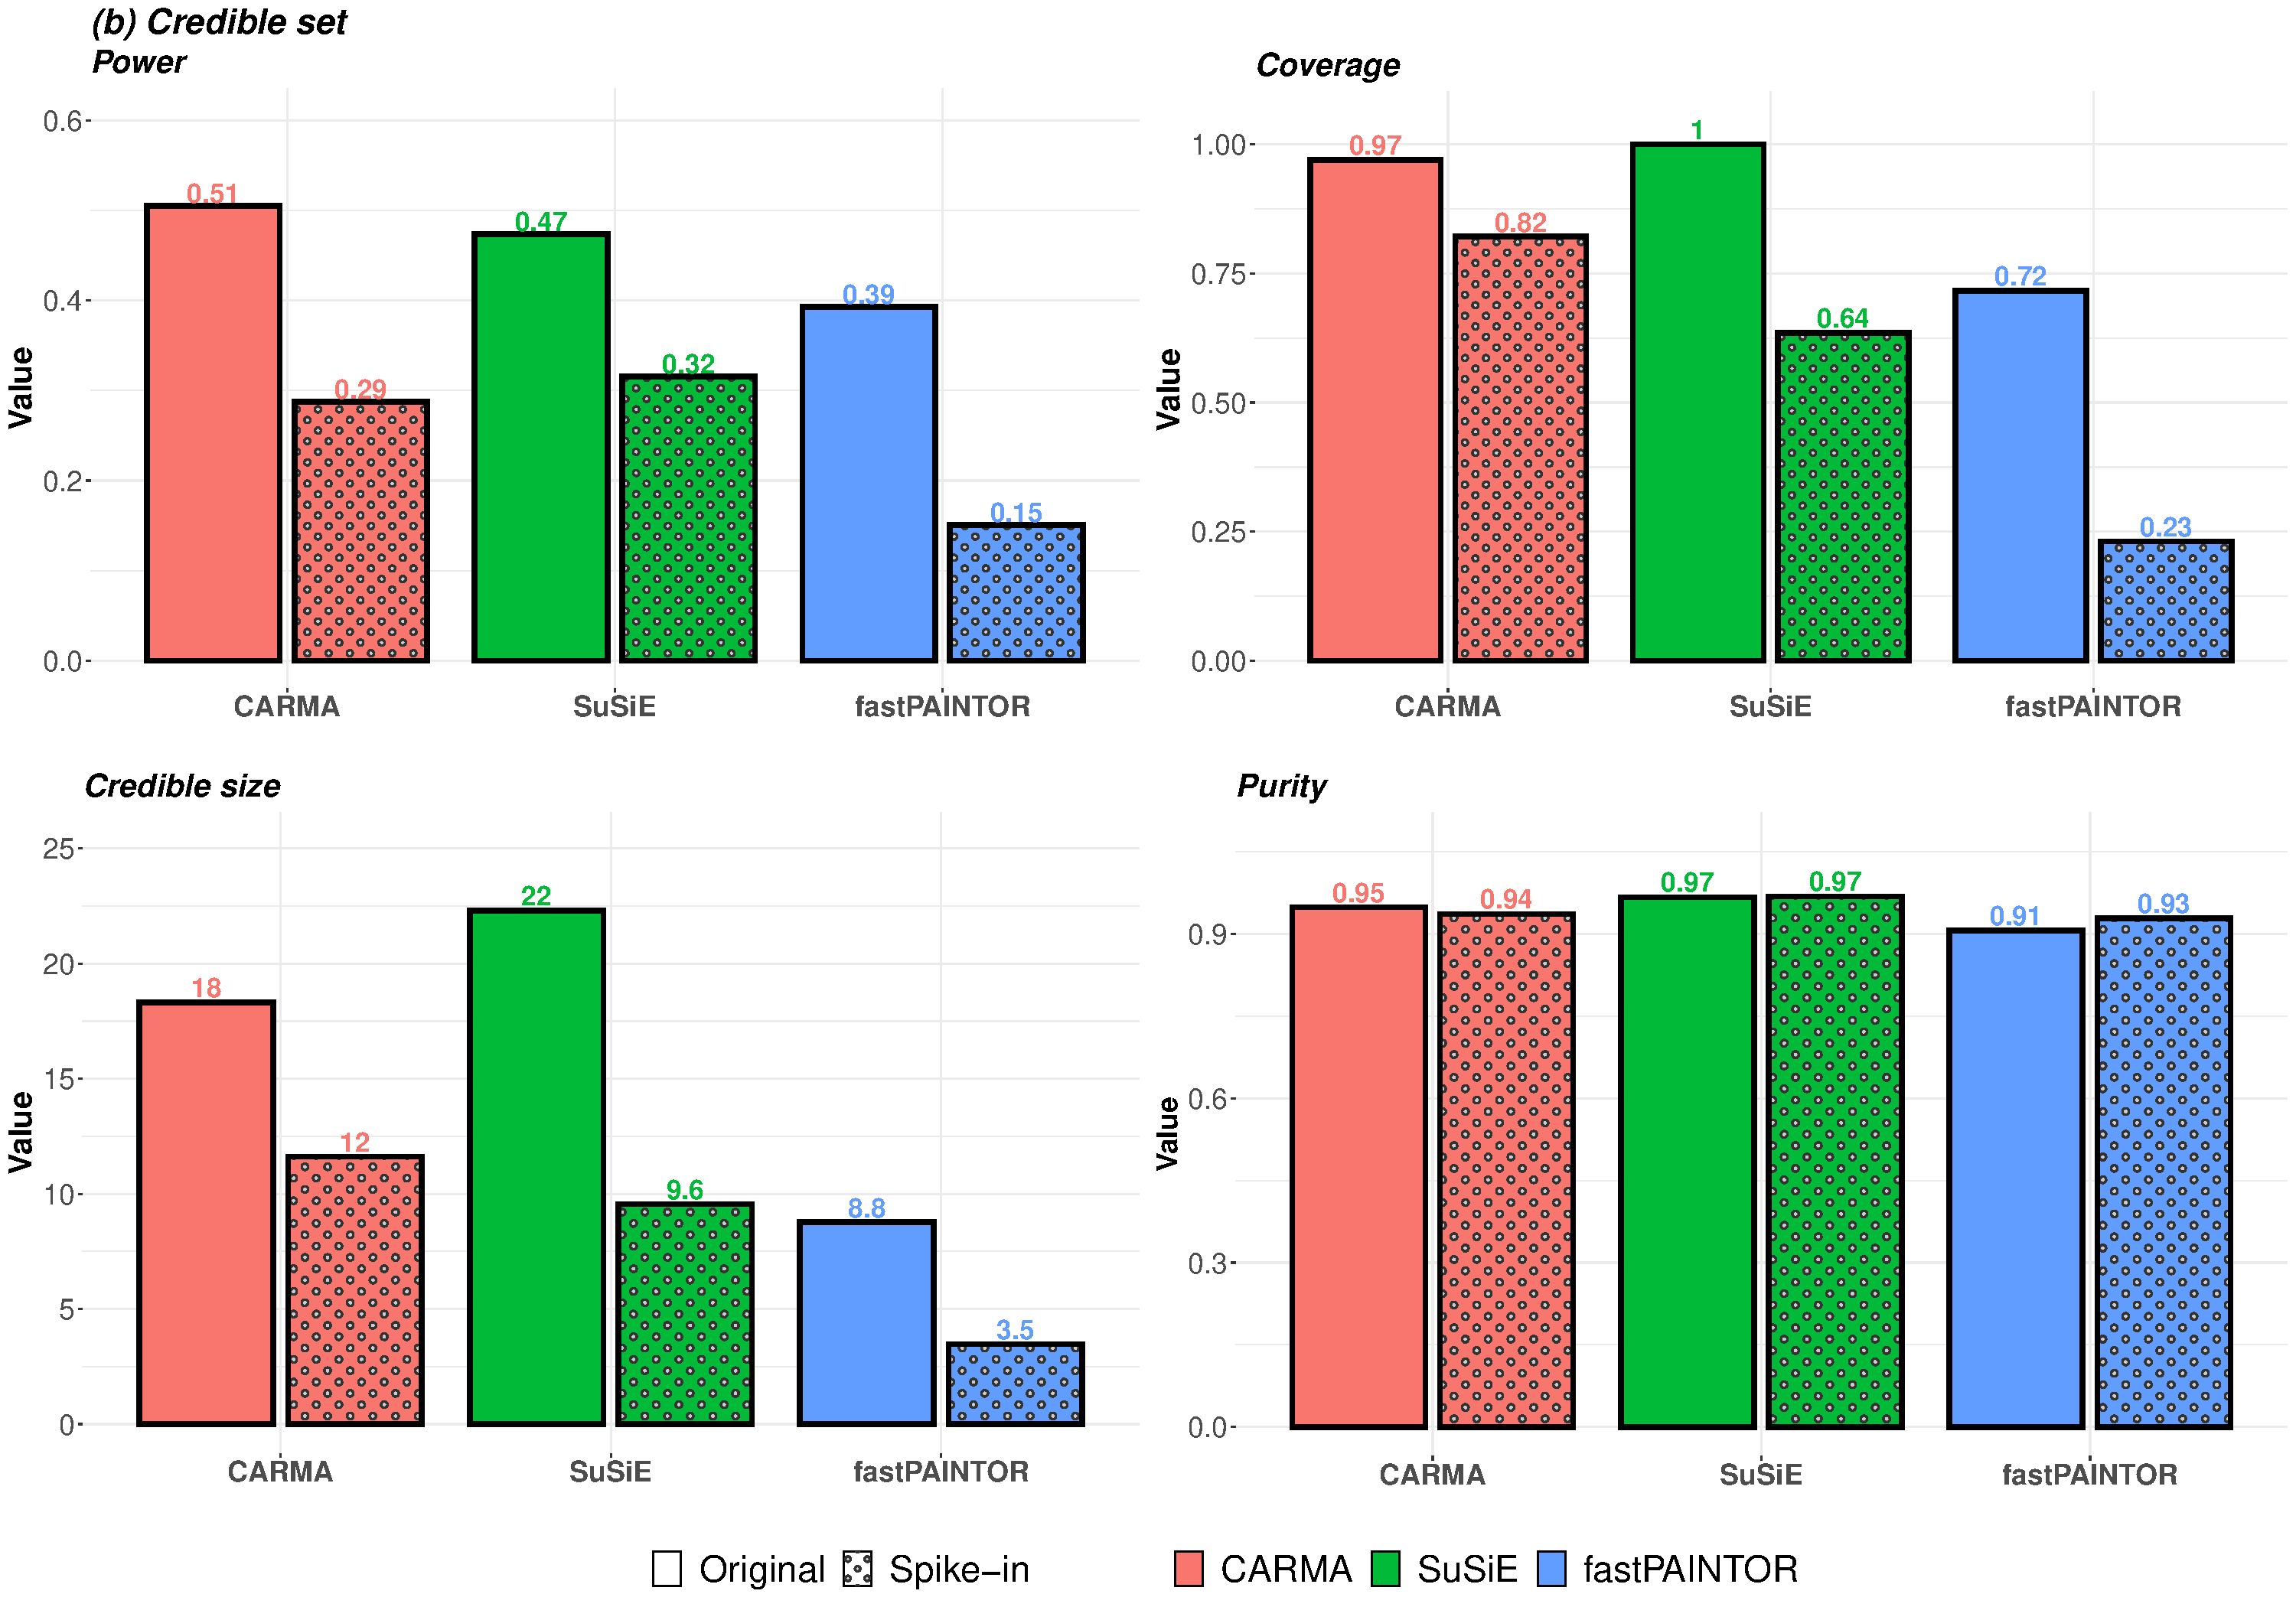
\includegraphics[width=2.5in]{./plots/normal_outlier_credible_set_|T|=3.pdf} 
 %  \caption{example caption}
   \label{fig:example}
   \end{figure}
}
%%%%%%%%%%%%%%%%%%%%%%%%%%%%%%%%%%%%%%%%%%%%%%%%%%%%%%%%%%%%%%%%%%%%%%%%%%%%%%%%%%%%%%
%%%%%%%%%%%%%%%%%%%%%%%%%%%%%%%%%%%%%%%%%%%%%%%%%%%%%%%%%%%%%%%%%%%%%%%%%%%%%%%%%%%%%%
\frame{
\frametitle{Outlier algorithm}
 \begin{algorithm}[H]
 \footnotesize
 At any step of the Shotgun algorithm, suppose that the current model is $\gamma_S$. \\
 Input: The index set  $S=\lrc{s_1,\ldots,s_{|S|}}$ for the current model $\gamma_S$, the threshold on the Bayes factor $\delta$, and the threshold on the correlation $\rho_{\text{outlier}}$. \\
\medskip

 \For{$s=1,\ldots,|S|$}{
  \begin{itemize}
  \item[-] Given $s_s\in S$, identify the group of  highly correlated SNPs indicated by the index  set $D=\lrc{i;~ \text{cor}\lrp{Z_{s_s},Z_i}\ge r_{\text{outlier}} \text{ for } \forall i \in \lrc{1,\ldots,p}}$.
  \item[-] Define $\tilde{\boldsymbol Z}=\lrc{Z_1,\ldots,Z_{|D|}}'$ as the summary statistics vector of the set $D$  .\\
   \Repeat{$\hat{B}_d\ge\delta$, for $\forall d\in\lrc{1,\ldots,|D|}$}{
      \For{$d=1,\ldots,|D|$}{
   \begin{itemize}
   \item[-] Define the hypothesis test for $Z_d$, such that
   \[
   \begin{array}{lcl}
H_0: Z_d\sim N(\beta,1);&& \text{ $Z_d$ is not an outlier}\\
 H_1: Z_d\sim N(\beta,c),~c\neq1;&& \text{ $Z_d$ is an outlier}. 
\end{array}
\]
\item[-] Compute the corresponding Bayes factor $\hat{B}_{d}$ conditional on $\tilde{\boldsymbol Z}_{D_{-d}}$ and $\boldsymbol\Sigma_{D_{-d}}$. 
   \end{itemize}=
   }
   
   \uIf{${ \exists} d\in \lrc{1,\ldots,|D|}, \hat{B}_{d}<\delta$}{
\begin{itemize}
  \item[-] Drop $Z_d$, where $\hat{B}_{d}=\text{min}\lrp{\lrc{\hat{B}_{1},\ldots,\hat{B}_{|D|}}}$, from the fine-mapping computation. 
    \item[-] Drop $Z_d$ from $\tilde{\boldsymbol Z}$, i.e., $\tilde{\boldsymbol Z}=\lrc{Z_1,\ldots,Z_{d-1},Z_{d+1},\ldots,Z_{|D|}}'$. 
  \item[-] Drop $d$th index from the index set $D$. 
    \end{itemize}
  
  }
   }
  \end{itemize}
 }
\setcounter{algocf}{1}
  \caption{The outlier detection procedure implemented in Shotgun algorithm.}
        \label{al::outlier} 
\end{algorithm}~\\
}
%%%%%%%%%%%%%%%%%%%%%%%%%%%%%%%%%%%%%%%%%%%%%%%%%%%%%%%%%%%%%%%%%%%%%%%%%%%%%%%%%%%%%%

\end{document}

%%%%%%%%%%%%%%%%%%%%%%%%%%%%%%%%%%%%%%%%%%%%%%%%%%%%%%%%%%%%%%%%%%%%%%%%%%%%%%%%%%%%%%
%%%%%%%%%%%%%%%%%%%%%%%%%%%%%%%%%%%%%%%%%%%%%%%%%%%%%%%%%%%%%%%%%%%%%%%%%%%%%%%%%%%%%%
\frame[t]{
\frametitle{Data structure for the fine-mapping methods}
\fontsize{7pt}{7pt}
\begin{block}{Basic setting of fine-mapping: a linear regression model}
\begin{itemize}
\item Given $n$ subjects and $p$ variants in a locus,  we assume 
\begin{equation*}
\boldsymbol Y=\boldsymbol X\boldsymbol\beta+\boldsymbol\epsilon, \text{ $\boldsymbol\epsilon\sim \text{MVN}(0,\sigma^2_y I_n)$}.
\end{equation*}
\item   $\boldsymbol Y$ is a quantitative phenotype vector standardized and adjusted by the common covariates.
\item   $\boldsymbol\epsilon$ is the Gaussian error vector. 
\item $\boldsymbol X$ is a $n\times p$ standardized genotype matrix.
\item $\boldsymbol\beta$ is a $p$-dimensional vector of effect size of SNPs. 
\item \textbf{Caveat}: The genotype matrix $X$ is usually too large to be shared across studies or researches. 
\end{itemize}
\end{block}
Due to logistic reason and the availability of meta-analysis, people use summary statistics and LD matrix instead. 

\begin{block}{Re-state the goal of fine-mapping}
Prioritizing the causality of genetic variants by the estimated posterior inclusion probability, 
\[
\Prob{\text{$i$th SNP is causal}|\boldsymbol Z, \Sigma},\]
based on the Z-scores $\boldsymbol Z$ and LD matrix $\Sigma$ instead of the phenotypes $Y$ and  genotypes $X$.
\end{block}
}
\begin{block}{Data for a given locus with $p$ variants and $n$ subjects}
\begin{itemize}
\item  We assume that we have genotype ($\boldsymbol{X}$) and phenotype ($\boldsymbol{y}$) data for $n$ subjects. 
\item We assume a standard linear model $\boldsymbol{y}=\boldsymbol{X}\boldsymbol\beta+\boldsymbol\epsilon, \text{ $\boldsymbol\epsilon\sim \text{MVN}(0,\sigma^2_y I_n)$}$
 \item  $\boldsymbol{y}$ is a $n\times 1$ vector of quantitative phenotype values adjusted by the common covariates 
 \item $\boldsymbol{X}$ is a standardized $n\times p$ genotype matrix
 \item  $\boldsymbol\beta$ is a $p$-dimensional vector of effect sizes of variants, and $\boldsymbol\epsilon$ is a Gaussian noise vector.
\end{itemize}
\end{block}


\begin{block}{The marginal association test}
\begin{itemize}
\item In a given genomic region (Locus), there are $p$ variants and $n$ subjects. 
\item For each variant $i$, $i=1,\ldots,p$, we obtain the estimated marginal effect $\hat{\beta}_i(=\frac{\boldsymbol x_i'\boldsymbol y}{\boldsymbol x_i'\boldsymbol x_i})$ and standard error $\text{se}\lrp{\hat{\beta}_i}$. 
\item The Z-score is defined as $Z_i=\frac{\hat{\beta}_i}{\text{se}\lrp{\hat{\beta}_i}}$ of Wald test ($\hat{\beta}_i$), with $Z_i\sim N(0,1)$ under the null hypothesis $H_0:\beta_i=0$.
\item Let $\boldsymbol \lambda\propto \boldsymbol \beta$ (i.e., $\lambda_i\neq0$ if and only if $\beta_i\neq0$). The sampling distribution of $\boldsymbol Z$ can be written as:
 $$
 \boldsymbol Z| \boldsymbol\lambda,\sigma^2_y,\boldsymbol\Sigma \sim\text{MVN}(\boldsymbol\Sigma\boldsymbol\lambda,\sigma^2_y\boldsymbol\Sigma), 
$$
 where $\boldsymbol{\Sigma}=\frac{\boldsymbol{X'X}}{n}$ is the LD correlation matrix.
 \item We assume $\boldsymbol \lambda$ is a sparse vector, and want to identify non-zero entries of  $\boldsymbol \lambda$ associated with the causal variants. 
\end{itemize}
\end{block}

%%%%%%%%%%%%%%%%%%%%%%%%%%%%%%%%%%%%%
%%%%%%%%%%%%%%%%%%%%%%%%%%%%%%%%%%%%%

